\documentclass[master=cws, masteroption=vs,english]{kulemt}

% Vul de titel van jouw masterproef hieronder in tussen { en }.

\setup{title={Flip the virus:  Modelling targeted attacks using FlipIt with propagation delay},
%
% Vul hieronder namen in, steeds Voornaam Naam.
% Indien meerdere auteurs, assessoren, assistenten, scheidt hun namen
% met \and .
author={Sophie Marien},
promotor={Prof. dr. T. Holvoet},
assessor={Prof. dr. B. Jacobs \and Dr. ir. A. Dries},
assistant={Ir. Jonathan Merlevede, \and Ir. Kristof Coninx}}
% 
% De volgende \setup mag verwijderd worden als geen fiche gewenst is.
\setup{filingcard,
  translatedtitle={Flip the virus:  Modelling targeted attacks using FlipIt with propagation delay},
  udc=621.3,
  shortabstract={Recently, high profile targeted attacks such as the
attack on Belgacom (a major Belgian telcom), have demonstrated
that even the most secure companies can still be compromised,
and that moreover such attacks can go undetected for a while. These kind of attacks are called APT, advanced persistent threats, which are designed to penetrate secretly a computer network, collect sensitive data and stay hidden for many years. A company has every interest to mitigate the risks of an APT and the consequences that it can cause.  Because of the stealthiness fighting against these attacks requires methods that go beyond the standard tools against malware.
A group of researchers at the RSA, van Dijk et al., proposed the game FlipIt (The game of ``stealthy takeover'') to model stealthy takeovers. It is a 2-players game composed of
a single attacker, a single defender and a single shared resource.
The players will 
compete to get control over the shared resource. Every move of the players will involve a cost and
these moves happen in a stealthy way. The objective of the game for each player is to maximise the fraction of time of controlling the resource and minimise the total move cost.  \\
FlipIt does however not take into
account that a move may not be instantaneous, but has a certain
delay.  We adapt FlipIt such that we can use it to
model the game of defending a company network that is attacked
by a virus. The FlipIt formulas are adapted such as to take the
delay for virus propagation into account, which in our case will be a delay for the attacker. In this paper, we restrict ourselves to games where both the defender and the attacker play with a periodic strategy. The goal of this thesis is to find out if their are interesting Nash Equilibria for a game with a virus propagation delay and if we can learn some lessons out of it. }}
% Verwijder de "%" op de volgende lijn als je de kaft wil afdrukken
%\setup{coverpageonly}
% Verwijder de "%" op de volgende lijn als je enkel de eerste pagina's wil
% afdrukken en de rest bv. via Word aanmaken.
%\setup{frontpagesonly}

% Kies de fonts voor de gewone tekst, bv. Latin Modern
\setup{font=lm}

% Hier kun je dan nog andere pakketten laden of eigen definities voorzien
\usepackage{graphicx}
\usepackage{amsmath}
\usepackage{amssymb}
\usepackage{listings}
\usepackage{color}
\usepackage{soul}
\usepackage{tikz}
\usepackage{parskip}
\usepackage{todonotes}
\usepackage{url}
\usepackage{natbib} 
%\usepackage{pgf}
\usepackage{tikz}
\usepackage{hyperref}
\usepackage[font={small,it}]{caption}
\usepackage[english]{babel}
%\headstyles{kulemtman}


%\usepackage{float}
%\usepackage{caption}
%\usepackage[caption = false,subrefformat=parens,labelformat=parens]{subfig}
%\usepackage{todonotes}
%\usepackage{epstopdf}
%\usepackage{textcomp}
%\usepackage{gensymb}
%\usepackage[titlenumbered,algoruled, linesnumbered]{algorithm2e}
%\usepackage{algpseudocode}
%\usepackage{parskip}
%\usepackage{kulemtx}
%\headstyles{kulemtman}
%
%\DontPrintSemicolon



\usetikzlibrary{arrows,automata}
%\usepackage[latin1]{inputenc}
\definecolor{dkgreen}{rgb}{0,0.6,0}
\definecolor{gray}{rgb}{0.5,0.5,0.5}
\definecolor{mauve}{rgb}{0.58,0,0.82}

%\lstset{frame=tb,
%  language=Java,
%  aboveskip=3mm,
%  belowskip=3mm,
%  showstringspaces=false,
%  columns=flexible,
%  basicstyle={\small\ttfamily},
%  numbers=none,
%  numberstyle=\tiny\color{gray},
%  keywordstyle=\color{blue},
%  commentstyle=\color{green},
%  stringstyle=\color{black},
%  breaklines=true,
%  breakatwhitespace=true
%  tabsize=3
%}

%\newcommand{\todo}[1]{{\huge \textcolor{green}{#1}}\\}
%\newcommand{\com}[1]{\textcolor{red}{#1}\\}
%\newcommand{\viscomment}[1]{\textcolor{red}{#1}}
\newcommand{\flip}[1] {\textcolor{black}{#1}}

% Tenslotte wordt hyperref gebruikt voor pdf bestanden.
% Dit mag verwijderd worden voor de af te drukken versie.
%\usepackage[pdfusetitle,colorlinks,plainpages=false]{hyperref}

%%%%%%%
% Om wat tekst te genereren wordt hier het lipsum pakket gebruikt.
% Bij een echte masterproef heb je dit natuurlijk nooit nodig!
\IfFileExists{lipsum.sty}%
 {\usepackage{lipsum}\setlipsumdefault{11-13}}%
 {\newcommand{\lipsum}[1][11-13]{\par Hier komt wat tekst: lipsum ##1.\par}}
%%%%%%%


%\includeonly{chap-n}
\begin{document}

\begin{preface}
Thank you !

%Ten slotte gaat mijn grootste dank uit naar mijn ouders. Zij leverden
%niet alleen een cruciale bijdrage aan het welslagen van deze
%meesterproef, maar zijn een belangrijke hulp voor mijn academische
%studies in het geheel. Zonder hen zou niets wat ik tot nu toe heb
%bereikt, mogelijk geweest zijn
% Many people have helped in the realization of this thesis. 
%  I would like to thank everybody who kept me busy the last year and made it possible for me to finish my thesis.\\
%  
%  First I would like to thank my promoter and my assistants for their excellent support during the writing of this paper. They helped me figure out what to do and put a lot of time and effort in me.\\
%  
%   
%   I would also like to thank my boyfriend who supported me during the writing of this thesis and helped me to write a beautiful text.  \\
%   
%   Last but not least all the people that read my thesis for faults: .. \\
%   A few other people earn a special mention: Revue-blokt for keeping me focused on my thesis, DistriNet labo for letting me in and study in a quit place, Antonio for distracting me and telling me stories about his travels.
%   A special memorial to John Nash, a mathematician with a fundamental contribution to Game Theory, that died in a car accident during the writing of this thesis. His Nash Equilibrium is used in this thesis.. \\
 
\end{preface}

\tableofcontents*
\listoftodos
\begin{abstract}

%  The \texttt{abstract} environment contains a more extensive overview of  the work. But it should be limited to one page.
  
Recently, high profile targeted attacks such as the
attack on Belgacom (a major Belgian telcom), have demonstrated
that even the most secure companies can still be compromised,
and that moreover that such attacks can go undetected for a while. This kind of attack is called APT, Advanced Persistent Threats, and designed to secretly penetrate a computer network, collect sensitive data and stay hidden for many years. Companies have every interest to mitigate the risks of an APT and the consequences that it can cause.  Because of stealthiness, fighting against this kind of attack requires methods that go beyond the standard tools against malware.\\
A group of researchers at the RSA, van Dijk et al., proposed the game FlipIt (The game of ``stealthy takeover'') to model stealthy takeovers. It is a 2-players game composed of
a single attacker, a single defender and a single shared resource.
The players will 
compete to get control over the shared resource. Every move of the players will involve a cost and
these moves happen in a stealthy way. The objective of the game for each player is to maximise the fraction of time being in control of the resource and minimise the total move cost.  \\
FlipIt does however not take into
account that a move may not be instantaneous, but may have a certain
delay.  We adapt FlipIt such that we can use it to
model the game of defending a company network that is attacked
by a virus. The FlipIt formulas are adapted such as to take the
delay for virus propagation into account, which in our case will be a delay for the attacker. In this paper, we restrict ourselves to games where both the defender and the attacker play with a periodic strategy. The goal of this paper is to find out if modelling such situations with FlipIt with propagation delay allows us to draw interesting lessons about security measures against APT's.  
\todo{Results toevoegen} \\

\textbf{Keywords}: Game theory, Advanced persistent threats, cyber security, FlipIt, stealthy takeovers, propagation methods.

\end{abstract}

\begin{abstract*}
Nederlandse abstract
---TODO dit stuk moet nog geschreven worden --- \\

Security is een niet te missen aspectgeworden in de technologie. Door de vooruitgang en betere technologie"en worden security aanvallen veel geavanceerder en moeilijker te bestrijden. Onlangs zijn er gerichte security aanvallen geweest op grote bedrijven, zoals de aanval op Belgacom (een grote Belgische telcom). Deze aanvallen hebben aangetoond dat zelfs de meest veilige
bedrijven nog steeds gecompromitteerd kunnen worden, en dat bovendien dergelijke aanvallen onopgemerkt kunnen blijven voor een bepaalde tijd. \\

Vele bedrijven hebben grote databases die belangrijke informatie bevatten zoals bijvoorbeeld vertrouwelijke informatie over klanten. Het is belangrijk dat deze informatie binnen het bedrijf blijft. Computer en Network security zorgt ervoor dat bedrijven hun informatie kunnen beschermen tegen bedrijgingen. \\
Een van deze bedrijgingen die interessant is voor deze paper is een Advanced Persistent Threat (APT). Een APT is een continue en gerichte cyber aanval die ontworpen is om systemen en netwerken heimelijk binnen te dringen en dan voor een lange tijd onopgemerkt te blijven. Een manier om deze heimelijke aanvallen te analyseren is door het te modelleren via speltheorie. Speltheorie krijgt meer en meer belangstelling in het veld van security om cyber security problemen te modelleren. Deze problemen worden meestal gemodelleerd als een spel met twee spelers, een aanvaller en een verdediger. Er zijn ook probelemen die gemodelleerd kunnen worden als spelen met meerdere spelers, maar in de paper wordt gefocust op een spel met twee spelers. \\

In deze paper gaan we verder op een security spel ge"introduceerd door van Dijck et al, ``FlipIt'' \citep{FlipIt}.
Flipit is een speltheoretisch framework om computer scenarios te modelleren die een sthealty aspect hebben. Het is een 2-spelers spel bestaande uit een aanvaller, een verdediger en een gedeelde bron.  De spelers proberen om controle te krijgen over de gedeelde bron en ze
doen dit op een heimelijke manier. Met FlipIt wordt echter geen rekening mee gehouden dat een aanval niet onmiddellijk is, maar dat dit kan gebeuren met een zekere vertraging. In dit artikel passen we het model van FlipIt zodanig aan dat we het kunnen gebruiken voor heimelijke aanvallen die onderheven zijn aan een vertraging.
Resultaat : \\

Flipit is een spel ge"introduceerd door Van Dijk et al. Om te begrijpen hoe we het FlipIt spel kunnen aanpassen om virus propagatie in acht te nemen, is het belangrijk om vertrouwd te raken met de concepten van het basische Flipit spel en de notaties. Daarom beginnen we eerst met een uitleg hoe het basische FlipIt spel werkt en de belangrijkste formules die we in de paper gebruiken. \\

Flipit is een spel met twee spelers met een gedeelde bron die de spelers zo lang mogelijk willen beheren. De gedeelde bron kan een wachtwoord, een netwerk of een geheime sleutel zijn afhankelijk van welke situatie gemodelleerd wordt. In de rest van de paper noemen we de twee spelers de aanvaller, aangegeven met onderschrift  \textit{A} en de verdediger, aangegeven met onderschrift \textit{D}.

Het spel begint op tijdstip $ t = 0 $ en blijft voor onbepaalde tijd doorgaan ($ t \rightarrow \infty $). De tijd van het spel wordt aangenomen als continu. Om controle over de bron te krijgen kunnen de spelers $i$, met $ i \in \{A, D \} $ de bron flippen. Elke flip impliceert een zekere kost $ k_{i} $ en deze kosten kunnen vari"eren voor elke speler. Beide spelers proberen om hun kosten te minimaliseren. Door een kost in te voeren, voorkomt men dat de spelers te vaak bewegen. \\

De unieke eigenschap van Flipit is dat elke flip gebeurt op een heimelijke manier. Dit betekent dat de speler geen weet heeft over wie de controle heeft over de bron. Zo zal de verdediger niet kunnen achterhalen of de bron al is gefipt door de aanvaller tot hij de bron zelf flipt. Het doel van elke speler is om zo lang mogelijk de controle te behouden over de bron en tegelijkertijd de kost van de bewegingen te minimaliseren. Een beweging kan ook leiden tot een ``verloren bewegin'', genoemd een flop. Het kan gebeuren dat de bron reeds onder controle is van de speler. Als de speler flipt wanneer hij of zij al de controle  heeft over de bron, dan verspilt de speler een zet omdat het niet leidt tot een verandering van controle en dus een kost verspilt wordt. \\


\begin{figure}[hbtp]
\center
\includegraphics[scale=0.5]{../../doc/template/Images/DefFlipit}
\caption{Een afbeelding van een Flipit spel met discrete tijdsintervallen waarbij beide spelers periodiek spelen. Elke beweging of flip wordt aangegeven met een blauwe ( donkergrijs) of oranje (lichtgrijze) cirkel. De aanvaller is vertegenwoordigd in het oranje en speelt met een periode van $ \delta_{A} = 4 $. De verdediger is vertegenwoordigd in het blauw en speelt met een periode van $ \delta_{D} = 3 $. De blauwe en oranje rechthoeken geven de hoeveelheid tijd die de betreffende speler in de controle is van de bron.}
\label{fig: FLipItDefault}
\end{figure}



De toestand van de bron wordt aangeduid als een tijdsafhankelijke variabele $ C = C_{i}(t) $.
$ C_{D}(t) $ 1 is als het spel onder controle is van de verdediger en 0 als het spel onder controle is van de aanvaller. Omgekeerd, zal $ C_{A}(t) $ 1 zijn als het spel onder controle is van de aanvaller en 0 als onder controle van de verdediger. Dus, $ C_{A}(t) = 1 - C_{D}(t) $.
Het spel begint met de verdediger in controle: $ C_{D}(0) = 1 $. \\


De spelers krijgen een benefit gelijk aan de hoeveelheid tijd dat ze in het bezit zijn van de bron min de kosten voor het maken van de bewegingen. De kosten van een speler \textit{i} worden aangegeven met $ k_{i} $.
De totale winst van de speler \textit{i} is gelijk aan de totale hoeveelheid tijd waarbij een speler \textit{i} in controle is can de bron vanaf het begin van het spel tot de huidige tijd \textit{t}. Dit wordt als volgt uitgedrukt:
\begin{equation}
G_{i}(t) = \int_0^t \! C_{i}(x) dx.
\end{equation}
De totale winst van de verdediger opgeteld bij de totale winst van de aanvaller telt op tot \textit{t}:
\begin{equation} 
G_{D}(t) + G_{A}(t) = t
\end{equation}
De gemiddelde winst van speler \textit{i} wordt gedefinieerd als volgt:
\begin{equation}
\gamma_{i}(t) = G_{i}(t) / t.
\end{equation}
En daarmee voor alle $ t> 0 $:
\begin{equation} 
\gamma_{D}(t) + \gamma_{A}(t) = 1
\end{equation}
$ \alpha_{i} $ definieert het gemiddeld aantal flippen door speler \textit{i} tot tijd \textit{t}.
Laat $ \beta_{i}(t) $ is de gemiddelde benefit van een speler \textit{i} tot aan tijd \textit{t}:
\begin{equation}
\beta_{i}(t) = \gamma_{i}(t) - k_{i} \alpha_{i}.
\end{equation}
Dit is gelijk aan de fractie van de tijd waarbij de bron in handen is van speler \textit{i}, minus de kosten van het maken van de bewegingen. ~ 
Gedurende het spel wordt de asymptotische benefit ratio gedefinieerd als lim inf van de gemiddelde benefit omdat de tijd t toeneemt tot oneindig en de gemiddelde benefit heeft niet altijd een limiet.
\begin{equation}
\beta_{i} (t) = \lim_{t \to \infty } inf \beta_{i}(t)
\end{equation}
\\


\subsubsection{Strategie"en}
Omdat de spelers op een heimelijke manier bewegen, zijn er verschillende soorten feedback die een speler kan krijgen tijdens het flippen. Dergelijke feedback kan worden verdeeld in twee groepen van strategie"en. De niet-adaptieve strategie"en en de adaptieve strategie\"en. Deze worden beschreven in de tabel \ref{tabel: Strategies}. \\

DE niet adaptieve strategi"en zijn de strategi"en waarbij geen van beide spelers feedback krijgen. 
Als er geen feedback voor geen van beide spelers, hebben wij een niet-adaptieve strategie. Hierdoor zal de speler die geen feedback tijdens een spel steeds spelen op dezelfde manier tegen elke tegenstander. De strategie is niet-adaptieve omdat de speelstrategie niet afhankelijk is van de bewegingen van de tegenstander. Een interessante subklasse van de niet-adaptieve strategie"en is degene waarbij de tijdsintervallen tussen twee opeenvolgende bewegingen worden gegenereerd door een vernieuwingsproces. Een voorbeeld hiervan is de periodieke strategie waarbij het tijdsverloop tussen twee opeenvolgende bewegingen van de spelers bepaald is door een vast interval. Een exponenti"ele strategie is een vernieuwingsstrategie waarbij het interval tussen twee opeenvolgende zetten exponentieel verdeeld is. \\

In het geval van feedback kan een speler kan zijn strategie aanpassen aan de informatie verkregen over de bewegingen van de tegenstander. Afhankelijk van de feedback kunnen twee subklassen van adaptieve strategie"en worden ge"identificeerd. The Last Move (LM) strategie"en vertegenwoordigen de klasse waarbij een speler de exacte tijd te weten komt van de laatste flip van de tegenstander als de speler flipt. In de tweede klasse, genaamd Full History (FH), wanneer een speler flipt, krijgt hij de hele geschiedenis van de beweging van de tegenstander. \\
Dit artikel focust op de niet-adaptieve strategie"en.  \\


 \begin{table}
 \center
 \begin {tabular} {l | c}
  \textbf{Categories} & \textbf{Klassen Strategien} \\
  \hline Niet-adaptieve (NA) & Renewal \\
  & - Periodieke \\
  & ~~~ - Exponenti"ele \\
  & General niet-adaptieve \\
  \hline Adaptive (AD) & Last move (LM) \\
  & Full History (FH) \\
\end{tabular}
 \caption{hi"erarchie van de klassen van de strategie"en in Flipit}
 \label{tabel: Strategies}
 \end{table}


Het onderzoek van de verschillende strategie"en middels Flipit framework stelt een aantal interessante resultaten leiden:
\begin{itemize}
\item periodieke spellen domineren de andere Renewal strategie"en. Dit Dit betekent dat het altijd voordeliger is om een periodieke strategie te spelen tegen een tegenstander met een Renewal strategie;
\item periodieke spellen zijn nadelig tegen spelers die de Last Move adaptieve strategie gebruiken;
\item als de verdediger speelt met een periodieke snelheid die snel genoeg is dan zal hij de aanvaller dwingen te stoppen met het spel;
\item elke hoeveelheid van feedback ontvangen over de tegenstander tijdens het spel, geeft een voordeel aan een speler.
%item een ​​bedrag van feedback over de tegenstander ontving tijdens het spel, de voordelen aan een speler.
\end{itemize}


\section {Flipit Met viruspropagatie}
\label{ch: flipitvirus}
Een Flipit spel bestaat uit een enkele bron. Om de veiligheid probleem vertegenwoordigen, het spel nu STD defini"eren als een enkele bron met meerdere computernetwerk
geef niet. Een van de spelers, de verdediging, zal proberen om zijn netwerk te verdedigen. De verdedigende
esta zal doen omkeren door alle knooppunten van het netwerk (dwz De gehele bron) in elke beweging die ik toneelstukken. De
aanvaller de andere spelers zullen proberen om alle knooppunten in het netwerk infecteren. De aanvaller
Zal dit doen door flipping het knooppunt in de grafiek Dat kan alle knooppunten in het infecteren
kortst mogelijke tijd. Na het laten vallen van een virus op het eerste knooppunt, het duurt een tijdje voor het virus om het gehele netwerk te infecteren. Omdat de Flipit spel Original werkt met een enkele bron die altijd volledig wordt omgedraaid, wordt de aanname gemaakt van oordeel dat de aanvaller is om onmiddellijk de volledige controle te krijgen over de bron Wanneer het netwerk is ge"infecteerd, ook al is het maar een knooppunt Dat heeft besmet . \\

In werkelijkheid echter, na het laten vallen van een virus op het eerste knooppunt, het duurt een tijdje voor het virus te infecteren
Het gehele netwerk. Dus de veronderstelling dat de aanvaller volledige controle over de bron zodra een knooppunt is-besmet, is niet realistisch. De aanvaller heeft slechts 11:00 controleren alle van het netwerk of een voldoende aantal knooppunten zijn besmet.
De tijd die nodig is om het virus infecteren elk knooppunt (of een voldoende aantal knooppunten) wordt
aangeduid als een infectie-vertraging Variable \textit{d} (de zogenaamde "vertraging" voor kort in de rest van esta papier). Als we willen om te meten hoe lang het duurt voor het virus om
infecteren alle knooppunten in het netwerk, moeten we de kortste weg van de berekening
eerste besmette knooppunt naar de verste knooppunt. In plaats aanduiding van de tijd die nodig is voor het infecteren alle knooppunten, kan de variabele $ d $ ook worden gebruikt om de tijd die nodig is om \textit{a} voldoende aantal knooppunten infecteren duiden.

Veronderstel dat een aanvaller aanvallen op het moment \ textit {t}, ik niet onmiddellijke controle over de bron te krijgen, maar ik alleen maar winst beheersen op het moment \ textit {t + d} Met $ d $ aanduiding van de tijd die nodig is om een te infecteren Voldoende nummer (of alle) knooppunten. Als de klep te verdedigen het netwerk voordat de periode $ d $ verstreken is (dus ergens tussen de $ t $ en $ t + d $), Dan is de aanvaller zal nooit volledige controle over de bron te krijgen. Dit impliceert dat de wiskundige formules voor de winst en voordeel moeten worden aangepast aan het feit dat de aanvaller verliest een deel van zijn voordeel esta Vanwege vertraging. In de rest van esta papier, zullen we de formalisering van de Flipit spel aan te passen met behulp van de variabele $ d $. \\

Formalisering begint bij het model van de niet-adaptieve Wanneer continue basis Flipit spelers gebruiken periodieke strategie met willekeurige fase. Deze keuze wordt ingegeven door de veronderstelling dat in de meeste organisaties, de verdediging strategie is om het netwerk Periodiek verdedigen. Deze periodieke komt overeen met een defensiestrategie. Een periodieke aanvaller strategie wordt ook uitgegaan In staat om de resultaten te vergelijken met de periodieke strategie van het spel Flipit in \cite{Flipit}. %, As esta ook overeen met een real-life gemeenschappelijke strategie. % Nog verder Eventueel je motiveren
Verder onderzoek kan het effect van ontspannende esta veronderstelling te onderzoeken. \\

Op dezelfde manier als in cite{}Flipit, we deelden de formalisering in twee gevallen. Het eerste geval is waar het verdedigen speelt Minstens zo snel als de aanvaller, het tweede geval is wanneer de aanvaller speelt Minstens zo snel als de te verdedigen. Voor elk van deze gevallen eerst het voordeel formule van de fundamentele zaak zonder vertraging wordt gepresenteerd, en dan de vertraging wordt ge"introduceerd. \\

\subsection{Formalization the benefit formula including the infection-delay}
 A Periodic strategy is a non-adaptive renewal strategy where the time intervals between consecutive moves are a fixed period, denoted by $\delta$. Moreover it has a random phase, that is chosen uniformly and random in the interval $[0,\delta]$ for the first move. The average rate of play of a player is denoted by $\alpha_{i} = \dfrac{1}{\delta_{i}}$. \\
~~\\

\subsection*{\textbf{Case 1:} $\delta_{D} \leq \delta_{A} $ (The defender plays at least as fast as the attacker.) }

Let $r = \dfrac{\delta_{D}}{ \delta_{A} }$. The intervals between two consecutive defender's moves have length $\delta_{D}$. Consider a given defender move interval. The probability over the attacker's phase selection that the attacker moves in this interval is r. Given that the attacker moves within the interval, he moves exactly once within the interval (since $\delta_{D} \leq \delta_{A} $) and his move is distributed uniformly at random. \\

The expected period of attacker control within the interval would be r/2, without considering the delay by a virus. Therefore the benefit for the attacker, without considering the delay, can be expressed as follows:

\begin{equation}\label{first}
\beta_{A}(\alpha_{D},\alpha_{A}) =\dfrac {r} {2} - k_{A} \alpha_{A} = \dfrac {\delta_{D}} {2\delta_{A}} - k_{A} \alpha_{A}  
\end{equation}\\

Correspondingly, the benefit for the defender can be expressed as:
\begin{equation}\label{first}
\beta_{D}(\alpha_{D},\alpha_{A}) =1 -  \dfrac {r} {2} - k_{D} \alpha_{D} = 1 - \dfrac {\delta_{D}} {2\delta_{A}} - k_{D} \alpha_{D} 
\end{equation}

\begin{figure}[hbtp]
\caption{The first FlipIt game is one without virus propagation. The second one is with virus propagation and \textit{d} = 1. The delay is denoted with an arrow.}
\centering
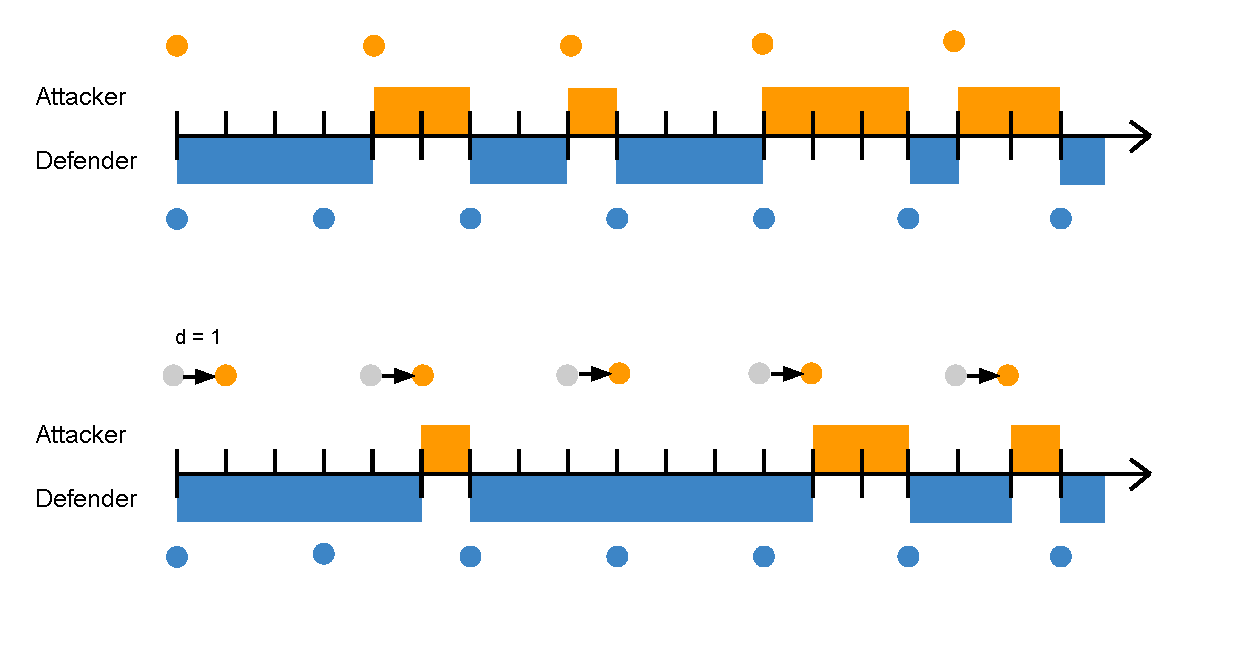
\includegraphics[scale=0.4]{../../doc/template/Images/FLipItCase1.pdf}
\label{fig:delaycase1}
\end{figure}


However, because of the delay required for virus propagation, the maximal time of control is reduced to $\delta_{D}-d$ , see figure \ref{fig:delaycase1}. There is a probability of \textit{r} that the attacker will move in the interval of the defender. However, the gain will not be half of the interval. Indeed, the attacker has to play soon enough to gain control, meaning that the attacker has to play during the period of $\delta_{D}-d$ during the interval of the defender. The probability that the attacker plays soon enough is $\dfrac{\delta_{D}-d}{\delta_{D}}$ and this will give the attacker an average gain of $\dfrac{\delta_{D}-d}{2}$. If the attacker moves after the period of $\delta_{D}-d$, the gain of the attacker will be zero. The probability that this happens is  $\dfrac{d}{\delta_{D}}$. The average gain rate of the attacker can then be expressed as follows if we look at one interval of the defender:
\begin{equation}\label{first}
\gamma_{A}(\alpha_{D},\alpha_{A}) = \dfrac {1}{\delta_{D}} [ \dfrac{\delta_{D}}{\delta_{A}} \cdot \dfrac{\delta_{D}-d}{\delta_{D}} \cdot \dfrac{\delta_{D}-d}{2} + \dfrac{\delta_{D}}{\delta_{A}} \cdot \dfrac{d}{\delta_{D}} \cdot 0 ]
\end{equation}

To derive the benefit, the cost of moving is subtracted from the average gain. 
\begin{equation}\label{first}
\beta_{A}(\alpha_{D},\alpha_{A}) = \dfrac { (\delta_{D}-d) ^{2}} {2 \cdot \delta_{D}  \delta_{A}} - k_{A} \alpha_{A}
\end{equation}
\begin{equation}\label{first}
\beta_{A}(\alpha_{D},\alpha_{A}) = \dfrac { \delta_{D}} {2 \cdot \delta_{A}} - k_{A} \alpha_{A} - ( \dfrac{d^{2}}{2 \cdot \delta_{A} \delta_{D}} - \dfrac{d}{\delta_{A}} )
\end{equation}
 
 
 The benefit of the defender is expressed as follows:
 \begin{equation}\label{first}
\beta_{D}(\alpha_{D},\alpha_{A}) = 1 - \dfrac { (\delta_{D}-d) ^{2}} {2 \cdot \delta_{D}  \delta_{A}} - k_{D} \alpha_{D}
\end{equation}
~~\\
We can easily see that when $d$=0, we obtain the formula of the original FlipIt game.\\


\subsection*{\textbf{Case 2:} $\delta_{A} \leq \delta_{D} $ (The attacker plays at least as fast as the defender.) }

First let $r = \dfrac{\delta_{D}}{ \delta_{A} }$. The intervals between two consecutive attacker's moves have length $\delta_{A}$. Consider a given attackers move interval. The probability over the attacker's phase selection that the defender moves in this interval is $\dfrac{\delta_{A}}{ \delta_{D} } = (1/r)$. Given that the defender moves within the interval of the attacker, he moves exactly once within this interval (since $\delta_{A} \leq \delta_{D} $) and his move is distributed uniformly at random. \\

A similar analysis as in case 1 for a FlipIt game without virus propagation yields the following benefits:

\begin{equation}\label{first}
\beta_{D}(\alpha_{D},\alpha_{A}) = \dfrac {1} {2r} - k_{D} \alpha_{D} = \dfrac {\delta_{A}} {2\delta_{D}} - k_{D} \alpha_{D} 
\end{equation}
\begin{equation}\label{first}
\beta_{A}(\alpha_{D},\alpha_{A}) =1 - \dfrac {1} {2r} - k_{A} \alpha_{A} = 1- \dfrac {\delta_{A}} {2\delta_{D}} - k_{A} \alpha_{A}  
\end{equation}\\


For the case with a virus we consider two cases, Case a and Case b, depending on whether the delay is shorter or longer than the difference between the attacker's and the defender's period.  \\


\subsubsection*{\textbf{Case a:} $d + \delta_{A} \leq \delta_{D}$}
~~\\
Consider a timespan $\delta_{A} + d$, representing the attacker's interval followed by the delay period in his next interval. The defender will never move twice during this timespan because $\delta_{A} + d \leq \delta_{D}$. The defender will move during the interval of the attacker with a probability of $\dfrac{\delta_{A}}{\delta_{D}} $. When this happens the defender will end with being in control at the end of the interval. In the next interval the attacker will have to regain control, meaning that during the delay, the defender stays in control, see figure \ref{fig:case2} cases (1) and (2). This means that the defender will keep the control over the resource in the next interval over a period of the delay, namely \textit{d}. Because $d + \delta_{A} \leq \delta_{D}$ the next move of the defender in this second interval will never occur during the delay, meaning that the entire delay can be considered as an extra benefit resulting of a play in the previous interval. 
So, every time the defender plays, he will get an average gain of $\dfrac{\delta_{A}}{2}$ in the interval where he plays and in the next interval will always receive a extra gain of $d$, yielding a total average gain per interval of
$\dfrac{(d+\dfrac{\delta_{A}}{2})}{\delta_{A}}$

The total gain  rate of the defender is then the probability that the defender will move during an interval of the attacker multiplied by the total average gain per interval: 

\begin{equation}\label{first}
\gamma_{D}(\alpha_{D},\alpha_{A}) = \dfrac{\delta_{A}}{\delta_{D}} \cdot \dfrac{(d+\dfrac{\delta_{A}}{2})}{\delta_{A}} 
\end{equation}
\begin{equation}\label{first}
\gamma_{D}(\alpha_{D},\alpha_{A}) = \dfrac{\delta_{A}}{2\delta_{D}} + \dfrac{d}{\delta_{D}} 
\end{equation}\\
This yields in the following benefit formula:
\begin{equation}\label{first}
\beta_{D}(\alpha_{D},\alpha_{A}) = \dfrac{\delta_{A}}{2\delta_{D}} + \dfrac{d}{\delta_{D}} - k_{D} \alpha_{D} 
\end{equation}\\

The benefit for the attacker will be as follows:
\begin{equation}\label{first}
\beta_{A}(\alpha_{D},\alpha_{A}) = 1 -\dfrac{\delta_{A}}{2\delta_{D}} - \dfrac{d}{\delta_{D}} - k_{A} \alpha_{A} 
\end{equation}\\

\begin{figure}[hbtp]
\caption{Case 2 where d + deltaA < deltaD}
\centering
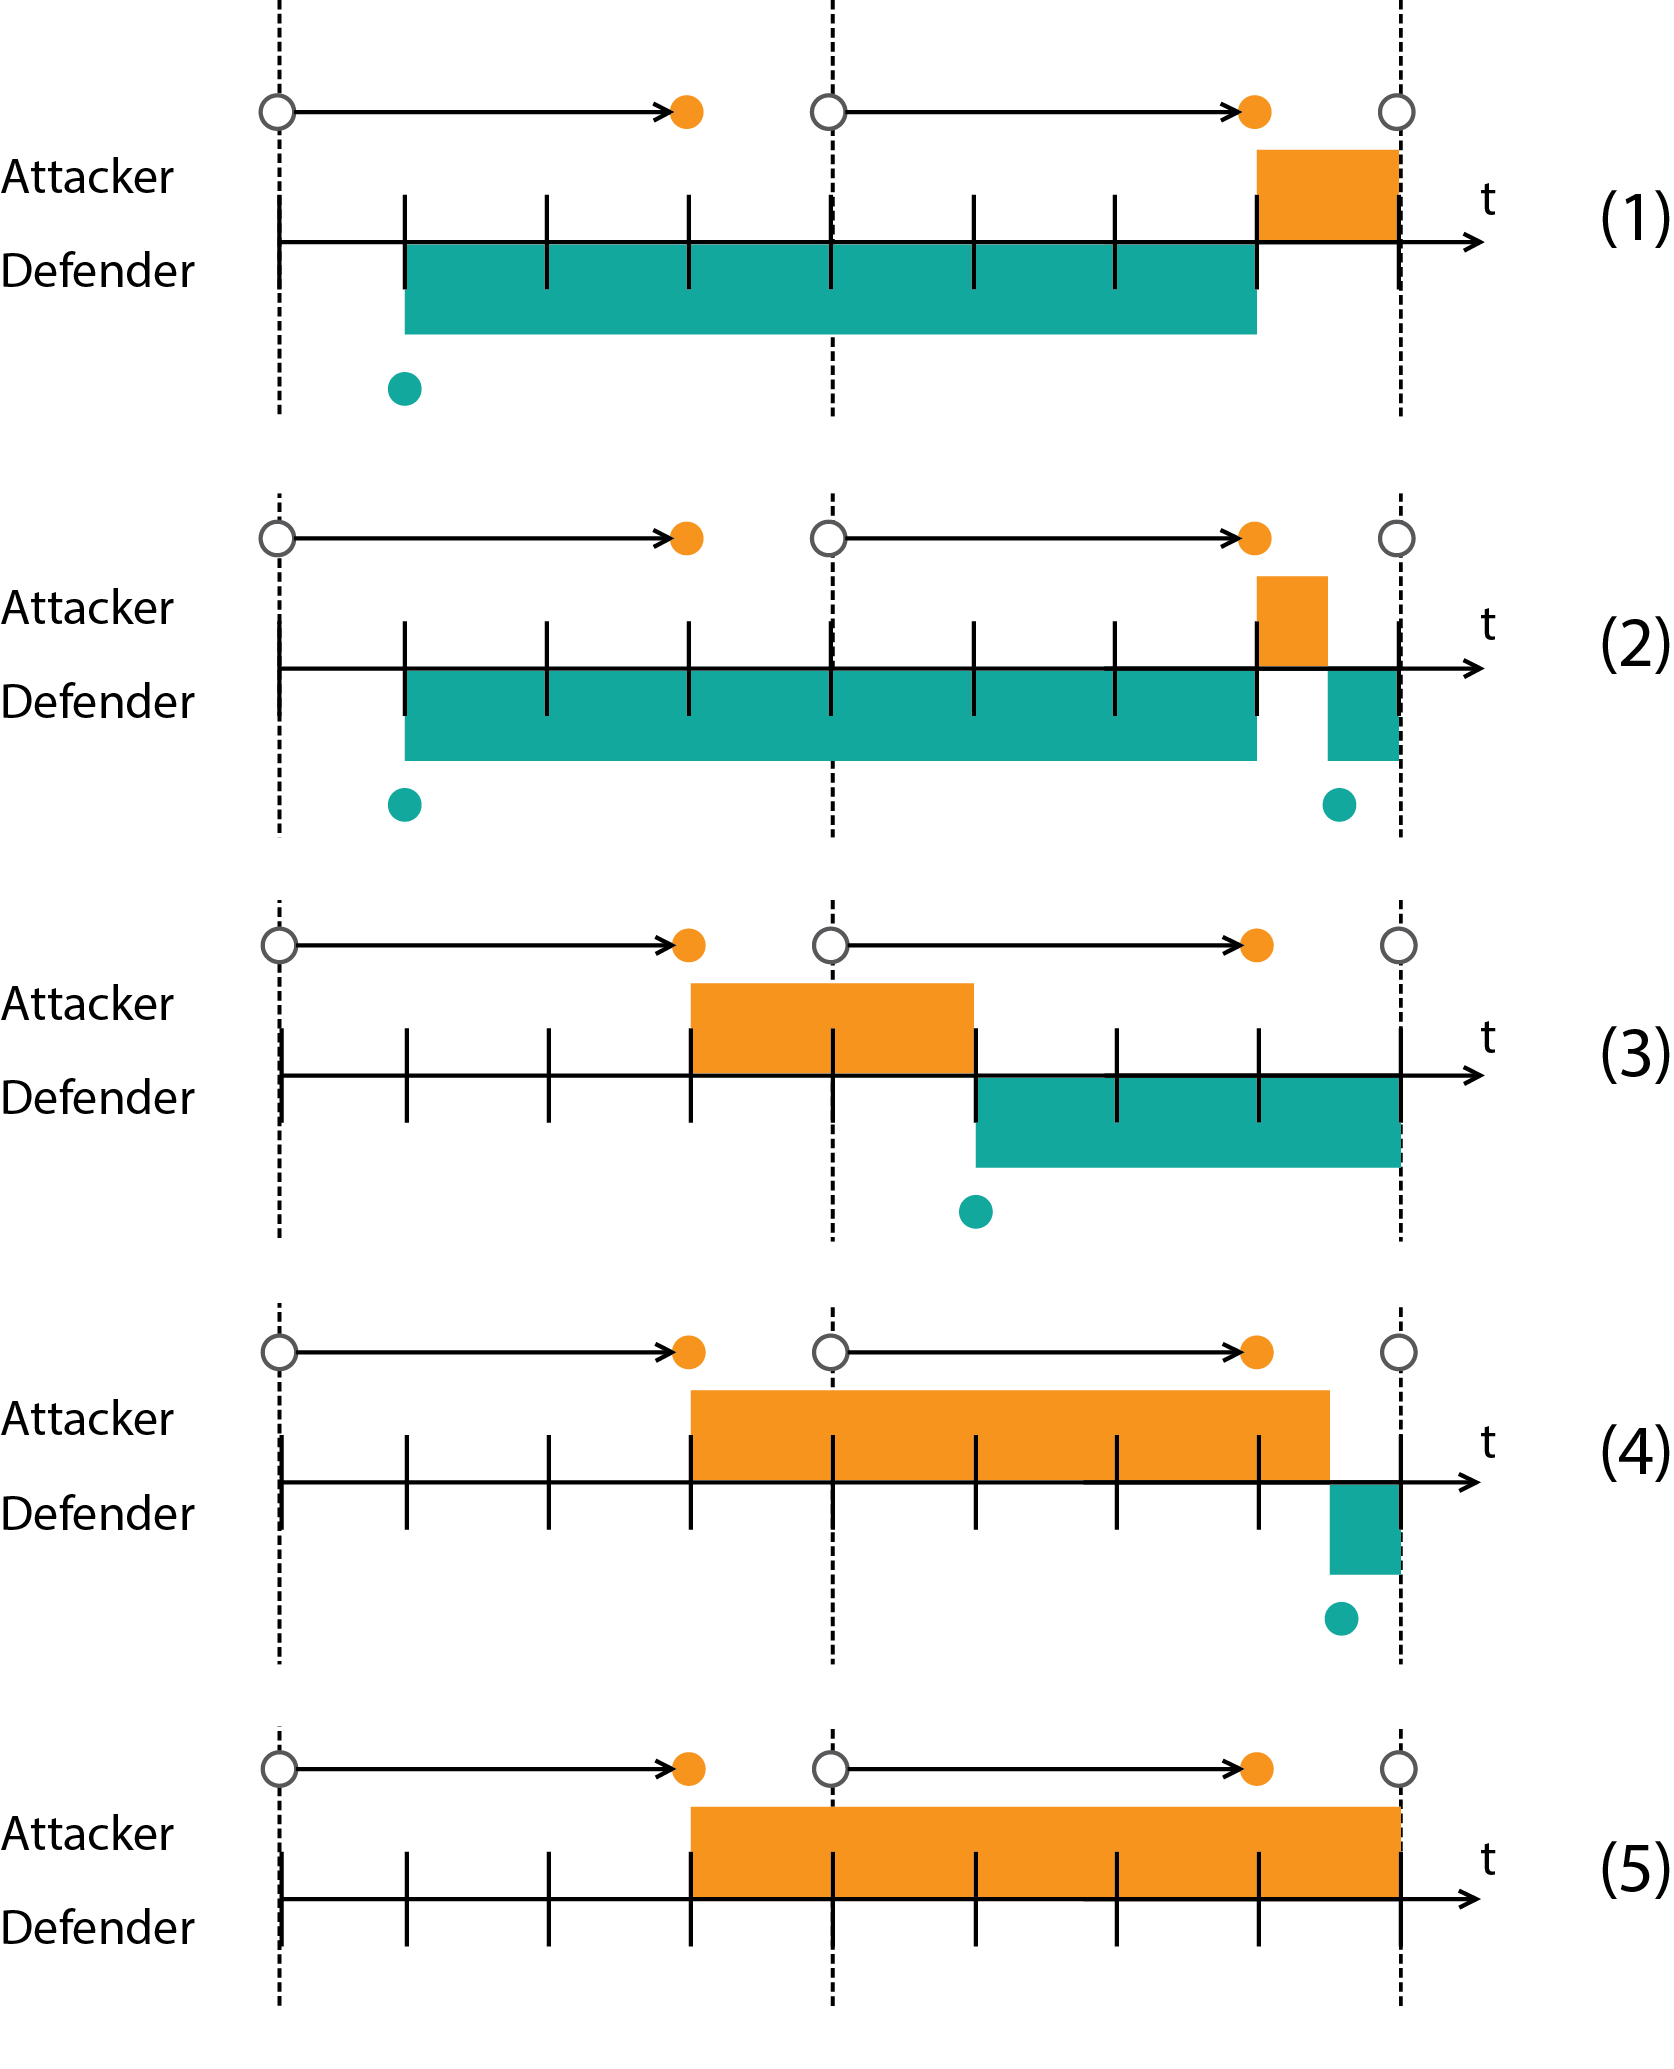
\includegraphics[scale=0.5]{../../doc/template/Images/FlipItCase2.png}
\label{fig:case2}
\end{figure}


It is crucial that $ \delta_{D}$ is at least as large as $d + \delta_{A}$. If not, this would mean that the defender can move during the delay in the interval following the interval where the defender already moved. This would mean that there can be an overlap between the average gain of $\dfrac{\delta_{A}}{2}$ and the delay. The above benefit formula would then include to much gain for the defender: the potential overlap during the delay would be counted twice. \\


~~ \\
\subsubsection*{\textbf{Case b:} $d + \delta_{A} \geq \delta_{D}$}
~~~\\

To obtain the formula in case of a too long delay, we therefore need to subtract this overlapping gain from the above formula. 
Since $\delta_{D} \geq \delta_{A}$, if the defender enters the interval immediately after the attacker has played, then the defender cannot have played in the previous interval. In that case, there is no overlap. So the problem of the overlap only appears if the defenders enters late enough and thus only the last part of the delay is subject to overlap. The larger the difference between the interval of the defender and the attacker, the smaller the risk of overlap. Concretely, only the last part of length $d - (\delta_{D} - \delta_{A})$ is subject to overlap. Hence, the probability of overlap is $\dfrac{ d - (\delta_{D} - \delta_{A})}{\delta_{D}}$ and the gain will be half of this interval:  $\dfrac{ d - (\delta_{D} - \delta_{A})}{2}$.  The gain rate to be subtracted is therefore:\\

\begin{equation}\label{first}
\dfrac{1} {\delta_{A}} \cdot \dfrac{d - (\delta_{D} - \delta_{A})}{\delta_{D}} \cdot \dfrac{d - (\delta_{D} - \delta_{A})}{\delta_{D}}
\end{equation}

The total gain  rate of the defender is obtained by subtracting this term from the gain rate of case a:
 \begin{equation}\label{first}
\gamma_{D}(\alpha_{D},\alpha_{A}) = \dfrac{\delta_{A}}{\delta_{D}} \cdot \dfrac{(d+\dfrac{\delta_{A}}{2})}{\delta_{A}} - \dfrac{(d - (\delta_{D} - \delta_{A}))^{2}}{2 \delta_{D} \delta_{A}}
\end{equation}
\begin{equation}\label{first}
\gamma_{D}(\alpha_{D},\alpha_{A}) = \dfrac{\delta_{A}}{2\delta_{D}} + \dfrac{d}{\delta_{D}} - \dfrac{(d - (\delta_{D} - \delta_{A}))^{2}}{2 \delta_{D} \delta_{A}}
\end{equation}\\
This yields in the following benefit formula:
\begin{equation}\label{first}
\beta_{D}(\alpha_{D},\alpha_{A}) = \dfrac{\delta_{A}}{2\delta_{D}} + \dfrac{d}{\delta_{D}} - k_{D} \alpha_{D} - \dfrac{(d - (\delta_{D} - \delta_{A}))^{2}}{2 \delta_{D} \delta_{A}}
\end{equation}\\
 
The benefit for the attacker will be as follows:
\begin{equation}\label{first}
\beta_{A}(\alpha_{D},\alpha_{A}) = 1 -\dfrac{\delta_{A}}{2\delta_{D}} - \dfrac{d}{\delta_{D}} - k_{A} \alpha_{A} + \dfrac{(d - (\delta_{D} - \delta_{A}))^{2}}{2 \delta_{D} \delta_{A}}
\end{equation}\\


\section{Nash Equilibrium}
Verder door schrijven

\section{Conclusions and Further Research}
\label{ch:conclusion}
In this paper we presented an adaptation of the FlipIt game to the situation of virus propagation, such as to take the delay for network infection into account. We discerned two cases. In the case the defender plays faster than the attacker, the attacker simply looses the delay. In the case the attacker plays faster, each time the defender plays in an interval, he will gain extra time of the delay. The delay is therefore always detrimental to the benefit of the attacker. 
This demonstrates that the FlipIt game can be adapted to a game with virus propagation. Further research needs to be performed to calculate the impact of the delay on Nash equilibria and the determination of optimal defender and attacker strategies.
%In dit \textit{abstract} environment wordt een al dan niet uitgebreide
%Nederlandse samenvatting van het werk gegeven.
%Wanneer de tekst voor een Nederlandstalige master in het Engels wordt
%geschreven, wordt hier normaal een uitgebreide samenvatting verwacht,
%bijvoorbeeld een tiental bladzijden. \\
%  
%Dit is het kort geschreven.\\ Eigenlijk paper in het nederlands schrijven \\
%Intro -- positionering -- vraagstelling -- oplossingen en contributies \\
%Flipit en cybersecurity\\
%Flipit met delay \\
%Berekeningen \\
%Niet zo lang geleden werden APT's ontdekt. (Introzin moet beter en anders). Bedrijven worden door APTs aangevallen. Belangrijk om APTs tegen te gaan. Geven een grote kost aan de bedrijven. Hun stealthy aspect is vervelend en moeilijk aan te pakken. Preventie is beter dan detectie. Eens ze binnen zijn kunnen we veel schade veroorzaken. Conventionele middelen zoals firewalls, malware detection helpen hier niet tegen. Nieuwe methode nodig. Gametheory FlipIt. FlipIt uitleggen. Deze formules gaan we dan omvormen tot ze wel propagatie delay kunnen modelleren. Hiervan berekenen we ook het Nash equilibrium. 
\end{abstract*}

% Een lijst van figuren en tabellen is optioneel
%\listoffigures
%\listoftables
% Bij een beperkt aantal figuren en tabellen gebruik je liever het volgende:
\listoffiguresandtables
% De lijst van symbolen is eveneens optioneel.
% Deze lijst moet wel manueel aangemaakt worden, bv. als volgt:
\chapter{List of Abbreviations and Symbols}
\section*{Abbreviations}
\begin{flushleft}
  \renewcommand{\arraystretch}{1.1}
  \begin{tabularx}{\textwidth}{@{}p{12mm}X@{}}
    RSA & Rivest-Shamir-Adleman \\
    DDoS & Distributed Denial of Service \\
    APT & Advanced Persistent Threat \\
    CIA & Confidentiality , Integrity and Availability \\
    USB & Universal Serial Bus \\
    NA & Non-Adaptive \\ 
    AD & Adaptive \\
    LM & Last Move \\
    FH & Full History \\
    VM & Virual Machine \\
    IP & Internet Protocol \\
    DNS & Domain Name System \\
    BGP & Border Gateway Protocol \\
    SEM & Simple Epidemic Model \\
    SI & Susceptible - Infected \\
    SIR & Susceptible - Infected - Recovered \\
    SIS & Susceptible - Infected - Susceptible \\
    OSN & \\
    AAWP & \\
      \end{tabularx}
\end{flushleft}
\section*{Symbols}
\begin{flushleft}
  \renewcommand{\arraystretch}{1.1}
  \begin{tabularx}{\textwidth}{@{}p{12mm}X@{}}
 $i$ & $i \in \{D,A\}$, defines the player. `D' is the defender and `A' is the attacker. \\
 $\delta_{i}$ & The length of the interval between two consecutive moves of player \textit{i}. \\
 $\alpha_{i}$ & The average flip rate of player \textit{i}, given by $\alpha_{i}=1/\delta_{i}$. \\
$k_{i}$ & The cost of player \textit{i}'s moves. \\
$d$ & The delay caused by the propagation of a threat. \\
 $G_{i}(t)$ & The total gain of player \textit{i} denotes the amount of time player \textit{i} is in control over the resource up to time \textit{t}. \\
$\gamma_{i}$ & The average gain rate of player \textit{i} defined as $G_{i}(t)/t$. \\
$\beta_{i}$ &  The average benefit rate up to time \textit{t} defined as  $\beta_{i} = \gamma_{i} -k_{i} \alpha_{i} $. \\
$opt_{i}$ & The optimum function. \\
$n_{i}(t)$ & The amount of moves made by player \textit{i} up to time \textit{t}. \\
  \end{tabularx}
\end{flushleft}

% Nu begint de eigenlijke tekst
\mainmatter

%\chapter{Introduction}
\label{cha:intro}
The first contains a general introduction to the work. The goals are
defined and the modus operandi is explained.

\section{chap}

%%% Local Variables: 
%%% mode: latex
%%% TeX-master: "thesis"
%%% End: 

\chapter{Introduction}
\label{cha:10}
%\documentclass[10pt]{article}
%\begin{document}

%%%%%%%%%%%%%%%%%%%%%%%%%%%%%%%%%%%%%%%%%%%%%%%%%%%%%%%%%%
%%%%%			Introduction Chapter 10			%%%%%%
%%%%%												%%%%%%
%%%%%												%%%%%%
%%%%%%%%%%%%%%%%%%%%%%%%%%%%%%%%%%%%%%%%%%%%%%%%%%%%%%%%%%

\section{Introduction}

In this era where digitalization becomes prominent in every aspect of our lives, where technology is growing fast and where businesses are always under attack, security becomes an issue of increasing complexity. Security is needed to protect websites, servers, applications, data, operating systems and other assets that need protection in a computer network. Without security, there is no protection to keep somebody out of a system. It is the same as leaving the door of your house wide open for everyone to come in. \\
%Businesses can have confidential information on clients. Through data leakage, confidential information can be lost and possibly used by the competitor. Businesses wants to meet their service-level agreements. They will protect themselves against disruption that can be caused by DOSS attacks. Ultimately, system and network security helps protecting a business's reputation, which is one of its most important assets. 

Why is it so important to keep a system secure?  Many businesses store confidential information, which can be lost through data leakage and can possibly be abused by competitors. Also, disruption caused by distributed denial of service (DDoS) attacks, may result in businesses failing to meet their service-level agreements. Ultimately, computer and network security helps protecting a business against various kind of threats. \\
%\todo{waarom?  :  lekken van informatie: je hebt info over klanten en moet hun privacy beschermen, je eigen data is geld waard voor concurrenten, DOSS attacks: je will je service-level agreements kunnen nakomen, ..}
% A hacker will be a person that seeks exploits or weaknesses in a system or network in order to gain access.  Many of those attacks have a different cause. Some of the attacks by a hacker can be benign, others can be harmful. There are various ways to break into a system. Viruses, worms, spyware and other malware are the number two of the top external threats that a business faces [security report kaspersky 2014]. (number one is Spam). Furthermore these kind of threats also causes the greatest percentage in loss of data. These threats will infect the network by means of a virus that will propagate through the network. Most of the attacks are Advanced Persistent Threats (APT).\\

A particular kind of threat is an Advanced Persistent Threat (APT). An APT is a multi-faceted, continuous and targeted cyber attack that is designed to penetrate a network or a system in a stealthy way and can stay undetected for a long period of time. It is different and more severe than a conventional threat. A conventional threat will not attack any particular target. An APT is persistent and will keep on trying to attack its victim. It operates silently and stealthily, to prevent detection. This makes it so hard to protect a network or a system against an APT. 

%Bruce Schneier describes an APT as something different and stronger than a conventional threat: ''\textit{A conventional hacker or criminal is not interested in any particular target. He wants a thousand credit card numbers for fraud, or to break into an account and turn it into a zombie, or whatever. Security against this sort of attacker is relative; as long as you're more secure than almost everyone else, the attackers will go after other people, not you. An APT is different; it's an attacker who - for whatever reason - wants to attack you. Against this sort of attacker, the absolute level of your security is what's important. It does not matter how secure you are compared to your peers; all that matters is whether you're secure enough to keep him out}'' - Bruce Schneier \cite{APTBruce}.\\


%\subsubsection{Complication}
%Since it is so difficult to protect a system or a network against APT's, researchers have been looking for effective ways to predict in advance which defence strategy might be the better one. 
There are a number of key strategies an organisation can apply to defend itself against APTs: awareness, whitelisting, system administration, network segregation, dynamic content checking and patch management. Nevertheless the combination of all these elements benefits from being complemented by other defence strategies to protect oneself against stealthy takeovers. One possible way to study the impact of stealthy takeovers and to determine practical recommendations for defenders is through game theory.\\
Game theory is gaining increasing interest as an effective technique to model and study cyber security problems. It is common to model cyber security problems as a game with two players, an attacker and a defender. There are, however, games that have more players e.g. when a third party is involved \cite{fengstealthy}. This paper focusses on a game with two players. The actions available to the attacker and the defender correspond respectively to the attacks on the system and the defensive measures that protect the system. \\

Many security games that bridge the gap between game theory and cyber security have already been investigated, so finding a new game can be challenging. This paper builds on a relatively new paper where the assumption of stealthiness is fairly unique, giving some interesting results.\\ 
 The paper is from researchers at RSA, van Dijk et al,  who presented a game-theoretic framework to model computer security scenarios called ``FlipIt'' \cite{FlipIt}. They study the specific scenario where a system or network is repeatedly taken over completely by an attacker. This take-over is not immediately detected by the defender. It is a two-player game where the attacker and the defender are competing to get control over a shared resource. Neither player knows who is currently in control of the resource until they move. In FlipIt every move involves a cost and gives them immediate control over the resource. The attacker will try to maximise the time that he controls the network, while the defender will try to maximise the time that the network is free of malware. \\
 But what if the attacker moves and it takes some time before the attacker gets full control over the resource? FlipIt does not take into account that a move may not be instantaneous, but has a certain delay. Consider for example a network with different nodes (laptops, datacenters) as a resource. The attacker drops a virus on one of the nodes and waits until this virus infects the whole network. The attacker will only be in control of the resource when a sufficiently large amount of nodes of the network are infected. In this paper we present an adaptation of FlipIt to model a game where the moves of the attacker are not instantaneous. The formalization for this game starts from the model of non-adaptive continuous basic FlipIt game where players use a periodic strategy with a random phase.   \\

\subsubsection{Research questions}

%This paper proposes the adaptation of the FlipIt formulas as presented in \cite{FlipIt} such as to take the delay for virus propagation into account. In the next section we first present the original FlipIt game. Then section \ref{ch:flipitvirus} presents the FlipIt game with virus propagation. Section \ref{ch:extendedWork} presents some related work. Section \ref{ch:conclusion} concludes the paper and presents avenues for further research.

This paper adapts the model presented in \cite{FlipIt} so as to take the delay for virus propagation into account.
This leads us to the following research questions:
\begin{itemize}
\item How can we incorporate the notion of delay in the game-theoretical analysis of the FlipIt game for a periodic strategy?
\item Does the resulting model allow an optimal defence strategy against an attacker? 
\end{itemize}

\subsubsection{Contributions and results}
The following contributions are made in this paper:
\begin{itemize}
\item[-] We propose an addition to the basic FlipIt model to model a scenario where the moves by the attacker will not be instantaneous. We extend the FlipIt game to a game wherein the attacker flips with a delay. The attacker only compromises the system if sufficient nodes in the network are infected. 
\item[-] The periodic case of FlipIt is modelled with a delay, resulting in optimum functions and Nash equilibria. \todo{punt herschrijven en meer nadruk leggen op het vinden van de Nash equilibria}
\item[-] Based on our results we can give practical recommendations to take measures against advanced attacks.  The modelling of FlipIt with a propagation delay will give a guideline for both the attacker and the defender on how to respectively plan attacks or network clean-ups.
\item[-] This work includes an overview of different propagation techniques of worms and models used to calculate the propagation delay (depending on the network layout). It also presents a method to calculate the speed of the propagation of a worm in a propagation independent of the topology of the network.
\item[-] The Google Page Rank matrix is introduced as a proof of concept to calculate the importance of every node in the network.
\end{itemize}


While it may seem trivial to extend the basic FlipIt model with a propagation delay, its mathematical treatment is not. In the paper of Laznka et all. \citep{FlipThem} it seems that even a small extension adds to the already significant mathematical complexity. Even though the FlipIt game is quite symmetric, the mathematical complexity rises by adding a propagation delay.
% First a formula to calculate the benefit of a basic FlipIt was derived to introduce the propagation delay. To calculate the benefit for each case depending on the periods of the attacker, defender and the delay, the intervals where not independent any more as in the basic FlipIt game. The previous intervals had to be taken into account to calculate the benefit of the players in its own interval. 

%\subsubsection{Conjunctures and open problems}
%
%\begin{description}
%\item[-] Analyse other strategies like renewal strategies instead of only periodic strategies.
%\item[-] The defender can chose to Flip one node of the network or a subset instead of all the nodes.
%\item[-] Give the defender a delay. It takes a while before a patch is made after the discovery of a vulnerability.
%\end{description}

\subsubsection{Overview of the thesis}

The organisation of this paper is the following.  An introduction to cyber security and game theory is given in chapter \ref{Chapter1:Intro.Game.Theory} to allow the reader to become familiar with the kind of threats that are in the scope of this work and the game theoretic concepts that will be further used in the paper. In the same chapter the FlipIt framework is summarized with its most important conclusions. The chapter concludes with an overview of the related work on FlipIt and further clarifies the contributions of this paper compared to existing work. 
Chapter \ref{chapter2:FlipIt with virus propagation} first introduces the adaptations made to the original FlipIt game to model a FlipIt game with a virus propagation delay. Subsequently formulas are derived to model a FlipIt game with a propagation delay for the specific case where players play a periodic strategy with a random phase. \\
In Chapter \ref{chapter:Nash} the formulas are further analysed to determine if there is a Nash equilibrium. 
In order to provide a clear perspective on delays, chapter \ref{chapter4: Worm propagation} gives an overview of the various methods of propagation and worm propagation models. It presents a method to calculate the speed of the propagation of a worm in a network independent of the topology of the network.
Finally chapter \ref{chapter5:conclusion} discusses the main results and provides directions for further research.


%In this paper we want to focus on situations where a computer network is attacked by an APT. These threats will infect the network by means of a virus that will propagate through the network. 
%ð  Dat is geen vraag.
%
% 
%Kijk naar de opdracht van je thesis. De vraag zou bv. kunnen zijn:
%General research question: Does the application of game theory help in defining a good defense (or attacker) strategy ?
%This question is to large, so we reduce the question to …
%Specific research question:
%-         Is it possible to incorporate the notion of delay in the game-theoretical analysis of the Flip-It game ?
%
%-        Can we calculate a Nash Equilibrium for a FlipIt Game with delay ?
%
%-        Does this allow us to determine an optimal defense strategy against an attacker ?
%
% 
%Je matrix-berekening beantwoordt de vraag:
%-        How can we calcuate the expected duration for a node’s infection/the entire network infection ?
%
%-        Can we calculate this node per node ?
%
% 
%Complication
%Wat je schrijft is veel te algemeen. Maak het heel concreet en toegespitst op jouw specifieke bijdrage ?
%ð  De complicatie is dat de FlipIt game geen rekening houdt met de delay


%%%% Local Variables: 
%%%% mode: latex
%%%% TeX-master: "thesis"
%%%% End: 


%gebruik van mijn model kan bevoorbeeld gebruikt worden om aan te duiden hoe vaak paswoorden moeten worden veranderd. 

%\chapter{Intoduction to GameTheory}
\label{cha:1}
%\documentclass[10pt]{article}
%\begin{document}

%%%%%%%%%%%%%%%%%%%%%%%%%%%%%%%%%%%%%%%%%%%%%%%%%%%%%%%%%%
%%%%%			Introduction Chapter 1				%%%%%%
%%%%%												%%%%%%
%%%%%												%%%%%%
%%%%%%%%%%%%%%%%%%%%%%%%%%%%%%%%%%%%%%%%%%%%%%%%%%%%%%%%%%

In the following paragraph an introduction to game theory is given based on the work of \todo{werk van Essentials of Game Theory} and \todo{Coursera game theory}. Voor een meer gedetailleerdere intro ook dit boek. .
%------------------------------------------------%
%            Intro Game Theory 					 %
%------------------------------------------------%
\section{Intro Game Theory}
\label{Cha:1:Intro.Game.Theory}

%begin over dat gametheorie handig is in de economie
Game theory studies the interaction between independent and self-interested agents. It is a mathematical way of modelling the interactions between two or more agents where the outcomes depend on what everybody does and how it should be structured to lead to good outcomes. For this reason it is very important for economics and also for politics, biology, computer science, philosophy and a variety of other disciplines.  \\
%Every agent has different levels of happiness for the different outcomes.
%self interested meaning

One of the assumptions underlying game theory is that the players of the game, the agents, are independent and self-interested. This does not necessarily mean that they want to harm other agents or that they only care about themselves. 
%utility function meaning 
Instead it means that each agent has preferences about the states of the world he likes. These preferences are mapped to natural numbers and are called the utility function. The numbers are interpreted as a mathematical measure to tell you how much an agent likes or dislikes the states of the world. \\
It also explains the impact of uncertainty. When an agent is uncertain about a distribution of outcomes, his utility will describe the expected value of the utility function with respect to the probability of the distribution of the outcomes. For example: with 0.7 probability it will be 7 degrees outside and 0.3 probability it will be 10 degrees. The agent can have a different opinion about that distribution versus another distribution. (\todo{uitleggen aan de hand van een voorbeeld}).\\
%Cooperative and non cooperative games
In a decision game theoretic approach an agent will try to act in such a way to maximise his expected or average utility function. It becomes more complicated when two or more agents want to maximise their utility and whose actions can affect each other utilities. This kind of games are referred to as non cooperative game theory, where the basic modelling unit is the group of agents. The individualistic approach, where the basic modelling is only one agent, is referred as cooperative game theory. 

There are two standard representations for games. The first one is the Normal Form. The second one is the Extensive Form.

In the following list a couple of terms that will be used throughout the paper.
\begin{description}
\item \textit{Players}: players are referred as the ones who are the decision makers. It can be a person, a company or an animal.
\item \textit{Actions}: actions are what the player can do. 
\item \textit{Outcomes}:  
\item \textit{Utility function}: the utility function is the mapping of the level of happiness of an agent about the state of the world to natural numbers.
\item \textit{Strategies}: A strategy is the combination of different actions. A pure strategy is only one action.
\end{description}

A game in game theory consists of multiple agents and every agent has a set of actions that he can play. 



%Nash equilibrium



% --------------- example of a game -----------------%


\section{Other}
In this chapter an introduction to gametheory will be given with the formulas that will be used troughout this paper. We start with the basics of gametheory. People that have a background in gametheory can skip this chapter.
%------------------------------------------------%
%            Intro about virusses				 %
%------------------------------------------------%
\section{Virusses}

Many network security threats today are spread over the Internet. The most common include:

Viruses, worms, and Trojan horses
Spyware and adware
Zero-day attacks, also called zero-hour attacks
Hacker attacks
Denial of service attacks
Data interception and theft
Identity theft

%http://www.ists.dartmouth.edu/library/258.pdf Email Virus Propagation Modeling and Analysis
%Cliff C. Zou∗, Don Towsley†, Weibo Gong∗
%∗Department of Electrical & Computer Engineering
%†Department of Computer Science
%Univ. Massachusetts, Amherst
%Technical Report: TR-CSE-03-04

Computer virus through mail. 
Though virus spreading through email is an old technique, it is still effective and is widely used by
current viruses and worms. Sending viruses through email has some advantages that are attractive to
virus writers:
 Sending viruses through email does not require any security holes in computer operating systems
or software.
 Almost everyone who uses computers uses email service.
 A large number of users have little knowledge of email viruses and trust most email they receive,
especially email from their friends [28][29].
 Email are private properties like post office letters. Thus correspondent laws or policies are required
to permit checking email content for detecting viruses before end users receive email [18].

Send a email with malicious attachment. Only again infected if attachment again opened. Thus this is the action of attacking every neighbour node + also can attack again the node where the virus was coming from.
There are also email viruses were the malicious program is hidden in the txt and the attachment does not need to be opened. 

%http://www.cisco.com/web/offer/gist_ty2_asset/Cisco_2014_ASR.pdf p49
%http://repo.hackerzvoice.net/depot_madchat/vxdevl/papers/avers/2004-35.pdf
%http://www.mcafee.com/us/resources/white-papers/foundstone/wp-managing-malware-outbreak.pdf


\subsection{What are my topics}
\begin{itemize}
\item Security, Costs, Cybersecurity
\item Viruses, kinds
\item Gametheory
\item Flip-it
\item Flip-it multiple resources
\item 
\end{itemize}

\subsection{Malware}
%Does a company network faces lot of malware? what is the cost ?
Relevant researches:
\begin{itemize}
%http://ants.iis.sinica.edu.tw/3BkMJ9lTeWXTSrrvNoKNFDxRm3zFwRR/17/04483668.pdf
\item How Viruses and worm can be detected. Difference between UDP en TCP worm propagation
\end{itemize}




%%%%%%%%%%%%%%%%%%%%%%%%%%%%%%%%%%%%%%%%%%%%%%%%%%%%%%%%%%
%%%%%			Conclusion Chapter 1				%%%%%%
%%%%%												%%%%%%
%%%%%												%%%%%%
%%%%%%%%%%%%%%%%%%%%%%%%%%%%%%%%%%%%%%%%%%%%%%%%%%%%%%%%%%
\section{Conclusion}
\label{Cha:1:Conclusion}
The final section of the chapter gives an overview of the important results
of this chapter. This implies that the introductory chapter and the
concluding chapter don't need a conclusion.


%%% Local Variables: 
%%% mode: latex
%%% TeX-master: "thesis"
%%% End: 

%\end{document}

\chapter{Intoduction to GameTheory}
\label{Chapter1:Intro.Game.Theory}
%\documentclass[10pt]{article}
%\begin{document}

%%%%%%%%%%%%%%%%%%%%%%%%%%%%%%%%%%%%%%%%%%%%%%%%%%%%%%%%%%
%%%%%			Introduction Chapter 1				%%%%%%
%%%%%												%%%%%%
%%%%%												%%%%%%
%%%%%%%%%%%%%%%%%%%%%%%%%%%%%%%%%%%%%%%%%%%%%%%%%%%%%%%%%%

This chapter provides the reader with an introduction to the general context of the work presented in this paper.  Section 2.1 introduces the reader into the basic concepts of cyber security and the kind of cyber security threaths that are in the scope for this work. Section 2.2 then introduces the reader into the main principles of game theory. Subsequently, section 2.3 introduces the reader to the FlipIt game, the specific game that will be used to model cyber security attacks of periodic nature and including a delay.  Finally, section 2.4 gives an overview of the related work, and how the research presented in this thesis is positioned compared to existing results.

\section{What is cyber security?}

Before the digitalization of documents, information was kept on paper and the security of this information was ensured by administrative and physical means. For example, you needed a key to access documents stored in a room full of cabinets where the files were kept. In today's digital era more and more information is kept in a digital format, stored on a computer.  As digitalization progressed, the need for ensuring the security of digital information arose and automated tools where developed for protecting files stored on a computer.  The generic name to protect data stored on a computer controlled device such as computers and smartphones, as well as public and private computer networks, including the entire Internet is called computer security. 
Security is a general term that encompasses several dimensions. More specifically, computer security has tree key objectives that are fundamental to computer security:

~~\\
 \textit{Confidentiality}: This assures that the confidential of private data is not disclosed or made available to users that do not have the authorization. \\
 \textit{Integrity:} This assures that data can not be altered by an unauthorized individual.\\
 \textit{Availability:} This assures that data is always accessible and that the service is not denied to authorized individuals.\\


 %The purpose of security is to give certainty that data will not be removed without authorization (Confidentiality) that the data is always accessible (Availability), and that data can not be read or altered by someone who does not have the authorization (Integrity). 
 These are the 3 key attributes of security, also known as the CIA triad. The tree concepts are fundamental security objectives for the securing of data, information and computing services. \\
Cyber security is the process of applying security tools to ensure confidentiality, integrity, and availability of data. It is an attempt to protect websites, servers, data, applications, operating systems and all assets that need protection in a computer system.  Some of these tools may include detection, identification or removal tools. A detection tool will determine if an infection has taken place and will trace the threat. An identification tool will try to identify the threat to be able to know how to remove it. The removal tool will once the threat has been identified, remove the threat from the system so that it cannot spread any further. 

%Cybersecurity attempts to ensure the protection of assets, which includes data, desktops, servers, buildings, and most importantly, humans. The goal of cyber security is to protect data both in transit and at rest. Countermeasures can be put in place in order to increase the security of data. Some of these measures include, but are not limited to, access control, awareness training, audit and accountability, risk assessment, penetration testing, vulnerability management, and security assessment and authorization.'' \todo{tekst overgenomen van wikipedia} \\

\subsubsection{Threats to computer systems}


In order to keep a system secure and to be able to apply security tools, it is important to mitigate the possible threats. The possible threats can take many forms, the most common being spam, malware, spoofing, phishing and  DDoS attacks.  In the context of cyber security, the terms ' threat and attack' are often used interchangeably, referring to more or less the same thing. They however have a slightly different meaning. A threat refers to anything that can breach the security and that can cause a possible harm. It is a possible danger that can exploit a vulnerability. An attack is an assault on computer security that comes from a threat. It is an intelligent act that tries deliberately to breach security through vulnerabilities.  \\

The most noteworthy group and biggest group of threats to computer systems is malware. 
This is a piece of malicious software that is designed to penetrate unprotected systems or computers, with the intent to get sensitive information, destroy data, or compromise the confidentiality, integrity or availability of the data or applications of the victim. A security report of 2014 \cite{SurveyKaspersky} reveals that 61\% of the attacks on companies are caused by malware. For this reason this section will examine the categories of malware threats. Different types of malware exist such as virusses, worms, flooders, rootkits, bots, spyware, adware and many more. This broad range of different types can be classified into two main categories, the first one based on the propagation method that is used and the second one for the payload or the variety of actions that the malware performs. Propagation methods include virusses, worms and trojans. Payload includes flooders, rootkits, bots, spyware and adware. In this paper we focus on the category of propagation methods and not on the actions that the malware performs. We give a brief explanation of the three main propagation methods of malware. \todo{opsplitsing uit het boek van network security genomen}


\begin{description}
\item \textit{Virus}: This is a malicious piece of code that replicates itself and tries to spread in order  to infect other systems or files. A typical virus will attach itself to a program, or an executable content on a computer. The ''I love you'' virus is an example of a virus where the virus attached itself as an executable to a mail. To propagate it used the mail systems. If someone opens an email with the "I love you"  in the annex, the virus will spread itself by sending a mail to everyone in the victim's contact list. So the virus can multiply rapidly and eventually a business network might shut down by the heavy traffic. In this example, there is a need for human interaction to spread the virus. If no one opens the mail the virus can not spread itself and infect other systems.

\item \textit{Worm:} A worm is a virus that can spread without human interaction. A worm is a computer program that replicates itself in order to spread to other hosts on a network. Copies of the worm can be forwarded via a computer network without an intermediary. The worm will use vulnerabilities of the system to infect other computers.
The Stuxnetworm is a very prominent example of a worm. Initially this worm was spread via infected USB sticks and from there it could spread itself without any further human intervention through the Internet to other hosts on the network. The purpose of the Stuxnetworm was to harm the centrifuges in nuclear reactors and many reactors have been infected.  

\item \textit{Trojan:} This is a malicious program that disguises itself as something normal and useful, so that users won't be suspicious of installing it, but it has a malicious function hidden inside that can avoid security measures and cause harm.  A notable trojan horse is Koobface, that targeted users of facebook, skype, yahoo, gmail and AOL mail. To spread itself the worm sended a mail or friend request with a message that directed the recipients to another third party website. This site tried to put the reciepient into downloading an update of Adobe Flash Player. Once downloaded and executed, Koobface could infect the host. 

\end{description}

A company can take different measures to defend itself against malware. The threats caused by malware can be divided into three main categories: known threats (70\%), unknown threats (29\%) and advanced threats (1\%) as proposed by Kasperksy \cite{APTKaspersky}. 

The known threats are the easiest to defend oneself against. Standard malware protection tools like firewalls and virus scanners can keep these kind of malware out of the system. Installing protection against unkown is also relatively easy, but this will need tools that go beyond the standard methods like dynamic whitelisting. The remaining 1\% are the advanced threats, also known as APT.

\subsubsection{Advanced threats to computer systems}
%\item Backdoors: Also know as trapdoor, is a whole in the system or program that allows access 
%\item Rootkit: A rootkit is designed to be stealthy and hide a set of programs installed on a system from methods of detection.  The programs have administrator or root privileges to that system, which makes it possible to access the functions and services of the operating system, change files, take control over the monitor processes and send and receive network traffic.  A rootkit can make changes to the system to keep itself concealed from detection.

 An APT is a persistent targeted attack that tries to penetrate a network to cause harm while staying unseen for a long period of time. The motive of an APT is mostly cyber espionage, stealing sensitive data, sabotage or some other kind of ideological attacks. Advanced Persistent Threat are called  'Advanced' for the fact that these attacks are well funded and that (usually) the attacker itself needs a great expertise to successfully penetrate a network. Not all APTs are technical advanced though. The attacker can also try to exploit existing vulnerabilities simply based in the hope that his target has not yet secured himself against these vulnerabilities. 'Persistent' refers to the fact that the attacker keeps on trying to attack his target. The attack can be over various years and different steps can be taken. The 'threats' stands for the fact that an intelligent act tries deliberately to breach security through vulnerabilities which may severely damage the target organisation. 
An APT can be a mix of different types of malware and will use different kinds of propagation methods. \\
%
%Some examples of the biggest most rare APTs are listed to get an understanding of what APTs are capable of and how long they can stay unseen. [\todo{site kaspersky apt}] 
%
%\subsubsection{Equation}
%Equation is a complex cyberattack platform where the first known sample is from 2002, but it was only discovered 12 years later in 2014. This APT propagates through usb drives, cd or physical media. It will search for exploits and will self-replicate itself to spread the infection. The purpose of this virus is to steal data and cyberespionage. 
%
%\subsubsection{Regin}
%
%\subsubsection{Flame}
%Way of propagation through USB drives, LAN spreading. purpose cyber espionage.
%
%\subsubsection{Black energy}
% purpose cyber espionage and DDoS, data wiping. prop usb lan

 
According to a security survey of Kaspersky \cite{SurveyKaspersky}  the damage of one successful target attack against a large company can exceed over 2.54 million dollar. A company needs a defence mechanism to defend itself against APTs. As previously said, detection and identification tools will not work against APTs. The removal tool will only work if the threat has been identified. To mitigate these kind of attacks there is a need for another security countermeasures. Here is where the researchers of RSA fall in. They have investigated through game theory how to model targeted attacks and what the best defend strategy is according to the information that is available. 




\section{A brief introduction in Game Theory}
\label{Cha1:briefintro}
Gametheory is a mathematical study to analyse interactions between independent and self-interested agents. To get an understanding of the most important concepts of game theory, a short introduction based on the work of 
\cite{leyton2008essentials} and \cite{Coursera} is given in this section. For a more detailed and full introduction to game theory, the reader is referred to 
\cite{leyton2008essentials}.  \\
%In section \ref{cha1:FlipItGame} an overview of the FlipIt game is given with the definitions and concepts that will be used throughout the paper. 
%The last section \ref{ch1:extendedWork} will cover the extensions and additions already made on FlipIt. \\
%------------------------------------------------%
%            Intro Game Theory 					 %
%------------------------------------------------%





%begin over dat gametheorie handig is in de economie

Game theory studies the interaction between independent and self-interested agents. It is a mathematical way of modelling the interactions between two or more agents where the outcomes depend on what everybody does and how it should be structured to lead to good outcomes. It has therefore important applications in many area's such as economics, politics, biology, computer science, philosophy and a variety of other disciplines.  \\
%Every agent has different levels of happiness for the different outcomes.
%self interested meaning

One of the assumptions underlying game theory is that the players of the game, the agents, are independent and self-interested. This does not necessarily mean that they want to harm other agents or that they only care about themselves. 
%utility function meaning 
Instead it means that each agent has preferences about the states of the world he likes. These preferences are mapped to natural numbers and are called the utility function. The numbers are interpreted as a mathematical measure that tells how much an agent likes or dislikes the states of the world. \\
%Cooperative and non cooperative games
In a Decision Game Theoretic Approach an agent will try to act in such a way to maximise his expected or average utility function. It becomes more complicated when two or more agents want to maximise their utility and when actions of the agents can affect each other's utilities. This kind of games are referred to as non-cooperative game theory, where the basic modelling unit is the group of agents. The individualistic approach, where the basic modelling is only one agent, is referred as cooperative game theory. 

%There are two standard representations for games. The first one is the Normal Form. The second one is the Extensive Form.
 

%Nash equilibrium

%John Nash speelde ook een grote rol in de geschiedenis van de speltheorie. Hij is een van de wiskundigen geweest die speltheorie geformaliseerd heeft. Het Nash evenwicht werd naar hem vernoemd. Een Nash evenwicht wordt gezien als een evenwicht tussen beide spelers zodat ze allebei de beste tactiek kiezen en niet meer veranderen als de andere van tactiek veranderen. John Nash breide de theorie over het Nash evenwicht in een paper nog uit met gemengde strategieën. In 1994 kreeg John Nash samen met twee andere wiskundigen gespecialiseerd op het vlak van speltheorie de Nobelprijs voor de economie op basis van hun prestaties in de niet-coöperatieve speltheorie. . Over John Nash is een prachtige film 
\subsubsection{Best response and Nash Equilibrium}
One of the solution concepts in Game Theory for non-cooperative games is a Nash Equilibrium that will be used in this paper. A Nash Equilibrium is a subset of outcomes that can be interesting to analyse a game. To define this concept we first introduce the concept of best response. The best response for a player is the action of a player that maximizes it's pay-off for any given action of the other player. We define $Opt_{i}$ as the best response function for player \textit{i}. The best response for player \textit{1} is given by : $a_{1} = Opt_{1}(a_{2})$. A 
For a Nash Equilibrium each player has a consist list of actions and each player's action maximizes his or her pay-off given the actions of the other players. Nobody has the incentive to change his or her action if an equilibrium profile is played. We have a Nash Equilibrium for the pair $(a_{1}^{*},a_{2}^{*})$ where $a_{1}^{*} = Opt_{1}(a_{2}^{*})$ and $a_{2}^{*} = Opt_{2}(a_{1}^{*})$\\

\todo{optimal function same as best response ?}

%In game theory, the Nash equilibrium is a solution concept of a non-cooperative game involving two or more players, in which each player is assumed to know the equilibrium strategies of the other players, and no player has anything to gain by changing only their own strategy.[1] If each player has chosen a strategy and no player can benefit by changing strategies while the other players keep theirs unchanged, then the current set of strategy choices and the corresponding payoffs constitutes a Nash equilibrium. The reality of the Nash equilibrium of a game can be tested using experimental economics method.

%In de speltheorie, een deelgebied van de wiskunde, is een Nash-evenwicht een oplossingsconcept voor een niet-coooperatief spel, waar twee of meer spelers aan meedoen. In een Nash-evenwicht wordt elke speler geacht de evenwichtsstrategieeen van de andere spelers te kennen en heeft geen van de spelers er voordeel bij om zijn of haar strategie eenzijdig te wijzigen. Als elke speler een strategie heeft gekozen en geen enkele speler kan profiteren door zijn strategie te veranderen, terwijl de andere spelers dat ook niet doen, dan vormt de huidige verzameling van strategiekeuzes plus de bijbehorende uitbetalingen een Nash-evenwicht. 

%Een Nash-evenwicht gaat uit van een spel, waarin iedere speler een strategie heeft. Die strategie geeft precies aan wat een speler in de verschillende fases van een spel doet. Een strategie kan zowel een pure strategie als een gemengde strategie zijn. De verzameling van strategieeen van alle spelers die meedoen aan een bepaald spel noemt men een strategieprofiel. In de speltheorie is een Nash-evenwicht een strategieprofiel waarbij het voor geen enkele speler voordelig is daarvan af te wijken, als de andere spelers dat ook niet doen.

%Het Nash-evenwichtsconcept is een begrip dat vooral toepassing vindt in de economie.

\subsubsection{List of terms}
In the following list a couple of terms that will be used throughout the paper.
\begin{description}
\item \textit{Players}: Players are referred as the ones who are the decision makers. It can be a person, a company or an animal.  (they will act rational )
\item \textit{Actions}: Every player has actions that he or she can do. 
\item \textit{Strategies}: A strategy is the combination of different actions. A pure strategy is only one action.
\item \textit{Utility}: The utility function or also known as the pay-of is the mapping of the level of happiness of an agent about the state of the world to natural numbers.

\end{description}

A game in game theory consists of multiple agents and every agent has a set of actions that he can play.
\section{The FlipIt game}
\label{cha1:FlipItGame}
FlipIt is a game introduced by van Dijk et al. To understand how to model a FlipIt game with virus propagation it is important to get familiar with the concepts of the normal FlipIt game and its notations.  Therefore, we first explain the framework of FlipIt and introduce the most important formulas that will be used throughout the paper. \\

FlipIt is a two-players game with a shared single resource that the players want to control as long as possible. The shared resource can be a password, a network or a secret key depending on the setting being modelled. In the remainder of the paper we name the two players the attacker, denoted by the subscript \textit{A} and the defender, denoted by subscript \textit{D}. 

The game begins at $t=0$ and continues indefinitely ($t \rightarrow \infty $). The time in the game is assumed as being continuous. To get control over the resource, the players $i$, with $i \in \{A,D\}$, can flip the resource at any given time. 
%A flip will be regarded as a move from a player \textit{i}. 
Each move implies a certain cost $k_{i}$ and can vary for each player. Both players try to minimize their cost. Adding a cost prevents players to move too frequently. \\

The unique feature of FlipIt is that every move happens in a stealthy way, meaning that the player has no clue that the other player (his adversary) has flipped the resource. For instance, the defender does not find out if the resource has been compromised by the attacker until he flips the resource himself. The goal of the player is to maximize the time that he or she has control over the resource while minimizing the total cost of the moves. A move can also result in a "wasted move", called a flop. It may happen that the resource was already under control by the player. If the player moves when he or she has already control over the resource, he or she would have wasted a move since it does not result in a change of ownership, so the cost is wasted. \\


\begin{figure}[hbtp]
\centering
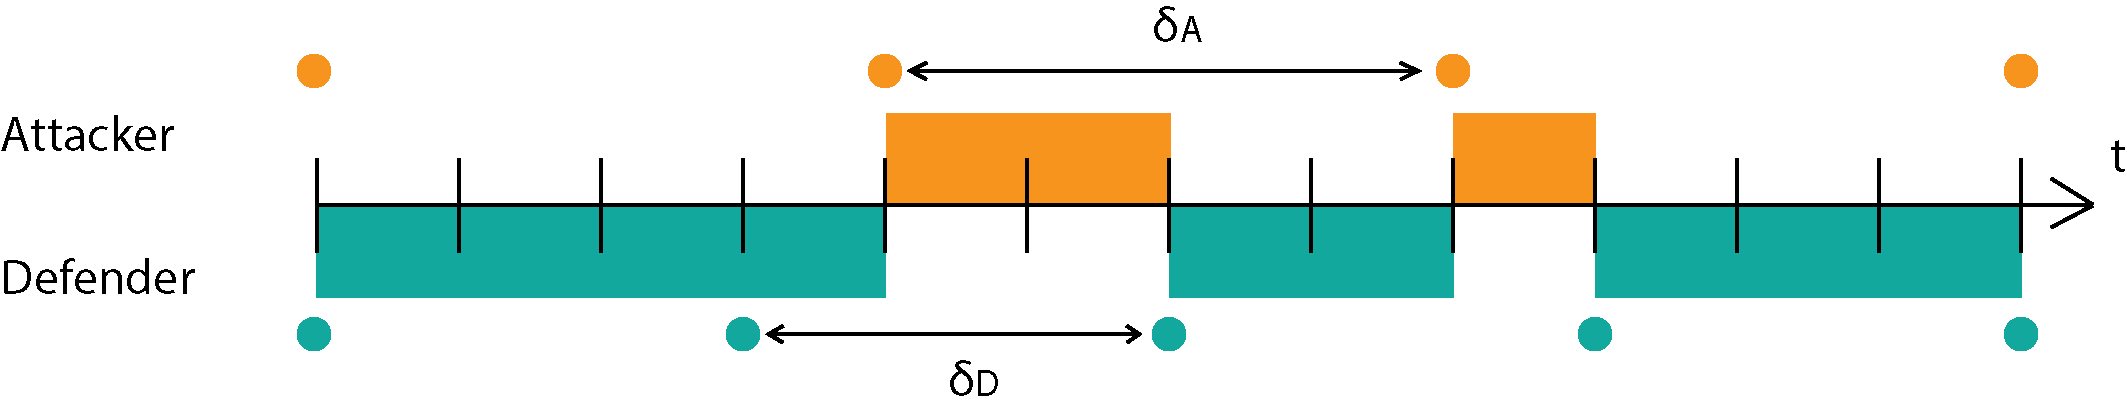
\includegraphics[scale=0.7]{../../doc/template/Images/FLipi.png}
\caption{A representation of a FlipIt game where both players are playing periodically. Every move or flip is indicated by a blue or orange circle. The attacker is represented in orange and plays with a period of $\delta_{A}=4$. The defender is represented in blue and plays with a period of $\delta_{D}=3$. The blue and orange rectangles represent the amount of time the respective player is in control of the resource.}
\label{fig:FLipItDefault}
\end{figure}



We denote the state of the resource as a time-dependent variable $C=C_{i}(t)$. 
$C_{D}(t)$ is 1 if the game is under control by the defender and 0 if the game is under control by the attacker. Reversely, $C_{A}(t)$ is 1 if the game is under control by the attacker and 0 if under control by the defender. So, $C_{A}(t)= 1 - C_{D}(t)$.
The game starts with the defender being in control: $C_{D}(0)= 1$. \\


The players receive a benefit equal to the time units they were in possession of the resource minus the cost of making their moves. The cost of a player \textit{i} is denoted by $k_{i}$. 
The total gain of player \textit{i} is equal to the total amount of time that a player \textit{i} has owned the resource from the beginning of the game up to time \textit{t}. It is expressed as follows:
\begin{equation}\label{first}
G_{i}(t) = \int_0^t \! C_{i}(x) dx.
\end{equation}
If we add up the gain of the defender and the gain of the attacker it should sum up to \textit{t}:
\begin{equation}\label{first}
G_{D}(t) + G_{A}(t) = t
\end{equation}
The average gain rate of player \textit{i} is defined as:
\begin{equation}\label{first}
\gamma_{i}(t) = G_{i}(t)/t.
\end{equation}
And thus for all $t > 0$ :
\begin{equation}\label{first}
\gamma_{D}(t) + \gamma_{A}(t) = 1
\end{equation}
Let $\beta_{i}(t)$ denote player's \textit{i} average benefit upto time \textit{t}:
\begin{equation}\label{first}
\beta_{i}(t) = \gamma_{i}(t) - k_{i}\alpha_{i}.
\end{equation}
This is equal to the fraction of time the resource has been owned by player \textit{i}, minus the cost of making the moves. ~$ \alpha_{i}$ defines the average move rate by player \textit{i} up to time \textit{t}.
In a given game, the asymptotic benefit rate (or simply benefit) will be defined as the lim inf of the average benefit because time\textit{ t} will increase to infinity and the average benefit may not have limiting values.
\begin{equation}
\beta_{i}(t)  = \lim_{t \to \infty} inf \beta_{i}(t) 
\end{equation}
\\


\subsubsection{strategies}
Because the players move in a stealthy way, there are different types of feedback that a player can get while moving. These types of feedback can be divided into two groups of strategies. The non-adaptive strategies and the adaptive strategies. These are described in table \ref{table:Strategies}. \\

If there is no feedback for either player, we have a non-adaptive strategy. Because a player does not receive any feedback during the game he will play in the same manner against every opponent. The strategy is called non-adaptive because the playing strategy is not dependent on the opponents movements. An interesting subclass of the non-adaptive strategies is the one where the time intervals between two consecutive moves are generated by a renewal process. An example of such renewal strategy is the periodic strategy where the time between two consecutive moves of the players are a fixed interval. An exponential strategy is a renewal strategy in which the interval between two consecutive moves is exponentially distributed. \\
In case there is feedback, a player can adapt his strategy to the information received about the opponent's moves. Depending on the amount of information received, two subclasses of adaptive strategies can be identified. The Last Move (LM) strategies represent the class where whenever a player flips he will find out the exact time that the opponent played the last time. In the second class, called Full History (FH), whenever a player flips he will find out the whole history of the opponent's move. \\
In this paper we restrict ourselves to periodic strategies. This choice is motivated by the fact that in a security game a player (defender or attacker) rarely has information about the moves (last move or full history) of his opponent.  \\


 \begin{table}
 \centering
 \begin{tabular}{ l | c  }
  \textbf{Categories} & \textbf{Classes of Strategies} \\
  \hline Non-adaptive (NA) & Renewal \\
  & - Periodic \\
  & ~~~ - Exponential \\
  & General non-adaptive \\
  \hline Adaptive (AD) & Last move (LM) \\
  & Full History (FH) \\  
\end{tabular}
 \caption{Hierarchy of Classes of strategies in FlipIt}
 \label{table:Strategies}
 \end{table}

\subsubsection{Results of the FlipIt game}
The study of the different strategies by means of FlipIt framework allows to derive a number of interesting results:  
\begin{itemize}
\item periodic games dominate the other renewal strategies, meaning that it is always advantageous to play periodically against an opponent with a renewal strategy;
\item periodic games are disadvantageous against players following a Last Move adaptive strategy;
\item if the defender plays with a periodic rate that is fast enough he'll force the attacker to drop out;
\item any amount of feedback about the opponent received during the game, benefits to a player.
\end{itemize}
 
 
\section{Extensions on FlipIt}
\label{ch1:extendedWork}

Various possible ways to extend FlipIt have already been proposed. 
Laszka et al. made a lot of additions and extensions to the original game of FlipIt. For instance Laszka et al. extended the basic FlipIt game to multiple resources. The rationale is that for compromising a system in real life, more than just one resource needs to be taken over. An example is that gaining access to deeper layers of a system may require breaking several passwords. The model is called FlipThem \cite{FlipThem}. Laszka et al. also use two ways to flip the multiple resources: the AND and the OR control model. In the AND model the attacker only controls the system if he controls all the resources of the system, whereas in the OR model the attacker only needs to compromise one resource to be in control of the entire system. \\

Another addition of Laszka et al. to the game of FlipIt \cite{MitigationCovert} 
is extending the game to also consider non-targeted attacks by non-strategic players. In this game the defender tries to maintain control over the resource that is subjected to both targeted and non-targeted attacks. Non-targeted attacks can include phishing, while targeted attacks may include threats delivered through zero day attack vulnerabilities. \\
One of the last important additions from Laszka et al. \cite{MitigationNonTargeted} is to consider a game with targeted and non-targeted attacks where the moves made by the attacker do not succeed immediately. This is similar to this paper but it has still some major differences. First the moves by the attacker are still covert but the moves made by the defender are known to the attacker. This means that the attacker knows when the defender plays and can change its strategy depending on the moves of the defender. Our motivation for a defender with stealthy moves is that there is not always an intelligent individual that is behind an APT. Some APTs don't know if the computer is already been recovered. There purpose is to spread. Not to check if they have already infected. \todo{beter verwoorden}. The second difference is that even though both the targeted and non-targeted attacks do not succeed immediately, the delay is determined differently. For the targeted attack the time till it succeeds is given by an exponential distributed random variable with a known rate. The non-targeted attacks are modelled as a single attacker and the time till it succeeds is given by a Poisson process. In our paper the delay is given by one parameter, that can be the result of any virus propagation model. The third and last difference is that the paper of Laska has multiple attackers and they try to find the best strategy of the defender against both targeted and non-targeted attacks. The conclusion of this paper is that the optimal strategy for the defender is moving periodically. \\ 

FlipIt has also been applied to several cases in system security. Reseachers explored different applications of FlipIt for real-world problems, like password reset policies, VM refresh, cloud auditing and key rotation \cite{ApplyingFlipit}. \\
Other authors used the FlipIt game to apply it on a specific scenario. To be able to use the FlipIt game, modifications where required for the FlipIt model.
One of the scenarios by Pham \cite{compromised} was to find out whether a resource was compromised or not by the attacker. This could be verified by the defender, who has an extra move "test" beside the flip move. The basic idea is to test with an extra action if the resource has been compromised or not. This move involves also an extra cost.\\
A three-player game has also been investigated where the flipit framework of two players is extended by another player. This player represents an insider that trades value information with the attacker \cite{fengstealthy}.\\


Finally researchers also have investigated the behaviour of humans playing FlipIt. A. Nochenson and Grossklags \cite{nochenson2013behavioral}  investigate how people really act when given temporal decisions. They found out that the results improves over time but that they are dependent on gender, age, and other individual difference variables. The result also shows that the participants perform generally better when they have more information about the strategy of the opponent which is a computerized player. Reitter et al. \cite{reitter2013risk} extended the work of A. Nochenson and Grossklags to include various visual presentation modalities for the available feedback during the investigation.\\




% --------------- example of a game -----------------%


%------------------------------------------------%
%            Intro about virusses				 %
%------------------------------------------------%


\chapter{FlipIt game with virus propagation}
\label{chapter2:FlipIt with virus propagation}
%\documentclass[10pt]{article}
%\begin{document}

%%%%%%%%%%%%%%%%%%%%%%%%%%%%%%%%%%%%%%%%%%%%%%%%%%%%%%%%%%
%%%%%			Introduction Chapter 1				%%%%%%
%%%%%												%%%%%%
%%%%%												%%%%%%
%%%%%%%%%%%%%%%%%%%%%%%%%%%%%%%%%%%%%%%%%%%%%%%%%%%%%%%%%%

\section{Introduction}
\label{Ch2:Intro}
The game of FlipIt with virus propagation considers attackers where their moves are not instantaneous. This can be motivated by an example of a virus. A virus can be dropped on a network but it only compromises the whole network if every node in the network is infected. The basic FlipIt game does not take this into account. In this chapter the FlipIt game with virus propagation is explained and how it can be modelled. First the main differences with the basic FlipIt game are discussed in section \ref{ch2:diffFlip}. Next in section \ref{ch2:formal} the formal definition of the game with virus propagation is given. At last, in section \ref{ch2:periodicvirus} a periodic strategy game is considered and the formalization of the formulas with virus propagation are determined.\\

This chapter explains how to model a FlipIt game with a virus propagation that infects a network. The first section explains the difference between a normal FlipIt game and a FlipIt game with virus propagation. The next section derives a formula to calculate the benefit for a FlipIt game with a virus propagation. In the last section we calculate the Nash equilibrium for the benefit formula.
\section{FlipIt game with virus propagation}

Welke aanpassing en motivatie: attacker 1 speler die elke keer virus probeert te droppen. Defender die elke keer patcht als er virus gedropt wordt. Elke patch voldoet aan de meest recente patch dus alle virussen die ook gedropt zijn worden weggedaan. Voor future work: patch systeem aanpassen. 

The actions of a defender: the actions of an attacker:

\section{Explaining difference between FlipIt with and without virus propagation}
\label{ch2:diffFlip}
\begin{figure}[hbtp]
\caption{The first game is the basic FlipIt game. The second is a FlipIt game with a delay. During the first flip of the attacker, the defender moves after the delay, causing the attacker to get control over the resource. During the second flip of the attacker, the defender flips at time t+d, causing the defender to take control over the resource before the attacker. During the third and final flip of the attacker, the defender flips during time t+d, causing the attacker to never gain control over the resource. }
\centering
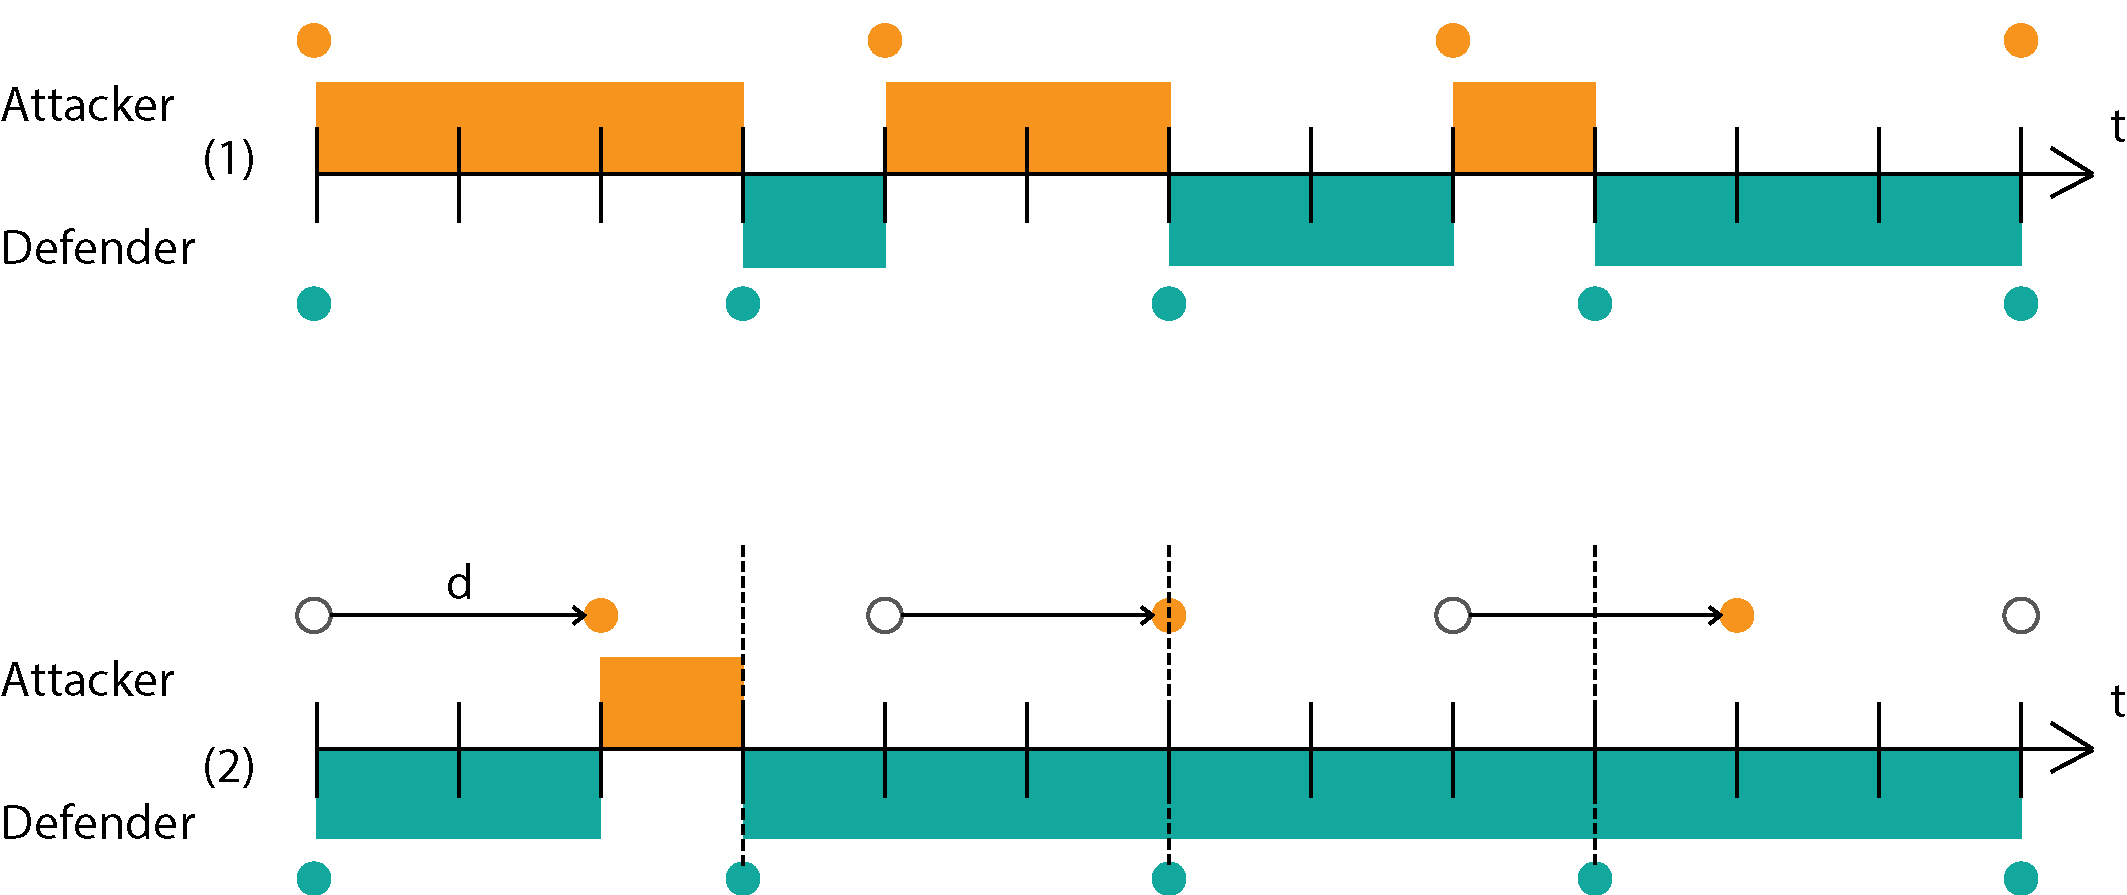
\includegraphics[scale=0.7]{Images/dtFlip.png}
\label{dt}
\end{figure}

A FlipIt game consists of a single resource. To represent the security problem, the game now defines its single resource as a computer network with multiple
nodes. One of the players, the defender, will try to defend his network. The defender
will do this by flipping all the nodes of the network (i.e. the entire resource) in every move he plays. The
attacker on the other hand will try to infect all the nodes in the network. The attacker
will do this by flipping the node in the graph that can infect all the nodes in the
shortest possible time. After dropping a virus on the first node, it takes a while for the virus to infect the entire network. Since the original FlipIt game works with a single resource that is always flipped entirely, the assumption is made that the attacker is considered to gain immediate full control over the resource when the network has been infected, even it is only one node that has been infected.\\

In reality however, after dropping a virus on the first node, it takes a while for the virus to infect
the entire network. So, the assumption that the attacker has full control over the resource as soon as a node has been infected, is not realistic. The attacker has only control of the network once all or a sufficient number of nodes are infected. 
The time that it takes for the virus to infect every node (or a sufficient number of nodes) will be
denoted as an infection-delay variable \textit{d} (called 'delay' for short in the remainder of this paper). If we want to measure how long it takes for the virus to
infect all the nodes in the network, we have to calculate the shortest path from the
first infected node to the farthest node. Rather than denoting the time needed for infecting \textit{all} the nodes, the variable $d$ can also be used to denote the time needed to infect \textit{a sufficient number} of nodes.

Assume that an attacker attacks at time \textit{t}, he doesn't get immediate control over the resource, but he only gains control at time \textit{t + d}, with $d$ denoting the time needed to infect a sufficiently number (or all) nodes. If the defender flips the network before the period $d$ has elapsed (so, somewhere between $t$ and $t + d$), then the attacker will never gain full control over the resource. See figure \ref{dt}. This implies that the mathematical formulas for gain and benefit need to be adapted to the fact that the attacker loses part of its benefit because of this delay. In the remainder of this paper, we will adapt the formalization of the FlipIt game using the variable $d$. \\ 


%%------------------------------------------------%
%%            Intro Game Theory 					 %
%%------------------------------------------------%
%\subsection{Actions of the attacker}
%A virus has different kind of ways of making his way through a company network. We will describe the different ways of how the virus can propagate. For start we will say that the virus or worm will be dropped on Node i and that it has k numbers of neighbours. 
%\begin{enumerate}
%\item Node i is infected and will spread the virus or worm to every k neighbours and will stop infecting the neighbours in the next step
%\item Node i is infected and will spread the virus or worm to every k neighbours and will keep on spreading the virus to the same neighbours in every next step
%\item Node i is infected and will spread the virus to only one of the k neighbours and will stop infecting another neighbour in the next step
%\item Node i is infected and will spread the virus to only one of the k neighbours and in the next step it will infect another one of the k neighbours 
%\end{enumerate}
%
%In the game that will be modelled in the paper we will use the settings of the first spreading method. We will not use method 2 because this kind of propagation will float the network. Because we use the settings of a mail system and contact in a mailing list the method of 3 and 4 are not used. \\
%In the first method the node that has been infected can be again infected. If one of the neighbours infects the node again the node will infect his neighbours again. By using this spreading method we have three distinct states in which a node can be situated. An \textit{infected state}, a \textit{clean state} and a \textit{spreading state}. An infected state means that the node is infected and will not spread the virus to its neighbours, a clean state means that the node is not infected on that moment and a spreading state means that the node is infected and that it will spread the virus or worm to its neighbours in the next step.
%We can argument this kind of propagation through a mail worm. \todo{voorbeeld geven van zo een worm}
%%Another propagation method is that the virus works as a token. It will propagate to only one neighbour and continue to spread. 
%
%The Attacker itself has two different ways of attacking the company network. It will only infected one node of the network and will wait for the virus to spread itself through the network. We will model two ways of attacks of an Attacker:
%\begin{enumerate}
%\item The attacker drops the virus on a random node on the network
%\item The attacker drops the virus on a targeted node on the network
%\end{enumerate}
%The attacker in this game will put a virus or worm on one of the nodes in the network. (This will happen at random.) The attacker does not know on which node the virus will be dropped. We will use this randomness because \todo{feit uit security rapport symantec} most viruses are spread via a usb stick or a shared resource. If we use this spreading method where we have a targeted attack the attacker will have more information about the network. \\
%
%The attacker can choose at which rate it will drop a virus on one of the nodes on the network. The cost of dropping a virus will be the same. It will not increase. If it will increase this means that the attacker will eventually drop out of the game because it becomes to expensive.\\
%The attacker is in control over the game if it manages to infect a subset of all the resources of the company network.
%
%
%\subsection{Actions of the defender}
%The attacker wants to protect all the nodes of his network. It can do so by getting back control over the resources. We will assume that the defender of the network has knowledge over his own network. Which is convenient in the real world because a company has to know how his infrastructure looks like.\\
%
%The defender has two possible ways of defending its network:
%\begin{enumerate}
%\item The defender flips all the nodes of his network
%\item The defender will flip a subset of the nodes of his network
%\end{enumerate}
%
%The cost of flipping all the nods of the network will be greater than the cost of flipping a subset of nodes. We make this assumption because otherwise it will be beneficial for the defender to always flip all the nodes in the network.\\
%
%We will also make the assumption that as a defender flips a node the node can get infected again. A flip will not be  correlated to a patch but to a clean-up. \todo{waarom geen patch, wormen kunnen veranderen gaandeweg}
%\todo{andere mogelijkheid:} Another setting of the game can be that the flip of the defender is equal to a patch and that the resource cannot be infected any more. But with this case we deviate from the flipIt game, because the attacker cannot flip the resource any more. Unless we work with different virusses every time the attacker flips. We start with the less complex game of flipping is equal to a clean-up.




\section{Playing periodically with virus propagation}
\label{ch2:periodicvirus}




The formalization starts from the model of the non-adaptive continuous basic FlipIt game where players use a periodic strategy with a random phase. This choice is motivated by the assumption that in most organisations, the defence strategy is to periodically defend the network. This corresponds to a periodic defender strategy.  A periodic attacker strategy is assumed as well, to be able to compare the results with the periodic strategy of the FlipIt game in \cite{FlipIt}. %, as this also corresponds to a common real life strategy. %nog eventueel verder te motiveren
Further research can investigate the effect of relaxing this assumption. \\



Similarly as in \cite{FlipIt}, we split the formalization in two cases. The first case is where the defender plays at least as fast as the attacker, the second case is where the attacker plays at least as fast as the defender. For each of these cases, first the benefit formula of the basic case without delay is presented, and then the delay is introduced.  \\

Intuitively we could assume that $d$ can never be bigger than $\delta_{A}$ because then the benefit for the defender would always be 1. This is not always true. It is only true if $d$ is bigger than $\delta_{D}$, because then the defender will always be in control. For this we only calculate the formulas for the cases where $d$ is smaller than $\delta_{D}$. We can already conclude that it is no use for the attacker to play when the delay is bigger than $\delta_{D}$. \\

\subsection{Formalization the benefit formula including the infection-delay}



 A Periodic strategy is a non-adaptive renewal strategy where the time intervals between consecutive moves are a fixed period, denoted by $\delta$. Moreover it has a random phase, that is chosen uniformly and random in the interval $[0,\delta]$ for the first move. The average rate of play of a player is denoted by $\alpha_{i} = \dfrac{1}{\delta_{i}}$. List of symbols that will be used throughout the paper. Figure \ref{FlipItDelay} represents a couple of the symbols for clarification.\\
~~\\
\begin{figure}[hbtp]
\caption{Formalization of a FlipIt game with delay: A representation of a FlipIt game where both players are playing periodically. Every move or flip is indicated by a blue or orange circle.  The defender is represented in blue and plays with a period of $\delta_{D}$. The flip of the attacker is represented by a white circle, but because there is a delay d, the attacker only controls the resource after time d represented by an orange circle. The attacker plays with a period of $\delta_{A}$. The blue and orange rectangles represent the amount of time the respective player is in control of the resource.}
\centering
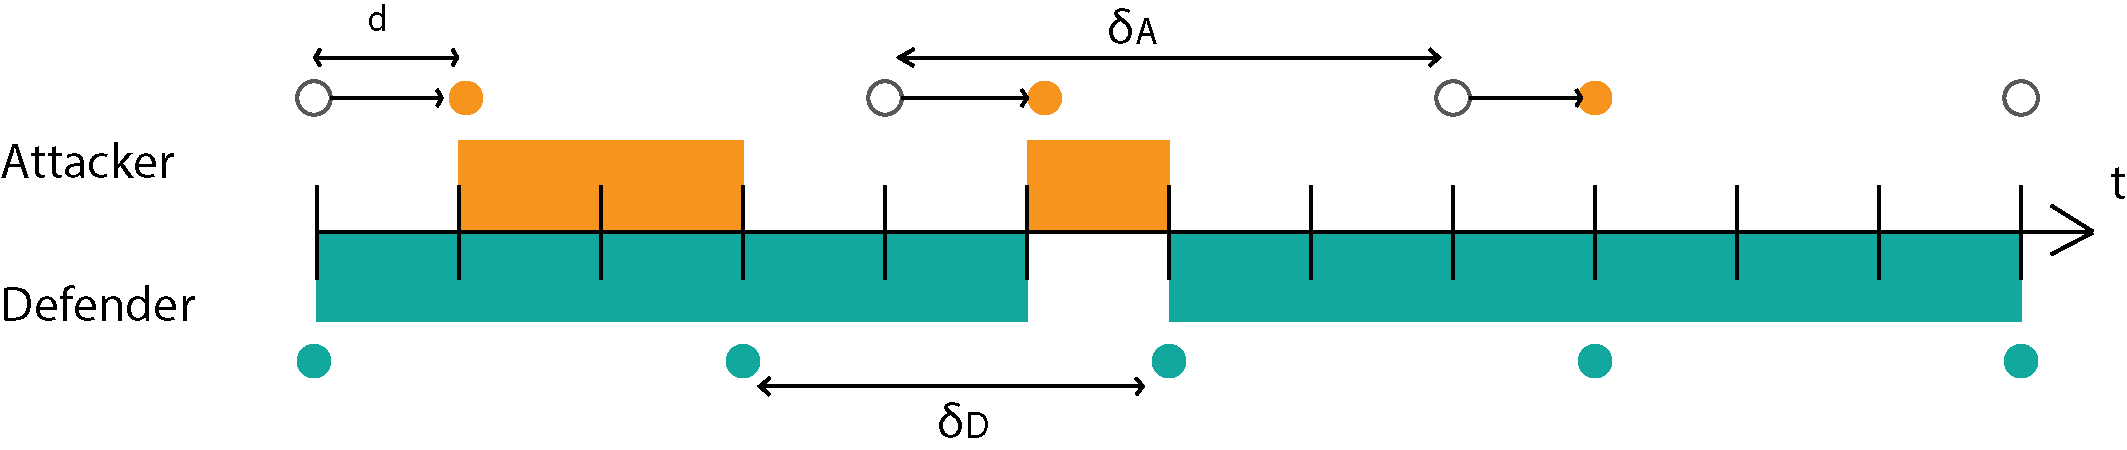
\includegraphics[scale=0.7]{Images/DefFlip.png}
\label{FlipItDelay}
\end{figure}

\begin{description}
\item $i$: Defines the player. Different as in the FlipIt paper where the defender is denoted by the subscript 0 and the attacker by the subscript 1.
\item $\delta_{i}$: The length of the interval between two consecutive moves of player \textit{i}. 
\item $\alpha_{i}$: The average flip rate of player \textit{i}, given by $\alpha_{i}=1/\delta_{i}$.
\item $k_{i}$: The cost of player \textit{i}'s moves.
\item $d$: The delay caused by the virus propagation.
\item $G_{i}(t)$: The total gain of player \textit{i} denotes the amount of time player \textit{i} is in control over the resource up to time \textit{t}.
\item $\gamma_{i}$: The average gain rate of player \textit{i} defined as $G_{i}(t)/t$
\item $\beta_{i}$:  The average benefit rate up to time \textit{t} defined as  $\beta_{i} = \gamma_{i} -k_{i} \alpha_{i} $.
\item $opt_{i}$: The optimum function.
\end{description}




\subsection*{\textbf{Case 1:} $\delta_{D} \leq \delta_{A} $ (The defender plays at least as fast as the attacker.) }

Let $r = \dfrac{\delta_{D}}{ \delta_{A} }$. The intervals between two consecutive defender's moves have length $\delta_{D}$. Consider a given defender move interval. The probability over the attacker's phase selection that the attacker moves in this interval is r. Given that the attacker moves within the interval, he moves exactly once within the interval (since $\delta_{D} \leq \delta_{A} $) and his move is distributed uniformly at random. \\

The expected period of attacker control within the interval would be r/2, without considering the delay by a virus. Therefore the benefit for the attacker, without considering the delay, can be expressed as follows:

\begin{equation*}
\beta_{A}(\alpha_{D},\alpha_{A}) =\dfrac {r} {2} - k_{A} \alpha_{A} = \dfrac {\delta_{D}} {2\delta_{A}} - k_{A} \alpha_{A}  
\end{equation*}\\

Correspondingly, the benefit for the defender can be expressed as:
\begin{equation*}
\beta_{D}(\alpha_{D},\alpha_{A}) =1 -  \dfrac {r} {2} - k_{D} \alpha_{D} = 1 - \dfrac {\delta_{D}} {2\delta_{A}} - k_{D} \alpha_{D} 
\end{equation*}

\begin{figure}[hbtp]
\caption{Case 1: Difference between a basic FlipIt game and a FlipIt game with a delay. (1) is the FlipIt game without a delay and (2) is with a delay. The delay is denoted with an arrow. The attacker is only in control when the circle becomes orange.}
\centering
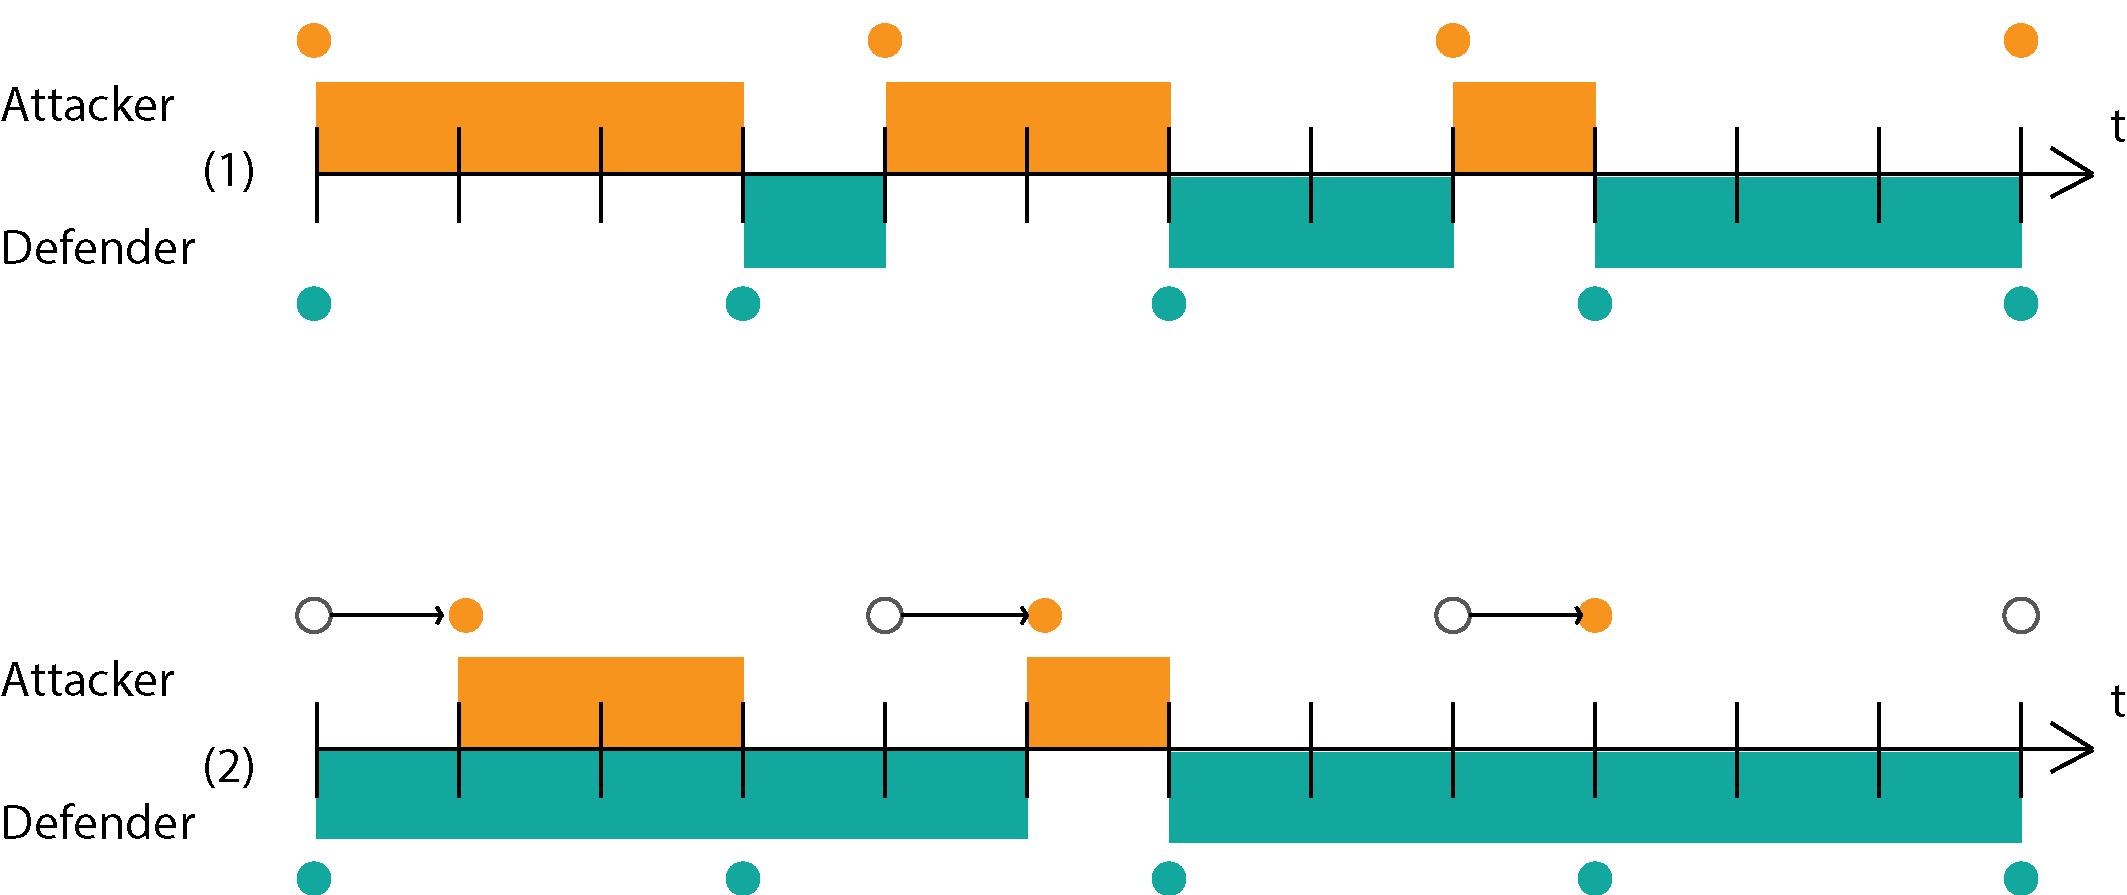
\includegraphics[scale=0.6]{../../doc/template/Images/DiffDelayCase1.png}
\label{fig:delaycase1}
\end{figure}


However, because of the delay required for virus propagation, the maximal time of control is reduced to $\delta_{D}-d$ , see figure \ref{fig:delaycase1}. There is a probability of \textit{r} that the attacker will move in the interval of the defender. However, the gain will not be half of the interval. Indeed, the attacker has to play soon enough to gain control, meaning that the attacker has to play during the period of $\delta_{D}-d$ during the interval of the defender. The probability that the attacker plays soon enough is $\dfrac{\delta_{D}-d}{\delta_{D}}$ and this will give the attacker an average gain of $\dfrac{\delta_{D}-d}{2}$. If the attacker moves after the period of $\delta_{D}-d$, the gain of the attacker will be zero. The probability that this happens is  $\dfrac{d}{\delta_{D}}$. The average gain rate of the attacker can then be expressed as follows if we look at one interval of the defender:
\begin{equation*}
\gamma_{A}(\alpha_{D},\alpha_{A}) = \dfrac {1}{\delta_{D}} [ \dfrac{\delta_{D}}{\delta_{A}} \cdot \dfrac{\delta_{D}-d}{\delta_{D}} \cdot \dfrac{\delta_{D}-d}{2} + \dfrac{\delta_{D}}{\delta_{A}} \cdot \dfrac{d}{\delta_{D}} \cdot 0 ]
\end{equation*}

To derive the benefit, the cost of moving is subtracted from the average gain. 
\begin{equation*}
\beta_{A}(\alpha_{D},\alpha_{A}) = \dfrac { (\delta_{D}-d) ^{2}} {2 \cdot \delta_{D}  \delta_{A}} - k_{A} \alpha_{A}
\end{equation*}
\begin{equation*}
\beta_{A}(\alpha_{D},\alpha_{A}) = \dfrac { \delta_{D}} {2 \cdot \delta_{A}} - k_{A} \alpha_{A} - ( \dfrac{d^{2}}{2 \cdot \delta_{A} \delta_{D}} - \dfrac{d}{\delta_{A}} )
\end{equation*}
 
 
 The benefit of the defender is expressed as follows:
\begin{equation*}
\beta_{D}(\alpha_{D},\alpha_{A}) = 1 - \dfrac { (\delta_{D}-d) ^{2}} {2 \cdot \delta_{D}  \delta_{A}} - k_{D} \alpha_{D}
\end{equation*}
~~\\
We can easily see that when $d$=0, we obtain the formula of the original FlipIt game.\\





\subsection*{\textbf{Case 2:} $\delta_{A} \leq \delta_{D} $ (The attacker plays at least as fast as the defender.) }

First let $r = \dfrac{\delta_{D}}{ \delta_{A} }$. The intervals between two consecutive attacker's moves have length $\delta_{A}$. Consider a given attackers move interval. The probability over the attacker's phase selection that the defender moves in this interval is $\dfrac{\delta_{A}}{ \delta_{D} } = (1/r)$. Given that the defender moves within the interval of the attacker, he moves exactly once within this interval (since $\delta_{A} \leq \delta_{D} $) and his move is distributed uniformly at random. \\

A similar analysis as in case 1 for a FlipIt game without virus propagation yields the following benefits:

\begin{equation*}
\beta_{D}(\alpha_{D},\alpha_{A}) = \dfrac {1} {2r} - k_{D} \alpha_{D} = \dfrac {\delta_{A}} {2\delta_{D}} - k_{D} \alpha_{D} 
\end{equation*}
\begin{equation*}
\beta_{A}(\alpha_{D},\alpha_{A}) =1 - \dfrac {1} {2r} - k_{A} \alpha_{A} = 1- \dfrac {\delta_{A}} {2\delta_{D}} - k_{A} \alpha_{A}  
\end{equation*}\\

An intuitive solution for the case with a virus would be to subtract the benefit of the attacker received in each interval with the delay similarly as in case 1. This would give us the following formula if we derive it in the same way:
\begin{equation*}
\beta_{A}=\dfrac{(\delta_{A} - d)^2}{2\delta_{A}\delta_{D}} - \dfrac{k_{A}}{\delta_{A}}
\end{equation*}

But this results in an overestimation. How closer $\delta_{A}/\delta_{D}$ is equal to one, the better the approximation. If $\delta_{A}/\delta_{D} = 1$ the result is correct. This formula does not take into account that if the attacker was in control in the previous interval, the delay should not be subtracted, because the delay will not be in control of the defender. This means that we have to look at what happens in the previous interval. \\

From the defender we know that his moves are instantaneous. It is easier to calculate the benefit of the defender in this case. Because the defender moves slower than the attacker we know that if the defender moves during the interval of the attacker, he only moves once within this interval.
The defender will move during the interval of the attacker with a probability of $\dfrac{\delta_{A}}{\delta_{D}} $. When this happens the defender will end with being in control at the end of the interval. In the next interval the attacker will have to regain control, meaning that during the delay, the defender stays in control, see figure \ref{fig:case2} cases (1) and (2). The defender will keep the control over the resource in the next interval over a period of the delay, namely \textit{d}. \\

Consider a timespan $\delta_{A} + d$, representing the attacker's interval followed by the delay period in his next interval. The defender will never move twice during this timespan because $\delta_{A} + d \leq \delta_{D}$.
Because $d + \delta_{A} \leq \delta_{D}$ the next move of the defender in this second interval will never occur during the delay, meaning that the entire delay can be considered as an extra benefit resulting of a play in the previous interval. 
So, every time the defender plays, he will get an average gain of $\dfrac{\delta_{A}}{2}$ in the interval where he plays and in the next interval will always receive a extra gain of $d$, yielding a total average gain per interval of
$\dfrac{(d+\dfrac{\delta_{A}}{2})}{\delta_{A}}$

For the case with a virus we consider two cases, Case a and Case b, depending on whether the delay is shorter or longer than the difference between the attacker's and the defender's period.  \\


\subsubsection*{\textbf{Case a:} $d + \delta_{A} \leq \delta_{D}$}

The total gain  rate of the defender is then the probability that the defender will move during an interval of the attacker multiplied by the total average gain per interval: 

\begin{equation*}\label{first}
\gamma_{D}(\alpha_{D},\alpha_{A}) = \dfrac{\delta_{A}}{\delta_{D}} \cdot \dfrac{(d+\dfrac{\delta_{A}}{2})}{\delta_{A}} 
\end{equation*}
\begin{equation*}\label{first}
\gamma_{D}(\alpha_{D},\alpha_{A}) = \dfrac{\delta_{A}}{2\delta_{D}} + \dfrac{d}{\delta_{D}} 
\end{equation*}\\
This yields in the following benefit formula:
\begin{equation*}\label{first}
\beta_{D}(\alpha_{D},\alpha_{A}) = \dfrac{\delta_{A}}{2\delta_{D}} + \dfrac{d}{\delta_{D}} - k_{D} \alpha_{D} 
\end{equation*}\\

The benefit for the attacker will be as follows:
\begin{equation*}\label{first}
\beta_{A}(\alpha_{D},\alpha_{A}) = 1 -\dfrac{\delta_{A}}{2\delta_{D}} - \dfrac{d}{\delta_{D}} - k_{A} \alpha_{A} 
\end{equation*}\\

\begin{figure}[hbtp]
\caption{All possible cases for the attacker and the defender in Case 2.A where $d + delta_{A} < delta_{D}$. As can be seen, the defender will have control during a period of \textit{d} over the resource when the defender has flipped in the previous interval.}
\centering
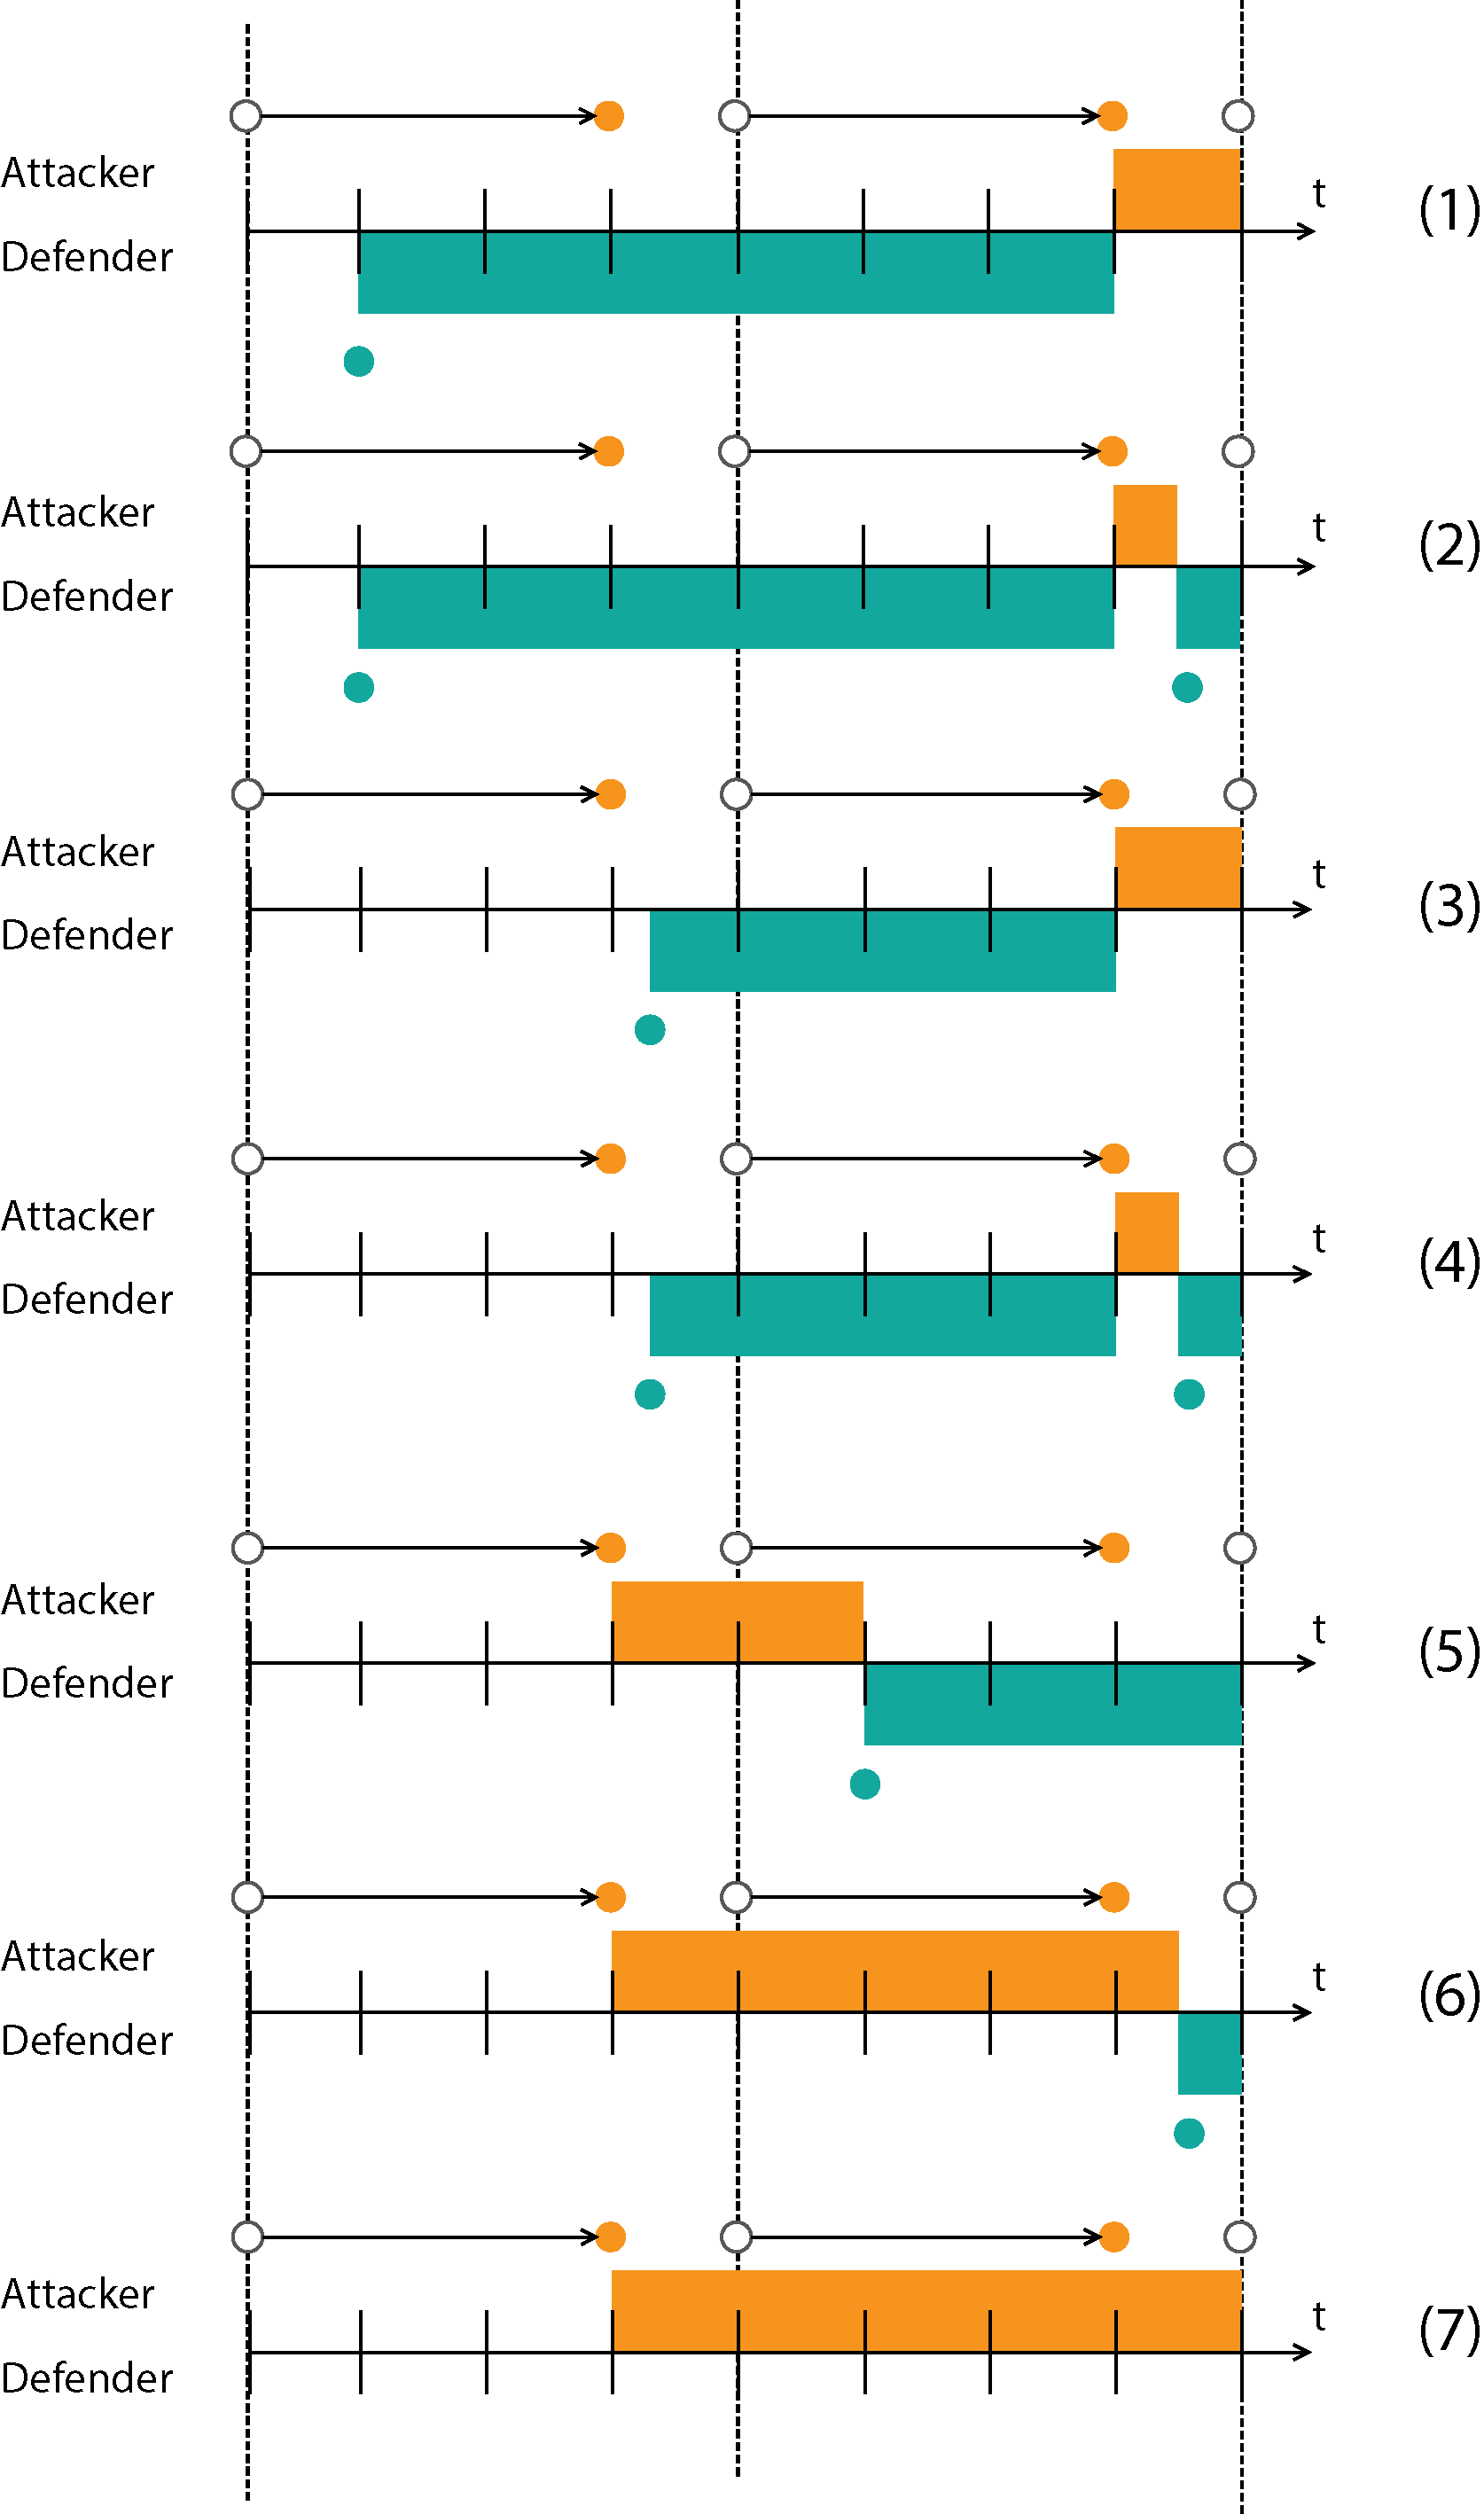
\includegraphics[scale=0.7]{../../doc/template/Images/FlipItCase2a.png}
\label{fig:case2}
\end{figure}


It is crucial that $ \delta_{D}$ is at least as large as $d + \delta_{A}$. If not, this would mean that the defender can move during the delay in the interval following the interval where the defender already moved. This would mean that there can be an overlap between the average gain of $\dfrac{\delta_{A}}{2}$ and the delay. The above benefit formula would then include to much gain for the defender: the potential overlap during the delay would be counted twice. \\


~~ \\
\subsubsection*{\textbf{Case b:} $d + \delta_{A} \geq \delta_{D}$}
~~~\\

To obtain the formula in case of a too long delay, we therefore need to subtract this overlapping gain from the above formula. 
Since $\delta_{D} \geq \delta_{A}$, if the defender enters the interval immediately after the attacker has played, then the defender cannot have played in the previous interval. In that case, there is no overlap. So the problem of the overlap only appears if the defenders enters late enough and thus only the last part of the delay is subject to overlap. The larger the difference between the interval of the defender and the attacker, the smaller the risk of overlap. Concretely, only the last part of length $d - (\delta_{D} - \delta_{A})$ is subject to overlap. Hence, the probability of overlap is $\dfrac{ d - (\delta_{D} - \delta_{A})}{\delta_{D}}$ and the gain will be half of this interval:  $\dfrac{ d - (\delta_{D} - \delta_{A})}{2}$.  The gain rate to be subtracted is therefore:\\

\begin{equation*}
\dfrac{1} {\delta_{A}} \cdot \dfrac{d - (\delta_{D} - \delta_{A})}{\delta_{D}} \cdot \dfrac{d - (\delta_{D} - \delta_{A})}{\delta_{D}}
\end{equation*}

The total gain  rate of the defender is obtained by subtracting this term from the gain rate of case a:
 \begin{equation*}
\gamma_{D}(\alpha_{D},\alpha_{A}) = \dfrac{\delta_{A}}{\delta_{D}} \cdot \dfrac{(d+\dfrac{\delta_{A}}{2})}{\delta_{A}} - \dfrac{(d - (\delta_{D} - \delta_{A}))^{2}}{2 \delta_{D} \delta_{A}}
\end{equation*}
\begin{equation*}
\gamma_{D}(\alpha_{D},\alpha_{A}) = \dfrac{\delta_{A}}{2\delta_{D}} + \dfrac{d}{\delta_{D}} - \dfrac{(d - (\delta_{D} - \delta_{A}))^{2}}{2 \delta_{D} \delta_{A}}
\end{equation*}\\
This yields in the following benefit formula:
\begin{equation*}
\beta_{D}(\alpha_{D},\alpha_{A}) = \dfrac{\delta_{A}}{2\delta_{D}} + \dfrac{d}{\delta_{D}} - k_{D} \alpha_{D} - \dfrac{(d - (\delta_{D} - \delta_{A}))^{2}}{2 \delta_{D} \delta_{A}}
\end{equation*}\\
 
The benefit for the attacker will be as follows:
\begin{equation*}
\beta_{A}(\alpha_{D},\alpha_{A}) = 1 -\dfrac{\delta_{A}}{2\delta_{D}} - \dfrac{d}{\delta_{D}} - k_{A} \alpha_{A} + \dfrac{(d - (\delta_{D} - \delta_{A}))^{2}}{2 \delta_{D} \delta_{A}}
\end{equation*}\\






\chapter{Nash Equilibria}
\label{chapter:Nash}
%\documentclass[10pt]{article}
%\begin{document}

%%%%%%%%%%%%%%%%%%%%%%%%%%%%%%%%%%%%%%%%%%%%%%%%%%%%%%%%%%
%%%%%			Introduction Chapter 1				%%%%%%
%%%%%												%%%%%%
%%%%%												%%%%%%
%%%%%%%%%%%%%%%%%%%%%%%%%%%%%%%%%%%%%%%%%%%%%%%%%%%%%%%%%%

\section{Nash Equilibria}
%TODO-- rechtstreeks uit FlipIt paper --\\

In this chapter we are interested in finding the optimal strategies. To calculate the optimal strategies of both players we have to find the Nash Equilibria of the game. First the optimal functions are derived from the formulas in the previous chapter. From these piecewise functions we can derive the Nash Equilibria. \\

Nash equilibria are points with the property that neither player benefits by deviating in isolation from the equilibrium. We can compute Nash Equilibria for the periodic game as an intersection point of curves $opt_{D}$ and $opt_{A}$. 
\\
%As a second step, we are interested in finding Nash equilibria, points
%for which neither player will increase his benefit by changing his rate of play. 
More formally, a Nash equilibrium for the periodic game is a point $(\delta_{D}^{*},\delta_{A}^{*})$ such that
the defender's benefit $\beta_{D}(\alpha_{D},\delta_{A}^{*}) $is maximized at $\delta_{D}= \delta_{D}^{*}$ and the attacker's benefit
$\beta_{A}(\delta_{D}^{*},\delta_{A}) $ is maximized at $\delta_{A}= \delta_{A}^{*}$.
To begin with, some useful notation. We denote by $opt_{D}(\delta_{A}$) the set of values (rates
of play $\delta_{D}$) that optimize the benefit of the defender for a fixed rate of play $\delta_{A}$ of the
attacker. Similarly, we denote by $opt_{D}(\delta_{D}$) the set of values (rates of play $\delta_{A}$) that optimize
the benefit of the attacker for a fixed rate of play $\delta_{D}$ of the defender. \\

To determine $opt_{D}(\delta_{A})$ we need to compute the derivative of  $\beta_{D}(\delta_{D},\delta_{A}) $ for a fixed $\delta_{A}$.
 We consider two cases, where case 2 is divided into two subcategories. 
% Fig \todo{fig} shows all the cases.\\
%\begin{figure}[hbtp]
%\centering
%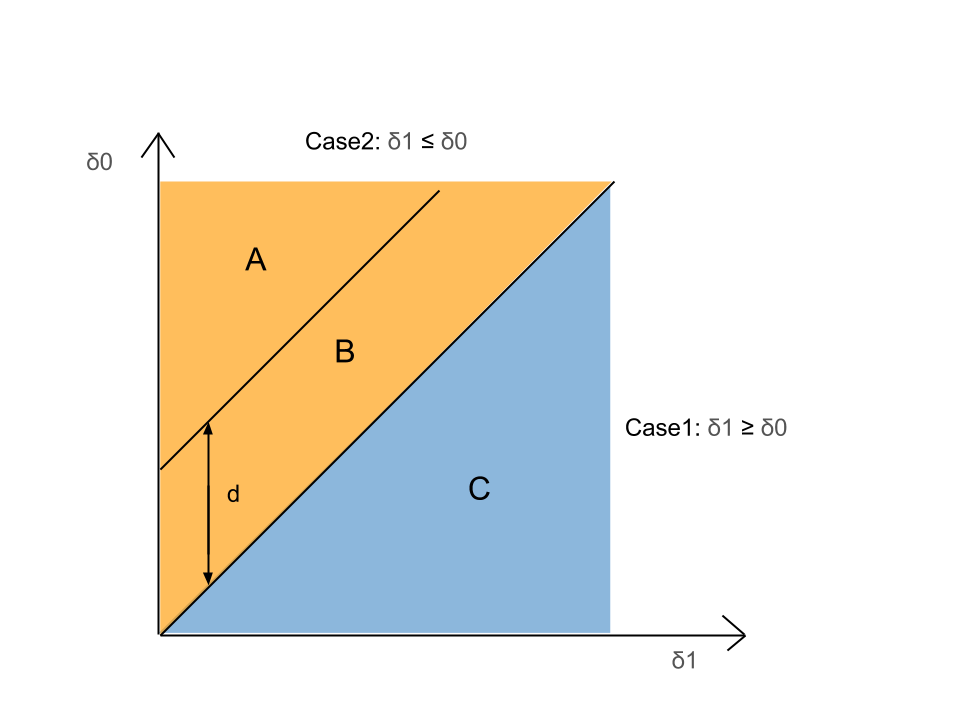
\includegraphics[scale=0.4]{Images/bestresp.png}
%\caption{This figure shows the all the cases with their subcategories. 'A' stands for Case 2.A: $\delta_{D} \geq d+\delta_{A} \geq \delta_{A}$ and 'B' stands for Case 2.B: $d+\delta_{A} \geq \delta_{D} \geq  \delta_{A} $ }
%\label{grafiekbestr}
%\end{figure}

\subsection{Determining the piecewise functions $opt_{D}(\delta_{A})$}


\subsection*{Case 1: $\delta_{D} \leq \delta_{A} $}
The benefit formula obtained in the previous chapter (formula \ref{Benfcase1:defender}) for the defender in this case is as follows:
\begin{equation*}
\beta_{D}(\delta_{D},\delta_{A}) = 1 - \dfrac{\delta_{D}}{2\delta_{A}} - \dfrac{d^{2}}{2\delta_{D}\delta_{A}} + \dfrac{d}{\delta_{A}}  - \dfrac{k_{D}}{\delta_{D}}
\end{equation*}

To know if the function decreases or increases we take the partial derivative of this formula for a fixed $\delta_{A}$:
\begin{equation*}\label{formdelta}
\frac{\partial \beta_{D}(\delta_{D},\delta_{A})}{\partial \delta_{D}} = - \dfrac{1}{2\delta_{A}} + \dfrac{k_{D}}{\delta_{D}^{2}} + \dfrac{d^{2}}{2\delta_{D}^{2}\delta_{A}}
\end{equation*}

The stationary points (maximum, minimum) can be found by setting the first derivative equal to zero and finding the roots of the resulting equation:
\begin{equation*}
\frac{\partial \beta_{D}(\delta_{D},\delta_{A})}{\partial \delta_{D}} =0 ~~~~~~ =>~~~~~~ \delta_{D} = \sqrt{2\delta_{A}k_{D} + d^{2}}
\end{equation*}

This leads to the following deduction given the sign of the coefficient of $\delta_{D}^{2}$: The function increases on $[0, \sqrt{2\delta_{A}k_{D} + d^{2}}]$ and is decreasing on $[\sqrt{2\delta_{A}k_{D} + d^{2}}, \infty]$. So we have a maximum at $\delta_{D} = min \{ \delta_{A}, \sqrt{2\delta_{A}k_{D} + d^{2}} \} $. Taking the minimum of the two values is needed because $\delta_{D}$ cannot be larger than $\delta_{A}$. \\
~~\\


\subsection*{Case 2.A: $\delta_{D} \geq d+\delta_{A} \geq \delta_{A} $ }

The benefit formula obtained in the previous chapter (formula \ref{benfcase2a:defender}) for the defender in this case is as follows:
\begin{equation*}
\beta_{D}(\delta_{D},\delta_{A})= \dfrac{\delta_{A}}{2\delta_{D}} + \dfrac{d}{\delta_{D}} - \dfrac{k_{D}}{\delta_{D}} = \dfrac{\delta_{A} + 2 (d-k_{D})}{2\delta_{D}}
\end{equation*}

Given that $\delta_{D}$ is always positive, the benefit function can be either increasing or decreasing depending on the numerator of the above fraction. \\

For $\delta_{A} + 2(d-k_{D}) > 0$ the benefit will be always positive but decreasing, see figure \ref{ShapeUp}. 
The defender will always play if $\delta_{A} + 2(d-k_{D}) > 0$ for $k_{D} < d$ or $k_{D} > d$ because $\delta_{A}$ will be positive in either case. There is an edge case if $d=k_{D}$, which results in a benefit of $\beta_{D}(\delta_{D},\delta_{A})= \dfrac{\delta_{A}}{\delta_{D}}$. \\
\begin{figure}
\centering
\includegraphics[scale=0.5]{Images/ShapesUp.png} 
\caption{The benefit function is of the shape of 1/x if $\delta_{D}$ is always decreasing and if $\delta_{A} + 2(d-k_{D}) > 0$. }
\label{ShapeUp}
\end{figure}

For $\delta_{A} + 2(d-k_{D}) < 0$, the benefit will always be negative so the defender will not play. See figure \ref{ShapeDown}. This is independent of the value of $k_{D}$ and $ d$. \\

\begin{figure}
\centering
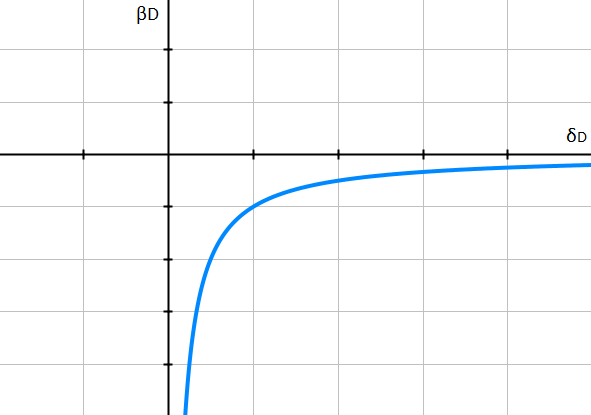
\includegraphics[scale=0.5]{Images/ShapeDown.png} 
\caption{The benefit function is of the shape of -1/x if $\delta_{D}$ is always increasing and if $\delta_{A} + 2(d-k_{D}) < 0$.}
\label{ShapeDown}
\end{figure}
%The derivative of the above formula for a fixed $\delta_{A}$ results in the following:
%\begin{equation*}
%\frac{\partial \beta_{D}(\delta_{D},\delta_{A})}{\partial \delta_{D}} = -\dfrac{\delta_{A}}{2\delta_{D}^{2}} - \dfrac{d}{\delta_{D}^{2}} + \dfrac{k_{D}}{\delta_{D}^{2}}
%\end{equation*}
%The obtain the stationary points the first derivative is set equal to zero and the roots of the resulting equation are found:
%\begin{equation*}
%\frac{\partial \beta_{D}(\delta_{D},\delta_{A})}{\partial \delta_{D}} =0 ~~~~~~ =>~~~~~~ \delta_{A} = 2(k_{D}-d) = dk_{D} - 2d
%\end{equation*}
%
%This leads to the following deduction:
%\begin{description}
%\item If $k_{D} \leq d$ 
%\begin{description}
% \item $\beta_{D}$ will be decreasing but always positive. If we minimize $\delta_{D}$ the value of $\beta_{D}$ will be higher. 
%\end{description}
%\item If $k_{D} > d$ 
%\begin{description}
%\item if $ \delta_{A} > 2(k_{D} -d)$, \\
%$\beta_{D}$ will be decreasing but always positive. If we minimize $\delta_{D}$ the value of $\beta_{D}$ will be higher. 
%\item if  $\delta_{A} = 2(k_{D} -d)$, \\
%the benefit of the defender will be $\beta_{D}=0$.
%\item if $\delta_{A} < 2(k_{D} -d)$, \\
%$\beta_{D}$ will be increasing but always negative. In this case the defender will not play. 
%\end{description}
%\end{description}
~~\\

\subsection*{Case 2.B: $d+\delta_{A} \geq \delta_{D} \geq  \delta_{A} $} 

The benefit formula obtained in the previous chapter  (formula \ref{benfcase2b:defender}) for the defender in this case is as follows:
\begin{equation*}
\dfrac{\beta_{D}(\alpha_{D},\alpha_{A})}{\partial \delta_{D}} = \dfrac{\delta_{A}}{2\delta_{D}} + \dfrac{d}{\delta_{D}} - \dfrac{k_{D}}{\delta_{D}} - \dfrac{(d-(\delta_{D} - \delta_{A}))^{2}}{2\delta_{D}\delta_{A}}
\end{equation*}

The derivative of the above formula for a fixed $\delta_{A}$ results in the following:
\begin{equation*}
\beta_{D}(\alpha_{D},\alpha_{A}) =  - \dfrac{1}{2\delta_{A}} + \dfrac{k_{D}}{\delta_{D}^{2}} + \dfrac{d^{2}}{2\delta_{D}^{2}\delta_{A}}
\end{equation*}


The stationary points (maximum, minimum) can be found by setting the first derivative equal to zero and finding the roots of the resulting equation:

\begin{equation*}
\frac{\partial \beta_{D}(\delta_{D},\delta_{A})}{\partial \delta_{D}} =0 ~~~~~~ =>~~~~~~ \delta_{D} = \sqrt{2\delta_{A}k_{D} + d^{2}}
\end{equation*}


For case 2.B this leads to the following deduction, which results in the same formula as for case 1 but with a small difference for the value of $\delta_{D}$: The function increases on $[0, \sqrt{2\delta_{A}k_{D} + d^{2}}]$ and is decreasing on $[\sqrt{2\delta_{A}k_{D} + d^{2}}, \infty]$. Because $\delta_{D} \geq \delta_{A}$ there is a maximum on $\delta_{D} = maximum \{ \delta_{A}, \sqrt{2\delta_{A}k_{D} + d^{2}} \} $ or because $d+\delta_{A} \geq \delta_{D}$ there is also on $\delta_{D} = minimum \{ \delta_{A}+d, \sqrt{2\delta_{A}k_{D} + d^{2}} \} $. \todo{beter uitschrijven, deltaD moet tussen die twee waarden liggen}\\

\subsubsection{Best responses}
The optimum functions will be piecewise functions. There will be different optimum functions depending on $k_{D}$ and $d$. We distinguish for these two cases, three sub cases for different values of $\delta_{A}$. 

\subsection*{$k_{D} \leq d$}
Because $k_{D} \leq d$, the term $2(k_{D} - d)$ will always be negative. We point out that $\delta_{A}$ and $\delta_{D}$ are positive rates. 
\begin{itemize}
\item if $\delta_{A} < 2(k_{D} - d)$ \\
This means that $\delta_{A}$ has to be negative which is not possible. For case the defender will not play.
\item $\delta_{A} = 2(k_{D} - d)$ \\
$\delta_{A}$ is negative or equal to 0 so the attacker will not play. For case 1 and case 2.b the defender will also not play.
\item $\delta_{A} > 2(k_{D} - d)$ \\
Case 2.a it is increasing for every value $\delta_{A} \in [0,\infty]$.  For case 1 together with case 2.b the optimal benefit is achieved at rate $\delta_{D} = \sqrt{d^{2} + 2\delta_{A}k_{D}}$.
\end{itemize}


\subsubsection{$k_{D} > d$}
Because $k_{D} > d$, the term $2(k_{D} - d)$ will always be positive. We point out that $\delta_{A}$ and $\delta_{D}$ are positive rates.
\begin{itemize}
\item if $\delta_{A} < 2(k_{D} - d)$ \\
From case 2.a it follows that the benefit of the defender increases. From case 1 and case 2.b together the optimal benefit of the defender is achieved at rate $\delta_{D} = \sqrt{d^{2} + 2\delta_{A}k_{D}}$.
\item $\delta_{A} = 2(k_{D} - d)$ \\
From case 2.a it follows that $\beta_{D}(\delta_{D},\delta_{A})=0$, for all $\delta_{A} \in [0,2(k_{D} - d)]$. From case 1 and case 2.b together the optimal benefit for the defender is achieved for all rates $\delta_{D} \in [0, \sqrt{d^{2} + 2\delta_{A}k_{D}}]$.
\item $\delta_{A} > 2(k_{D} - d)$ \\
For case 2.a the benefit is decreasing. From case 1 and case 2.b the best strategy for the defender is not playing at all. 
\end{itemize}
\todo{dat laatste nog eens nakijken}

From this analyses we can compute $opt_{D}(\delta_{A})$ for two different cases as: \\

For case  $k_{D} \leq d$:
 \begin{displaymath}
  opt_{D}(\delta_{A}) = \left\{
     \begin{array}{lr}
       0, & \delta_{A} < 2(k_{D} - d)\\
       0, & \delta_{A} = 2(k_{D} - d) \\
       \sqrt{d^{2} + 2\delta_{A}k_{D}}, & \delta_{A} > 2(k_{D} - d)
     \end{array}
   \right.
\end{displaymath}

For case $k_{D} > d$ :
 \begin{displaymath}
  opt_{D}(\delta_{A}) = \left\{
     \begin{array}{lr}
       \sqrt{d^{2} + 2\delta_{A}k_{D}}, & \delta_{A} < 2(k_{D} - d)\\
       \big[0,\sqrt{d^{2} + 2\delta_{A}k_{D}}\big], & \delta_{A} = 2(k_{D} - d) \\
       0, & \delta_{A} > 2(k_{D} - d)
     \end{array}
   \right.
\end{displaymath}


%*****************************************************************
%
% optimum functies voor beta A
%
%*********************************************************************
\subsection{Determining the piecewise functions $opt_{A}(\delta_{D})$}
To start with we only consider the case where $d < \delta_{D}$, because if $d > \delta_{D}$ the benefit of the defender \todo{nakijken, def of att} is always 1. \\
To determine the Nash equilibria we also need to determine $opt_{A}(\delta_{D})$ by computing the derivative of $\beta_{A}(\delta_{D},\delta_{A})$ for a fixed $\delta_{D}$. We consider again two cases, where case 2 is divided into two subcategories: \\

\subsection*{Case 1: $\delta_{A} \geq \delta_{D}$}

The benefit formula obtained in the previous chapter for this case is as follows:
\begin{equation*}
\beta_{A}(\delta_{D},\delta_{A}) =\dfrac{\delta_{D}}{2\delta_{A}} - \dfrac{k_{A}}{\delta_{A}} + \dfrac{d^{2}}{2\delta_{D}\delta_{A}^{2}} - \dfrac{d}{\delta_{A}}
\end{equation*}
The derivative for a fixed $\delta_{D}$ is as follows:
\begin{equation*}
\dfrac{\partial \beta_{A}(\delta_{D},\delta_{A})}{\partial \delta_{A}} = -\dfrac{\delta_{D}}{2\delta_{A}^{2}} + \dfrac{k_{A}}{\delta_{A}^{2}} - \dfrac{d^{2}}{2\delta_{D}\delta_{A}^{2}} + \dfrac{d}{\delta_{A}^{2}}
\end{equation*}
The stationary points (maximum, minimum) can be found by setting the first derivative equal to zero and finding the roots of the resulting equation:
\begin{equation*}
\frac{\partial \beta_{A}(\delta_{D},\delta_{A})}{\partial \delta_{D}} =0 ~~~~~~ =>~~~~~~ 2k_{A} = \dfrac{(\delta_{D}-d)^{2}}{\delta_{D}}
\end{equation*}

It follows that $\beta_{A}(\delta_{D},\cdot)$ is increasing if $2k_{A} < (\delta_{D} - d)^{2} / \delta_{D}$ and decreasing if $2k_{A} > (\delta_{D} - d)^{2} / \delta_{D}$. \\

\subsection*{Case 2.A: $\delta_{D} \geq d+\delta_{A} \geq \delta_{A} $ }
The benefit formula obtained previously for this case is as follows:
\begin{equation*}
\beta_{A}(\delta_{D},\delta_{A}) =1- \dfrac{\delta_{A}}{2\delta_{D}} - \dfrac{k_{A}}{\delta_{A}} - \dfrac{d}{\delta_{D}}
\end{equation*}
The derivative for a fixed $\delta_{D}$ is as follows:
\begin{equation*}
\dfrac{\partial \beta_{A}(\delta_{D},\delta_{A})}{\partial \delta_{A}} = \dfrac{-1}{2\delta_{D}} + \dfrac{k_{A}}{\delta_{A}^{2}}
\end{equation*}
The stationary points (maximum, minimum) can be found by setting the first derivative equal to zero and finding the roots of the resulting equation:
\begin{equation*}
\frac{\partial \beta_{A}(\delta_{D},\delta_{A})}{\partial \delta_{D}} =0 ~~~~~~ =>~~~~~~ \delta_{A} = \sqrt{2\delta_{D}k_{A}}
\end{equation*}
It follows that $\beta_{A}(\delta_{D},\cdot)$ is increasing on $[0,\sqrt{2k_{A}\delta_{D}}]$ and decreasing on $[\sqrt{2k_{A}\delta_{D}}, \infty]$ and thus has a maximum on $\delta_{A} = maximum \{\delta_{D}, \sqrt{2k_{A}\delta_{D}} \} $. The maximum between $\delta_{D}$ and $ \sqrt{2k_{A}\delta_{D}}$ is needed because $\delta_{A} $ cannot exceed $\delta_{D}$ in this case. \\

\subsection*{Case 2.B: $d+\delta_{A} \geq \delta_{D} \geq  \delta_{A} $} 

The benefit formula obtained previously for this case is as follows: 
\begin{equation*}
\beta_{A}(\delta_{D},\delta_{A}) = 1 - \dfrac{\delta_{A}}{2\delta_{D}} - \dfrac{d}{\delta_{A}} - \dfrac{k_{A}}{\delta_{A}} + \dfrac{(d-(\delta_{D}-\delta_{A})^{2}}{2\delta_{D}\delta_{A}} 
\end{equation*}
The derivative for a fixed $\delta_{D}$ is as follows:
\begin{equation*}
\dfrac{\partial \beta_{A}(\delta_{D},\delta_{A})}{\partial \delta_{A}} = -\dfrac{\delta_{D}}{2\delta_{A}^{2}} + \dfrac{k_{A}}{\delta_{A}^{2}} - \dfrac{d^{2}}{2\delta_{D}\delta_{A}^{2}} + \dfrac{d}{\delta_{A}^{2}}
\end{equation*}
The stationary points (maximum, minimum) can be found by setting the first derivative equal to zero and finding the roots of the resulting equation:
\begin{equation*}
\frac{\partial \beta_{A}(\alpha_{D},\alpha_{A})}{\partial \delta_{D}} =0 ~~~~~~ =>~~~~~~ 2k_{A} = \dfrac{(\delta_{D}-d)^{2}}{\delta_{D}}
\end{equation*}

it follows that $\beta_{A}(\delta_{D},\cdot)$ is increasing if $2k_{A} < (\delta_{D} - d)^{2} / \delta_{D}$ and decreasing if $2k_{A} > (\delta_{D} - d)^{2} / \delta_{D}$. This is the same result as in case 1.\\


\subsubsection{Best responses}
The optimum functions will be piecewise functions. We distinguish three cases for different values of $\delta_{D}$ and $k_{A}$. 


For this term $\dfrac{(\delta_{D}-d)^{2}}{\delta_{D}} $ , $d$ has to be bigger than  $\delta_{D}$ because the cost $k_{A}$ cannot be negative. This was an assumption that was already made, because the benefit of the defender will always be 1 if $d$ is bigger than  $\delta_{D}$.
\begin{itemize}
\item if $2k_{A} < \dfrac{(\delta_{D}-d)^{2}}{\delta_{D}} $ \\
Then for case 1 and case 2.b the benefit of the defender is increasing. From case 2.a follows that the optimal benefit for the attacker is achieved at the rate $\delta_{A} = \delta_{D}$
\item if $2k_{A} = \dfrac{(\delta_{D}-d)^{2}}{\delta_{D}} $ \\
From case 1 and case 2.b it follows that $\beta_{D}(\delta_{D},\delta_{A})=0$, for all $\delta_{A} \in [0,\dfrac{(\delta_{D}-d)^{2}}{2k_{A}})]$. From case 2.a the optimal benefit for the defender is achieved for all rates $\delta_{A} \in [0, \delta_{D}]$.
\item if $2k_{A} > \dfrac{(\delta_{D}-d)^{2}}{\delta_{D}} $ \\
All decreasing.
\end{itemize}

This brings us to the following opt function for : \todo{juiste resultaten hier nog invullen}
From this analyses we can compute $opt_{D}(\delta_{A})$ for two different cases as:
 \begin{displaymath}
  opt_{A}(\delta_{D}) = \left\{
     \begin{array}{lr}
       \delta_{D}, & \delta_{A} < 2(k_{D} - d)\\
       \left[ 0, \delta_{D} \right],  & \delta_{A} = 2(k_{D} - d) \\
       0 & \delta_{A} > 2(k_{D} - d)
     \end{array}
   \right.
\end{displaymath}
\\

The Nash Equilibria can be found as the intersection points of the piecewise functions $opt_{A}(\delta_{D})$ and $opt_{D}(\delta_{A})$. For this we have to compare the function in terms of the relationship of the players move cost. We distinguish three cases: $k_{A} < k_{D} , ~k_{A} > k_{D} $ and $k_{A} = k_{D}$. 
\todo{ kA met kD vergelijken en nash evenwichten vinden}
\todo{ een voorbeeld invullen met specifieke waarden}
%\chapter{Intoduction to GameTheory}
%\label{cha:1}
\documentclass[10pt]{article}
\begin{document}



\section{Write down the settings of the game}

What is different from Flip-It.

%%% Local Variables: 
%%% mode: latex
%%% TeX-master: "thesis"
%%% End: 

\end{document}

%%\chapter{Intoduction to GameTheory}
%\label{cha:1}
\documentclass[10pt]{article}
\begin{document}

\section{Gametheory}

Game theory is the study between selfinterested agents and the actions they perform. self interested agents means not that they want to harm eachother or that they only care about themselfes. Agent has a description of the world he likes. A utility function is a mapping of the world that the agent likes to real numbers. 


\section{Literatuurstudie}

Difference with FlipThem: subpart of nodes for control and strategy difference: dependant of grade of the nodes, instead of just periodic.
- Literatuurstudie
- Flipit
- Game Motivation
- Formal definition


\begin{description}
\item Distributed Worm Simulation with a Realistic Internet 2005  \\
Modeling of congestions of network through worm propagation. Mathematical model focussing on the underlying network infrastructure.(diff no game theory) 
\item Of threats and Costs: A Game-theoretic approach to security risk managment 2013\\
Model network security of networks with a non-cooperative node through game theory. Attacker knows the defense strategies and the defender has knowledge of the possible attacks. Each actor considers the actions of the other before deciding to strive to optimize their own utility. (diff not stealthy)
\item Game theory meet network security and privacy (2013) \\
Chapter 3 addresses several games in game theory for modeling network security.
\item Game theoretic approach for cost-benefit analysis of malware proliferation prevention (..)
Introduces SIS and SIR together with 'patch', 'removal' and 'patch and removal'.
\end{description}

\subsection{What can be done in further research}
\begin{itemize}
\item Looking for the dynamics of the spread of the virus/worm limited by the bandwidth of the network links, BPG routing failure with high volume scan traffic
\end{itemize}
\section{Conclusion}

\section{Why Game Theory to model security problem}
Actors in a security protocol must follow the systems and some arbitrarily actors that are malisious and do not follow the protocol. [Bridging GameTheory and Cryptography]. Gametheoretic approach proposes a model where all the actors act with self-interest. 

\section{..}

Flip-it. Some authors have written other papers about flipit. One of them is the [Game theoretic approach for cost-benefit analysis of malware proliferation prevention]. 


Company networks are targeted. It costs a lot. They want to defend their company networks. No loss of data, integrity and confidentiality.  Many ways to attack a company. Virusses, trojans, worms, DOS, .. Hard to protect against every attacker.


%%% Local Variables: 
%%% mode: latex
%%% TeX-master: "thesis"
%%% End: 

\end{document}
 Related work
%\chapter{Intro to virus}
\label{cha:6}
%\documentclass[10pt]{article}\

%%%%%%%%%%%%%%%%%%%%%%%%%%%%%%%%%%%%%%%%%%%%%%%%%%%%%%%%%%
%%%%%			Introduction Chapter 6			%%%%%%
%%%%%												%%%%%%
%%%%%												%%%%%%
%%%%%%%%%%%%%%%%%%%%%%%%%%%%%%%%%%%%%%%%%%%%%%%%%%%%%%%%%%


\section{tekst}

In this section we are going to elaborate how we are going to model a Flipit game with multiple resources and a virus that propagates and infects the resources. We come up with a formula for the normal FlipIt and then reform it to a FlipIt game with a virus.

\subsection{FlipIt with a virus}
In the previous version the FlipIt game is already been explained. In this section we will introduce the virus propagation. An attacker will drop a virus on one of the resources that is available. The virus will then spread itself to the neighbour resources. The attacker will only gain control over the whole network, in general the game, when it has infected a certain amount of resources. We will call this amount for now ''d''. If we want to measure how many time it takes for the virus to infect ''d'' resources, we have to calculate the shortest path to the ''d'' th node.  If we know how much time it takes to control ''d'' resources, we can model a normal FlipIt game but with a delay. The model will not be completely a FlipIt game with a delay, because if the delay is bigger than the period of the attacker, the attacker will gain no control. If it would be with the delay the attacker would gain control after the defender flipt again. \todo{laten zien met een figuur}. In the next section we are going to describe what the setting of the game is.

\subsection{chap}
The setting of the game that we are going to play is one with multiple resources. When the defender flips it will always flip all the resources. The attacker will flip the node in the graph that can infect all the nodes in the shortest time possible. The attacker will gain the control over the resources when all the resources are infected. So ''d'' will be the shortest path to the furthest node. We will model ''d'' in time units. \todo{moet misschien niet ? }.
\begin{figure}[hbtp]
\caption{Difference in a FlipIt game between delay caused by a virus and a delay for the Attacker}
\centering
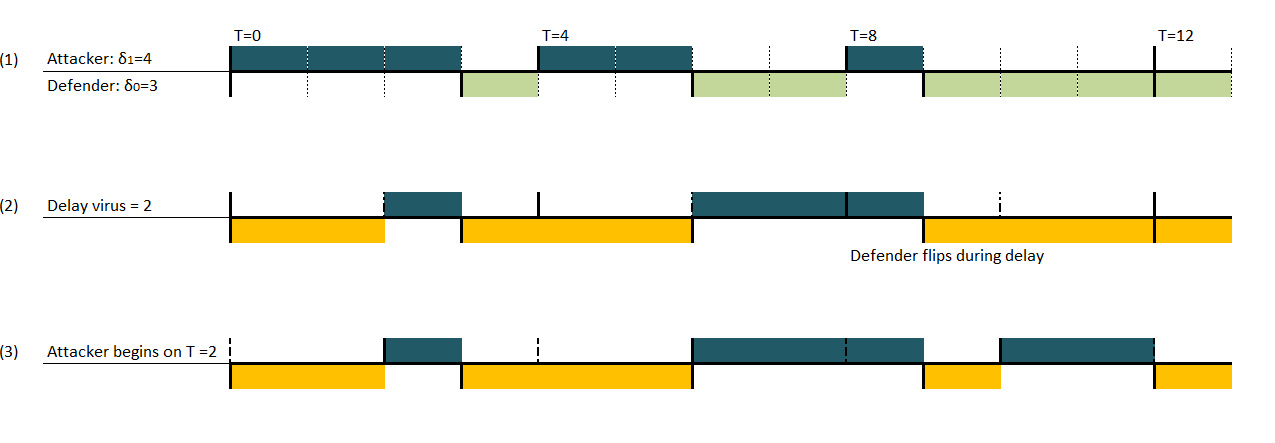
\includegraphics[scale=0.3]{Images/diffVirusDelay.jpg}
\end{figure}

If \textit{i} is an Irrational number:
$ i \neq \dfrac{a}{b}$ with $b \in Z, a \in N$
Because we cannot write \textit{i} in a fraction, this means that we won't have a cycle. If we would have a cycle that means that we do have a number that divides \textit{i}. If we don't have a cycle it goes on forever. Meaning that it goes on to infinity. This also means that no number will be repeated two times. If it does that means that their is repetition, meaning again that their is a cycle. We can conclude that if we have no cycle and no number will be repeated twice, that it will enumerate every number between 0 and the biggest interval. \todo{interval definieren}
Even though time is continious, irrational numbers are not considered. We kunnen continue tijd voldoende dicht benaderen door enkel rationele getallen in beschouwing te nemen. Vlakbij elk Irrationaal getal ligt immers een Rationaal getal.

A $\delta$ that is irrational will have no cycle. 





%%% Local Variables: 
%%% mode: latex
%%% TeX-master: "thesis"
%%% End: 



%\chapter{APT}
\label{cha:7}
%\documentclass[10pt]{article}\

%%%%%%%%%%%%%%%%%%%%%%%%%%%%%%%%%%%%%%%%%%%%%%%%%%%%%%%%%%
%%%%%			Introduction Chapter 7			%%%%%%
%%%%%												%%%%%%
%%%%%												%%%%%%
%%%%%%%%%%%%%%%%%%%%%%%%%%%%%%%%%%%%%%%%%%%%%%%%%%%%%%%%%%


\section{Advanced Persistent Threats}

A targeted attack follows most of the time a serie of stages to attack its victim. This pattern of stages is also know as the Kill Chain, first mentioned by .. []. An APT will not always follow exact each step of this chain but it will give a good guideline of how an APT works. 
\begin{enumerate}
\item \textbf{Reconnaissance}: During the first step of the Kill Chain an attacker will look for information to find an interesting victim. This information can be emailaddresses, IP addresses, conference information, anything that is available about the victim.
\item \textbf{Weaponization}: In the second stage the attacker will use an exploit and add a malicious playload to be send to the victim. 
\item \textbf{Delivery}: The attacker will deliver his malicious code to the victim through different kins of intrusion methods. This can include email, usb stick, cd's, web, applications or other means.
\item \textbf{Exploitation}:The attacker executes the exploit, which is only relevant if the attacker uses an exploit.
\item \textbf{Installation}: The malware will be installed on the asset. This is only relevant if the attacker uses malware as a part of the attack.
\item \textbf{Command and Control}: The attacker will set up a command and control channel for remote manipulation of the victim.
\item \textbf{Actions on Objectives}: With ''hands on keyboard'' access, intruders accomplish their original goal. 
\end{enumerate}
\todo{nog uitbreiden, toevoegen that attackers will stay unnoticed for as long as possible or leave unnoticed with sensitive information}


%\chapter{FlipIt with a virus propagation }
\label{cha:6}
%\documentclass[10pt]{article}\

%%%%%%%%%%%%%%%%%%%%%%%%%%%%%%%%%%%%%%%%%%%%%%%%%%%%%%%%%%
%%%%%			Introduction Chapter 6			%%%%%%
%%%%%												%%%%%%
%%%%%												%%%%%%
%%%%%%%%%%%%%%%%%%%%%%%%%%%%%%%%%%%%%%%%%%%%%%%%%%%%%%%%%%

\todo{resources vs nodes}
\section{Introduction}

%This section gives a formal definition of the FlipIt game with a virus propagation. First we derive a formula for a FlipIt game without a virus. After that we introduce a modification to this formula to achieve an adapted formula for a FlipIt game with a virus propagation. 
In this section we are going to elaborate how we are going to model a FlipIt game with multiple resources and a virus that propagates and infects the resources. First we derive a formula for a FlipIt game without a virus. After that we introduce a modification to this formula to achieve an adapted formula for a FlipIt game with a virus propagation. 
% We come up with a formula for the normal FlipIt (normal as in specific parameters and no normalising over the first interval) and then reform it to a FlipIt game with a virus. 

\subsection{FlipIt vs FlipIt with virus propagation}
Section [] explained the FlipIt game. This section will adapt a FlipIt game to a FlipIt game with virus propagation. We consider the non-adaptive continuous FlipIt game where both players play a periodic strategy with a random phase. De adaptation will be a game where the single resource consist of a computer network with multiple nodes. One of the players, the defender, will try to defend his network. The defender will do this by flipping all the nodes of the network in every move he plays. The attacker, the other player, will try to infect all the nodes in the network. The attacker will do this by flipping the node in the graph that can infect all the nodes in the shortest time possible. The attacker will only gain the control over the resource when he infects all the nodes of the network. The defender in contrast will gain control over the whole network when it has control over at least one node in the network. \\
\todo{ergens vermelden waarom we deze case bespreken en niet waarbij de aanvaller niet periodisch speelt}

After dropping a virus on the first resource, it takes a while for the virus to infect the entire network. The time that it takes for the virus to infect every node will be denoted as parameter \textit{d}. If we want to measure how long it takes for the virus to infect all the nodes in the network, we have to calculate the shortest path from the first infected node to the farthest node. This can be measured by a method that we will explain in section []. Using this parameter, a FlipIt game with virus propagation can be modelled. \\ 




%If the attacker attacks with the virus, the propagation will cause a delay of length \textit{d} before the attacker gains control over the whole network. This means that the gain of the attacker from the normal game has to be substracted with a delay every time the attacker moves. This game, where the attacker drops a virus, cannot be modelled completely by a FlipIt game with a delay. It may happen that the delay \textit{d} is bigger than the initial amount of control of the attacker. In this case the attacker will gain no control. If it would be with the delay caused by a phase bigger than zero the attacker would gain control after the defender flipt again. This is explained in figure \ref{fig:virusflip}. In the next section a formal definition .. \todo{verder uitleggen nog. Phases zijn vooraf uitgelegd.}




\subsection{define formula}
%The game FlipIt with a virus propagation is a two-player game with multiple resources. The multiple resources represent the nodes in a network. One of the players, the defender, will try to defend his network. The defender will do this by flipping all the nodes of the network in every move he plays. The attacker, the other player, will try to infect all the nodes in the network. The attacker will do this by flipping the node in the graph that can infect all the nodes in the shortest time possible. The attacker will gain the control over the network when all the resources are infected. So parameter \textit{d} will be the time of the shortest path from the start node to the furthest node. \\


\todo{deze sectie herschrijven}
There is a definition given for the gain of a player \textit{i} by the writers of the paper FlipIt [], but we want to add the property of a virus propagation to the game, hence parameter \textit{d}, so we are trying to find another formula that defines a game by counting the amount of time one of the players has control. \\
\todo{we hebben een periodisch spel, simpelste spel.}


\todo{zeggen dat we eerst de functie voorstellen van de normale FlipIt}
First a list of notations that will be used throughout the formal definition (see figure \ref{fig:notations} for a graphic representation of some of the notations):
\begin{description}
\item $\delta_{0}$: Positive and non zero number. This is the period of the defender. This denotes the length of the interval between two consecutive moves of the defender. 
\item $\delta_{1}$: This is the period of the attacker. This denotes the length of the interval between two consecutive moves of the attacker.
\item \textit{$T_{0}$}: This denotes the phase of the defender that was random and uniform chosen over the interval [0,$\delta_{0}$].
\item \textit{$T_{1}$}: This denotes the phase of the attacker that was chosen uniformly at random in interval [0,$\delta_{1}$].
\item \textit{Unit of control}: Defined as the period between gaining control and losing control over the resource.  
\item \textit{n}: n is the n'th interval of the attacker, starting from interval 1.
\item $\Delta A$ : This is a function that denotes the length of a unit of control of the attacker in the n'th interval of the attacker.
\item \textit{d}: Amount of time that the virus needs to infect every node in the network.
\item \textit{lcm(a,b)}: The \textit{lcm} of a and b is the least common multiple of a and b.
\item \textit{gcd(a,b)}: The \textit{gcd} of a and b is the greatest common divider of a and b.
\item \textit{Gain}:  The gain of a player is defined as the total amount of time that a player has owned the resource since the start of the game. In the context of a FlipIt game with virus propagation, the whole network is seen as one resource. This resource is owned by the attacked if he has control over the entire network. If the defender owns at least one node, he owns the resource.\\
\item \textit{Average Gain}:  $\gamma_{i}(t) = G_{i}(t)/t$ is the average gain rate of player \textit{i} which is defined as the fraction of time that player \textit{i} has control over the resource up to time t.
\item \textit{Benefit}: The average benefit of a player \textit{i} is denoted by $\beta_{i}(t) = \gamma_{i}(t) - k_{i} / \delta_{i}$, which is equal to the fraction of time that the resource has been owned by player \textit{i}, minus the cost rate for moving. For now we consider the cost rate equal to 0. In the rest of the paper the average benefit will be addressed as the benefit of the game for player \textit{i}.
\end{description}
\begin{figure}[hbtp]
\caption{Defining unit of control}
\centering
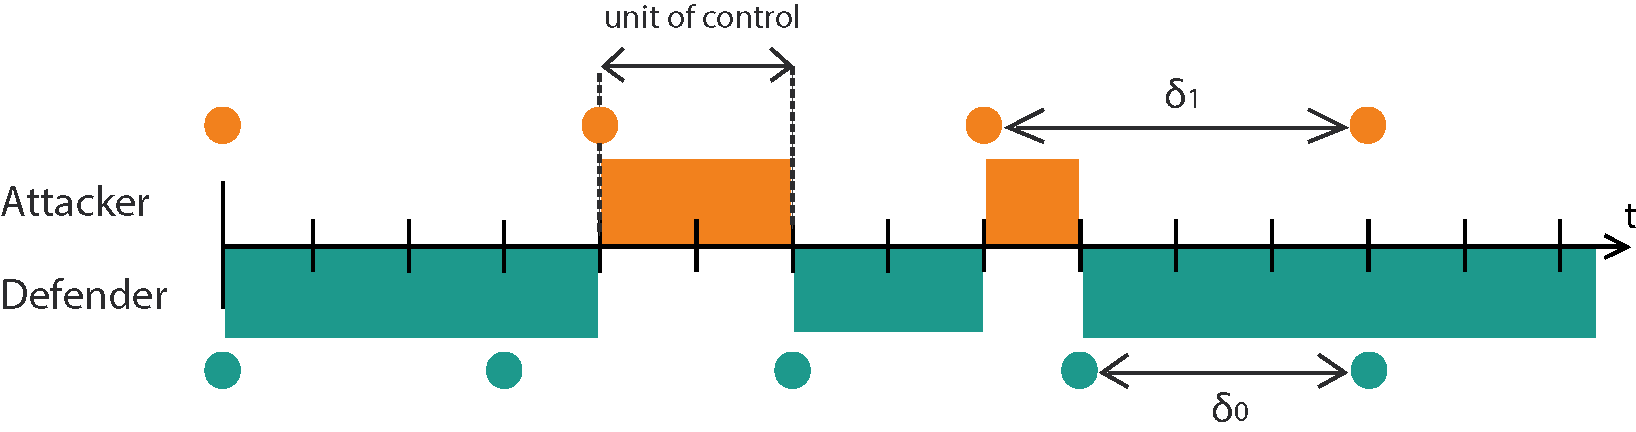
\includegraphics[scale=1]{Images/FlipSpel.png}
\label{fig:notations}
\end{figure}


%\begin{equation}\label{first}
%n = \delta_{1} mod \delta_{0}
%\end{equation}
%
%\begin{equation}\label{first}
%\Delta A = [( \delta_{0} - n + 1 ) * \delta_{1}] mod \delta_{1}
%\end{equation}
%
%\begin{equation}\label{first}
%\sum_{i=0}^{\delta_{1}} \lbrace [( \delta_{0} - i + 1 ) * \delta_{1}] mod \delta_{1} \rbrace
%\end{equation}
%\todo{formule met i nakijken}


\todo{We mag gebruikt worden in een wetenschappelijke tekst zolang de focus blijft op het werk en niet op de schrijver, FlipIt schrijvers gebruiken ook veel de we vorm} 
We start by computing the gain of the attacker in a periodic game without phases. Two cases are considered: case 1 where the defender moves as least as fast as the attacker and case 2 where the attacker plays as least as fast as the defender. After that we introduce the phases. Next we adapt our gain calculation to include virus propagation. Finally we compute the benefit of the attacker in function of the gain.   
\\
\subsubsection{Computing the gain for an attacker of a normal FlipIt game}
\textbf{Case  1:} \\
For $\delta_{1} > \delta_{0}$ (The defender moves faster than the attacker.) \\

We consider a game in which both of the players start with a phase $T_{0}$ and phase $T_{1}$ equal to zero. Both players start their first move at $t=0$. As previously stated (in the formal definition of the game and the introduction of different notations used throughout the paper), the defender has control in the beginning of the game at $t=0$. If the two players move at the same time during the game, the moves cancel and no change of state happens. \\ \todo{eerder gedefinieerd dat elk spel begint op t=0}

To compute the gain formula for the attacker, we need to calculate the amount of time that the attacker has control over the game from the start of the game up to time t. This can be done by computing all the units of control of the attacker up to time t \todo{formule is niet in staat om dat te doen als functie van t} and summing them. \\
The formula that we are going to compute will not be in function of the time but in function of the intervals of the attacker. By doing this we always have a whole unit of control. If time is used the last unit of control can be shortened. Because the game goes on indefinitely and because it is easier to compute a formula in function of the intervals of the attacker, the gain formula will be in function of the intervals of the attacker. \todo{kan misschien beter uitgelegd worden}

For that reason we divide our time line of our FlipIt game into different intervals of size $\delta_{1}$. Therefore every time the attacker moves we have the start of a new interval. Considering that the defender will move faster than the attacker, he or she will at least move one time during the interval of the attacker. Because the attacker only moves at the start of his or her interval we can say that the defender will always end as being in control of the resource. \todo{tekening met voorbeeld}. To calculate how long the unit of control of the attacker is in the n'th interval, we only need to know how long the attacker has control over the resource before the defender moves in that interval. First we need to calculate the start time of the n'th interval which will be a multiple of the period of the attacker. Once we know this we need to know what the difference is between this amount of time and the amount of time when the defender will flip. To do this we take the modulo of the negative of the amount of time of the attacker with the period of the defender. By doing so we calculate how much it takes to add to this time to compleet to a time that is a multiplier of the period of the defender. See figure \ref{fig:modulo} to see a graphic representation of this modulo. 
\todo{blabla en dan hebben we de volgende formule}
\begin{figure}[hbtp]
\caption{Taking the modulo of a negative number}
\centering
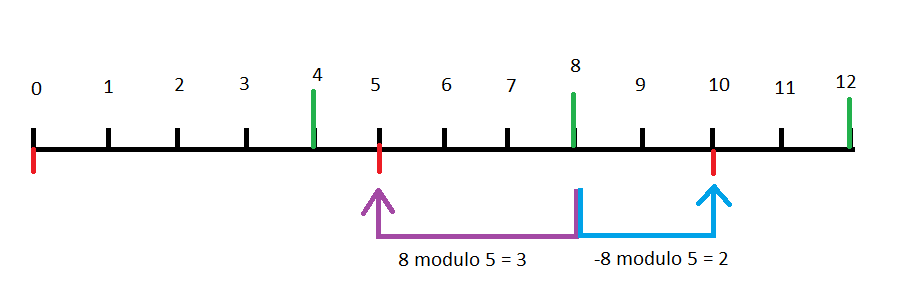
\includegraphics[scale=0.6]{Images/Modulo.png}
\label{fig:modulo}
\end{figure}

\todo{modulo uitleggen en dan verder door tot deze formule}
This brings us to the next forumula to calculate the length of a unit of control in the n'th interval of the attacker. 
\todo{definieer dat delta groter als nul is en niet negatief}
For every positive and non zero real $\delta_{1}$ and $\delta_{0}$ $\in$ \(\mathbb{R}\) and every n $\in$ \(\mathbb{N}\) (including 0 in the set of natural numbers) :
\begin{equation}\label{first}
\Delta A = [( 1- n  ) \cdot \delta_{1}] mod \delta_{0}
\end{equation}
where n is the number of the n'th interval of the attacker where the length of the unit of control of the attacker is calculated.\\

%In this formula we multiply the number of unit of control that we want with the period of Attacker ( $\delta_{1}$). 
The 1 - n is when we count beginning from 1. If we start counting starting at 0 we leave the 1 and the formula becomes:
\begin{equation}\label{first}
\Delta A = [( - n  ) \cdot \delta_{1}] mod \delta_{0}
\end{equation}

%We know that each interval ends with the control for the defender. This means that we only need to know how long the defender had control during that interval and take the rest. The rest will be the amount of time the attacker has control in that interval. We take the rest by doing the $mod \delta_{0} $

For phases .. \\

\textbf{Case 2}:
Alles omdraaien \todo{beter beschrijven}



\subsection{Formula with a virus propagation}
Now we can define how we can use the previous formula to calculate the gain of the attacker in a FlipIt game with virus propagation.
As mentioned before parameter \textit{d} defines the virus propagation. It will take an amount of time \textit{d} before the attacker gains control over all the resources. In the previous section we defined a formula to calculate each unit of control of the attacker. If the virus propagation takes \textit{d} time before every resource is infected then this d has to be subtracted from each unit of control. (see figure \ref{fig:virusflip}). It may happen that the unit of control is less than \textit{d}. The result of the substration will be a negative number in time. In this case this means that the defender has flipped all the resources before the attacker could gain control over all the resources. To calculate the gain only the units of control bigger than 0 have to be summarized. So the formula becomes:

\begin{equation}\label{first}
Gain_{1} = \sum_{i=0}^{\delta_{0}} \lbrace [( 1 - i ) \cdot \delta_{1}] mod \delta_{0} - d \rbrace  > 0 \rbrace 
\end{equation}

\begin{figure}[hbtp]
\caption{Difference in a FlipIt game between delay caused by a virus and a phase bigger than zero for the Attacker}
\centering
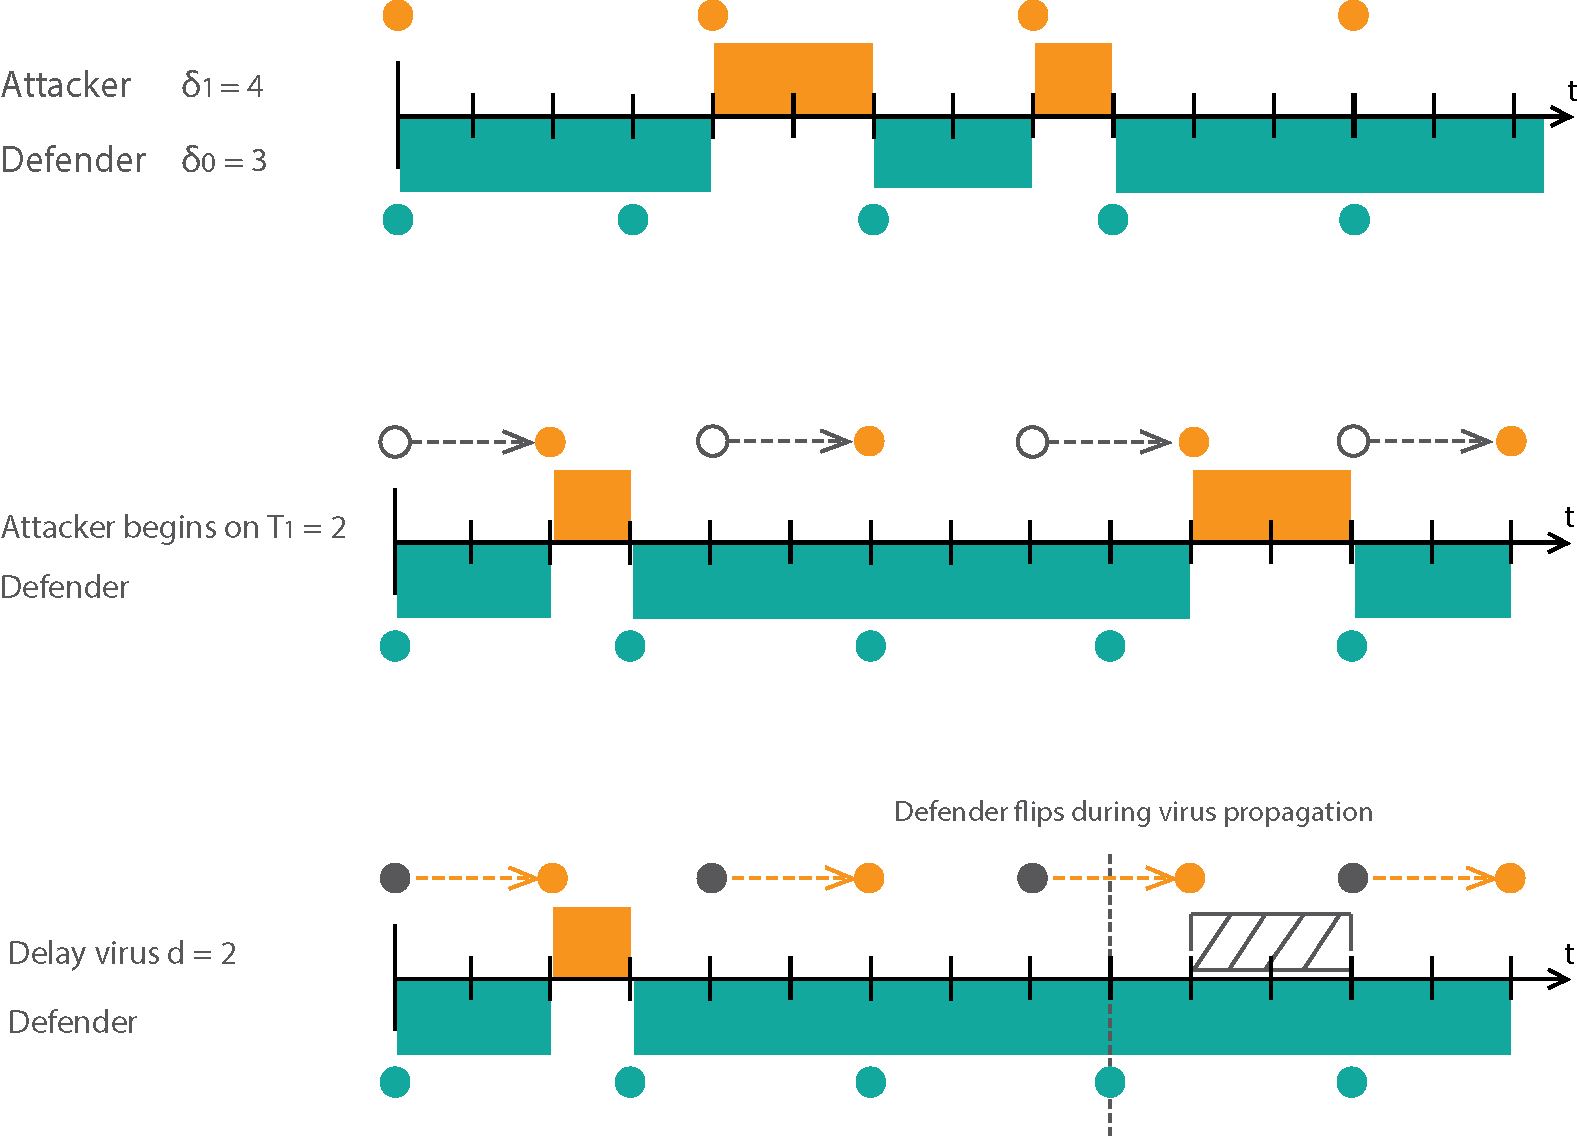
\includegraphics[scale=1]{Images/Flipvirus}
\label{fig:virusflip}
\end{figure}


\subsubsection{Computing the benefit of a FLipIt game with virus propagation}

To be able to calculate the benefit of the attacker, we need to calculate the average gain rate of the attacker. We will look at this for two cases. One case where $\delta_{0}$ and $\delta_{1}$ $\in$ \(\mathbb{Q}\) and the other one where $\delta_{0}$ and $\delta_{1}$ $\in$ \(\mathbb{I}.\) \\

\textbf{Rational numbers (\(\mathbb{Q}\)):} For $\delta_{0}$ and $\delta_{1}$ $\in$ \(\mathbb{Q}\), a repetition of the game will occur. As every rational number is any number that can be expressed as the fraction p/q with p and q $\in$ \(\mathbb{Z}\) (integers), with the denominator q not equal to zero, it is possible to find the \textit{lcm} of $\delta_{0}$ and $\delta_{1}$. The \textit{lcm} is defined for all rational numbers as: $lcm(\dfrac{a}{b},\dfrac{c}{d})= \dfrac{a \cdot c}{gcd(b,d)} with  $ [\todo{referentie}]. When \textit{t} is equal to the \textit{lcm} of $\delta_{0}$ and $\delta_{1}$, both players will move again at the same time and this can be mapped to the beginning of the game. Because we stated that at the end of the interval of the attacker, the defender is in control and because if two players move at the same time the moves are cancelled, we can map this to the beginning of the game. Since the game goes on infinite, to calculate the average gain of the attacker, it is sufficient to calculate the average gain of the attacker only during this repetition equal to the \textit{lcm} of $\delta_{0}$ and $\delta_{1}$. 
%This means that if we want to calculate the gain of the attacker we need to calculate the time the attacker has control over the total amount of time that has passed by.
%For $\delta_{0}$ and $\delta_{1}$ $\in$ \(\mathbb{Q}\) we can see that we have a cycle. A pattern that comes back over and over again. That is when the amount of time is a multiple of $\delta_{0}$ and $\delta_{1}$ or the largest common multiplier (\textit{lcm}). At this point the Attacker and the Defender move at the same time what brings us back to the beginning.
So to calculate the gain of $\delta_{0}$ and $\delta_{1}$ $\in$ \(\mathbb{Q}\) we need to calculate the amount of control units of the attacker that go into the length of time units equal to the \textit{lcm} of  $\delta_{0}$ and $\delta_{1}$. This will be equal to the amount of time that the period of the attacker goes into the \textit{lcm}. We denote this by parameter \textit{p} and define it as follow:
\begin{equation}\label{first}
p = \dfrac{lcm(\delta_{0},\delta_{1})}{\delta_{1} } 
\end{equation}
After this calculation we summarize our units of control in function of \textit{p} and divide it by the \textit{lcm} of $\delta_{0} $ and $ \delta_{1}$, which is the total amount of time for one cycle.  This gives us the following formula of the benefit of the attacker with a cost rate equal to zero:

\begin{equation}\label{first}
\beta_{1} = \dfrac{\sum_{i=0}^{p} \lbrace [( 1 - i ) \cdot \delta_{1}] mod \delta_{0} \rbrace }{lcm(\delta_{0},\delta_{1})} 
\end{equation}

%We can also define a formula without the greatest common divider. Every $\delta_{0}$ and $\delta_{1}$ have to be written in a fraction:
%\begin{equation}\label{first}
%\delta_{0}=\dfrac{a}{b} ~~~~and~~~~\delta_{1}=\dfrac{c}{d}
%\end{equation}
%If  $\delta_{0}$ or $\delta_{1}$ is a Geheel getal then b or d will be 1. The formula for the gain becomes different:\\
%
%\todo{formule zoeken zonder lcm en gcd}


\textbf{Irrational numbers (\(\mathbb{I}\)):} If $\delta_{0}$ and/or $\delta_{1}$ $\in$ \(\mathbb{I}\):
An irrational number $ i \neq \dfrac{a}{b}$ with $b \in$ \(\mathbb{Z}\) , a $\in$ \(\mathbb{N}\).
Because we cannot write \textit{i} as a fraction, this means that we cannot compute a common multiplier of $\delta_{0}$ and $\delta_{1}$. If their is no common multiplier the attacker and the defender won't move at one point on the same time, meaning that this does not result in a cycle. If we would have a cycle that means that there exists a number \textit{x} that can be divided by $\delta_{0}$ and $\delta_{1}$. At $t=x$ both of the players will move at the same time, which is not possible because then their would be a cycle. Since their is no cycle it also means that no unit of control will be repeated two times. Every unit of control will have a distinct length. If it does that means that their is repetition, meaning again that their is a cycle. \todo{nog verder uitleggen} We can conclude that if we have no cycle and no number will be repeated twice, that it will enumerate every number between 0 and the biggest interval (which is $\delta_{0}$). 
\textit{The reals are uncountable; that is: while both the set of all natural numbers and the set of all real numbers are infinite sets, there can be no one-to-one function from the real numbers to the natural numbers} [WikiPedia: real numbers] If they are uncountable that means that we cannot calculate the sum of all the numbers between 0 and the biggest interval. This is proved by the Cantor diagonalisation argument. Uncountable does not mean that we cannot order it. The Field of the real numbers is ordered. 

What we can do is take the limit, count as many control units of time of the attacker and divide it by the greatest amount of time. We can see that this eventually will result to the solution given by the writers of FlipIt. [r/2]. Example delta1 Pi and delta0 1. Grafiek voor maken.

%\subsection{Random phase}
%For now we assumed that the first move of both players started at phase $t=0$. In the FlipIt game the first move is chosen uniformly over the interval [0,$\delta$]. We will call this first move the phase move and denote it by $T_{1}$ for the attacker and $T_{0}$ for the defender.
%We will have to integrate these two phases into the formula.  
%\begin{equation}      
%\boxed{\eta \leq C(\delta(\eta) +\Lambda_M(0,\delta))}
%\end{equation}
%
%\begin{equation}\label{first}
%a=b+c
%\end{equation}
%
%\begin{subequations}\label{grp}
%\begin{align}
%a&=b+c\label{second}\\
%d&=e+f+g\label{third}\\
%h&=i+j\label{fourth}
%\end{align}
%\end{subequations}



%%% Local Variables: 
%%% mode: latex
%%% TeX-master: "thesis"
%%% End: 



%\chapter{FlipIt game with virus propagation}
\label{chapter2:FlipIt with virus propagation}
%\documentclass[10pt]{article}
%\begin{document}

%%%%%%%%%%%%%%%%%%%%%%%%%%%%%%%%%%%%%%%%%%%%%%%%%%%%%%%%%%
%%%%%			Introduction Chapter 1				%%%%%%
%%%%%												%%%%%%
%%%%%												%%%%%%
%%%%%%%%%%%%%%%%%%%%%%%%%%%%%%%%%%%%%%%%%%%%%%%%%%%%%%%%%%

\section{Introduction}
\label{Ch2:Intro}
The game of FlipIt with virus propagation considers attackers where their moves are not instantaneous. This can be motivated by an example of a virus. A virus can be dropped on a network but it only compromises the whole network if every node in the network is infected. The basic FlipIt game does not take this into account. In this chapter the FlipIt game with virus propagation is explained and how it can be modelled. First the main differences with the basic FlipIt game are discussed in section \ref{ch2:diffFlip}. Next in section \ref{ch2:formal} the formal definition of the game with virus propagation is given. At last, in section \ref{ch2:periodicvirus} a periodic strategy game is considered and the formalization of the formulas with virus propagation are determined.\\

This chapter explains how to model a FlipIt game with a virus propagation that infects a network. The first section explains the difference between a normal FlipIt game and a FlipIt game with virus propagation. The next section derives a formula to calculate the benefit for a FlipIt game with a virus propagation. In the last section we calculate the Nash equilibrium for the benefit formula.
\section{FlipIt game with virus propagation}

Welke aanpassing en motivatie: attacker 1 speler die elke keer virus probeert te droppen. Defender die elke keer patcht als er virus gedropt wordt. Elke patch voldoet aan de meest recente patch dus alle virussen die ook gedropt zijn worden weggedaan. Voor future work: patch systeem aanpassen. 

The actions of a defender: the actions of an attacker:

\section{Explaining difference between FlipIt with and without virus propagation}
\label{ch2:diffFlip}
\begin{figure}[hbtp]
\caption{The first game is the basic FlipIt game. The second is a FlipIt game with a delay. During the first flip of the attacker, the defender moves after the delay, causing the attacker to get control over the resource. During the second flip of the attacker, the defender flips at time t+d, causing the defender to take control over the resource before the attacker. During the third and final flip of the attacker, the defender flips during time t+d, causing the attacker to never gain control over the resource. }
\centering
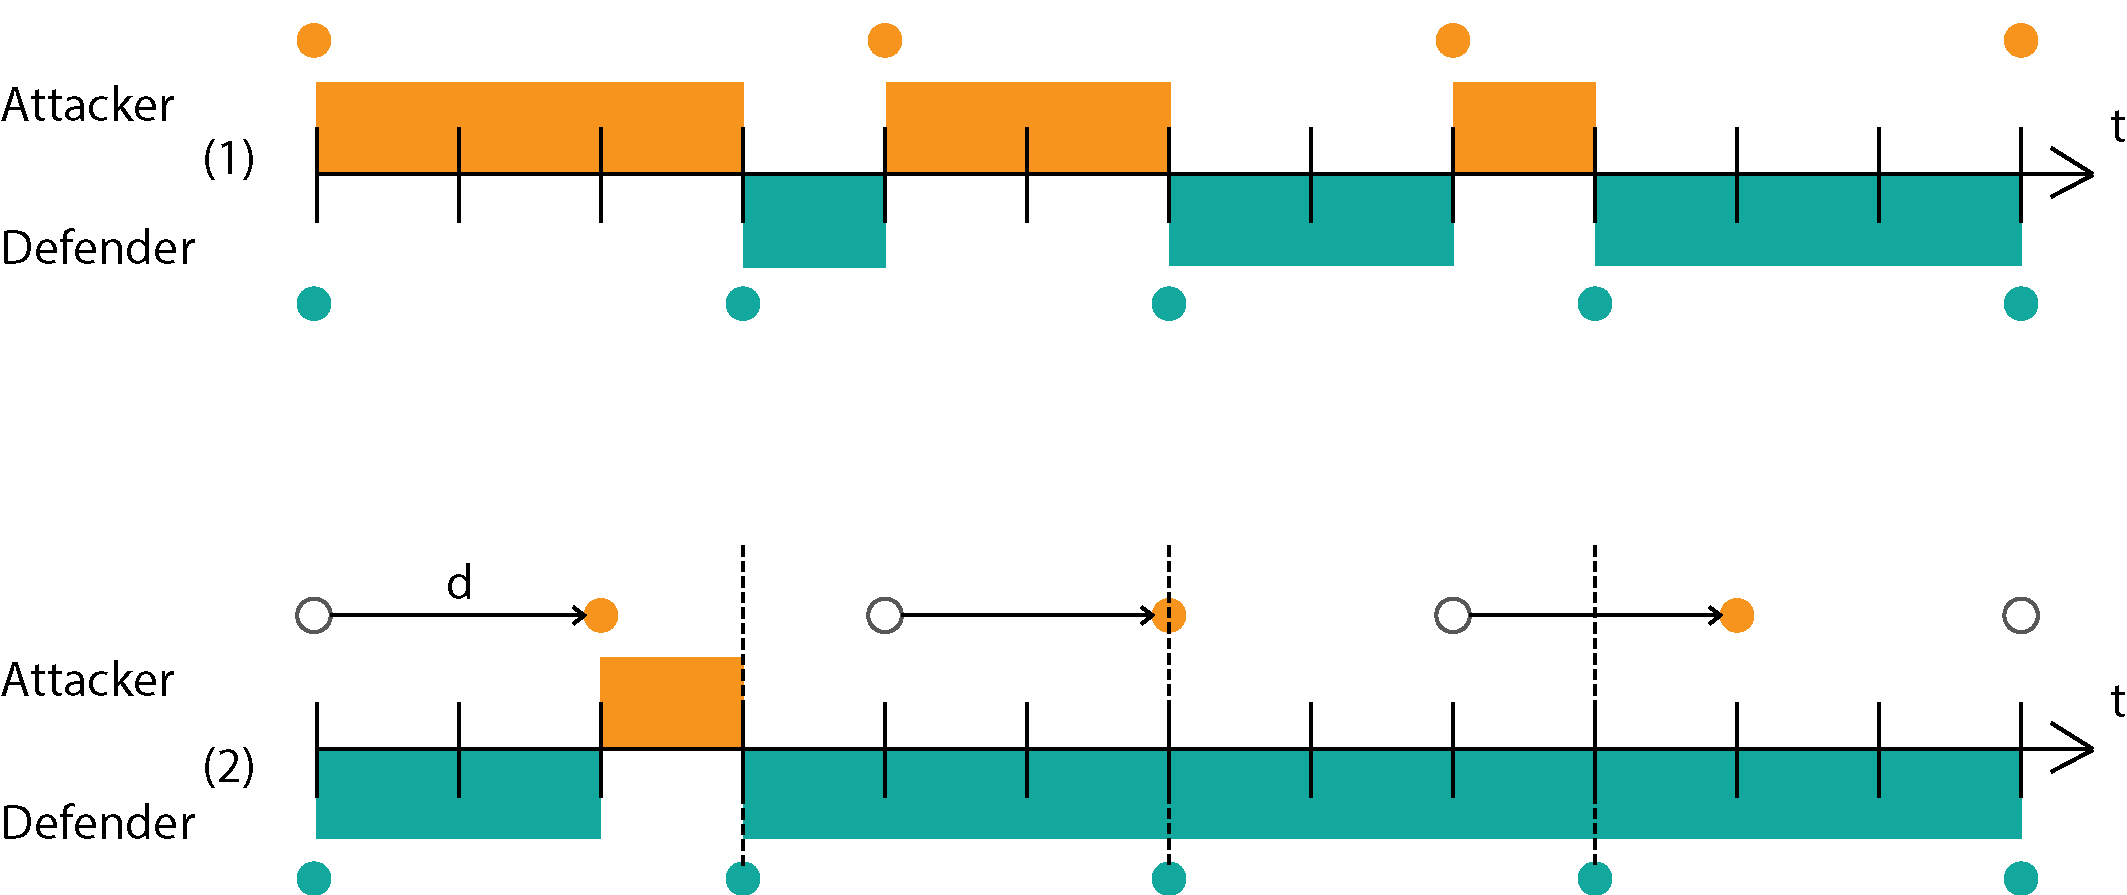
\includegraphics[scale=0.7]{Images/dtFlip.png}
\label{dt}
\end{figure}

A FlipIt game consists of a single resource. To represent the security problem, the game now defines its single resource as a computer network with multiple
nodes. One of the players, the defender, will try to defend his network. The defender
will do this by flipping all the nodes of the network (i.e. the entire resource) in every move he plays. The
attacker on the other hand will try to infect all the nodes in the network. The attacker
will do this by flipping the node in the graph that can infect all the nodes in the
shortest possible time. After dropping a virus on the first node, it takes a while for the virus to infect the entire network. Since the original FlipIt game works with a single resource that is always flipped entirely, the assumption is made that the attacker is considered to gain immediate full control over the resource when the network has been infected, even it is only one node that has been infected.\\

In reality however, after dropping a virus on the first node, it takes a while for the virus to infect
the entire network. So, the assumption that the attacker has full control over the resource as soon as a node has been infected, is not realistic. The attacker has only control of the network once all or a sufficient number of nodes are infected. 
The time that it takes for the virus to infect every node (or a sufficient number of nodes) will be
denoted as an infection-delay variable \textit{d} (called 'delay' for short in the remainder of this paper). If we want to measure how long it takes for the virus to
infect all the nodes in the network, we have to calculate the shortest path from the
first infected node to the farthest node. Rather than denoting the time needed for infecting \textit{all} the nodes, the variable $d$ can also be used to denote the time needed to infect \textit{a sufficient number} of nodes.

Assume that an attacker attacks at time \textit{t}, he doesn't get immediate control over the resource, but he only gains control at time \textit{t + d}, with $d$ denoting the time needed to infect a sufficiently number (or all) nodes. If the defender flips the network before the period $d$ has elapsed (so, somewhere between $t$ and $t + d$), then the attacker will never gain full control over the resource. See figure \ref{dt}. This implies that the mathematical formulas for gain and benefit need to be adapted to the fact that the attacker loses part of its benefit because of this delay. In the remainder of this paper, we will adapt the formalization of the FlipIt game using the variable $d$. \\ 


%%------------------------------------------------%
%%            Intro Game Theory 					 %
%%------------------------------------------------%
%\subsection{Actions of the attacker}
%A virus has different kind of ways of making his way through a company network. We will describe the different ways of how the virus can propagate. For start we will say that the virus or worm will be dropped on Node i and that it has k numbers of neighbours. 
%\begin{enumerate}
%\item Node i is infected and will spread the virus or worm to every k neighbours and will stop infecting the neighbours in the next step
%\item Node i is infected and will spread the virus or worm to every k neighbours and will keep on spreading the virus to the same neighbours in every next step
%\item Node i is infected and will spread the virus to only one of the k neighbours and will stop infecting another neighbour in the next step
%\item Node i is infected and will spread the virus to only one of the k neighbours and in the next step it will infect another one of the k neighbours 
%\end{enumerate}
%
%In the game that will be modelled in the paper we will use the settings of the first spreading method. We will not use method 2 because this kind of propagation will float the network. Because we use the settings of a mail system and contact in a mailing list the method of 3 and 4 are not used. \\
%In the first method the node that has been infected can be again infected. If one of the neighbours infects the node again the node will infect his neighbours again. By using this spreading method we have three distinct states in which a node can be situated. An \textit{infected state}, a \textit{clean state} and a \textit{spreading state}. An infected state means that the node is infected and will not spread the virus to its neighbours, a clean state means that the node is not infected on that moment and a spreading state means that the node is infected and that it will spread the virus or worm to its neighbours in the next step.
%We can argument this kind of propagation through a mail worm. \todo{voorbeeld geven van zo een worm}
%%Another propagation method is that the virus works as a token. It will propagate to only one neighbour and continue to spread. 
%
%The Attacker itself has two different ways of attacking the company network. It will only infected one node of the network and will wait for the virus to spread itself through the network. We will model two ways of attacks of an Attacker:
%\begin{enumerate}
%\item The attacker drops the virus on a random node on the network
%\item The attacker drops the virus on a targeted node on the network
%\end{enumerate}
%The attacker in this game will put a virus or worm on one of the nodes in the network. (This will happen at random.) The attacker does not know on which node the virus will be dropped. We will use this randomness because \todo{feit uit security rapport symantec} most viruses are spread via a usb stick or a shared resource. If we use this spreading method where we have a targeted attack the attacker will have more information about the network. \\
%
%The attacker can choose at which rate it will drop a virus on one of the nodes on the network. The cost of dropping a virus will be the same. It will not increase. If it will increase this means that the attacker will eventually drop out of the game because it becomes to expensive.\\
%The attacker is in control over the game if it manages to infect a subset of all the resources of the company network.
%
%
%\subsection{Actions of the defender}
%The attacker wants to protect all the nodes of his network. It can do so by getting back control over the resources. We will assume that the defender of the network has knowledge over his own network. Which is convenient in the real world because a company has to know how his infrastructure looks like.\\
%
%The defender has two possible ways of defending its network:
%\begin{enumerate}
%\item The defender flips all the nodes of his network
%\item The defender will flip a subset of the nodes of his network
%\end{enumerate}
%
%The cost of flipping all the nods of the network will be greater than the cost of flipping a subset of nodes. We make this assumption because otherwise it will be beneficial for the defender to always flip all the nodes in the network.\\
%
%We will also make the assumption that as a defender flips a node the node can get infected again. A flip will not be  correlated to a patch but to a clean-up. \todo{waarom geen patch, wormen kunnen veranderen gaandeweg}
%\todo{andere mogelijkheid:} Another setting of the game can be that the flip of the defender is equal to a patch and that the resource cannot be infected any more. But with this case we deviate from the flipIt game, because the attacker cannot flip the resource any more. Unless we work with different virusses every time the attacker flips. We start with the less complex game of flipping is equal to a clean-up.




\section{Playing periodically with virus propagation}
\label{ch2:periodicvirus}




The formalization starts from the model of the non-adaptive continuous basic FlipIt game where players use a periodic strategy with a random phase. This choice is motivated by the assumption that in most organisations, the defence strategy is to periodically defend the network. This corresponds to a periodic defender strategy.  A periodic attacker strategy is assumed as well, to be able to compare the results with the periodic strategy of the FlipIt game in \cite{FlipIt}. %, as this also corresponds to a common real life strategy. %nog eventueel verder te motiveren
Further research can investigate the effect of relaxing this assumption. \\



Similarly as in \cite{FlipIt}, we split the formalization in two cases. The first case is where the defender plays at least as fast as the attacker, the second case is where the attacker plays at least as fast as the defender. For each of these cases, first the benefit formula of the basic case without delay is presented, and then the delay is introduced.  \\

Intuitively we could assume that $d$ can never be bigger than $\delta_{A}$ because then the benefit for the defender would always be 1. This is not always true. It is only true if $d$ is bigger than $\delta_{D}$, because then the defender will always be in control. For this we only calculate the formulas for the cases where $d$ is smaller than $\delta_{D}$. We can already conclude that it is no use for the attacker to play when the delay is bigger than $\delta_{D}$. \\

\subsection{Formalization the benefit formula including the infection-delay}



 A Periodic strategy is a non-adaptive renewal strategy where the time intervals between consecutive moves are a fixed period, denoted by $\delta$. Moreover it has a random phase, that is chosen uniformly and random in the interval $[0,\delta]$ for the first move. The average rate of play of a player is denoted by $\alpha_{i} = \dfrac{1}{\delta_{i}}$. List of symbols that will be used throughout the paper. Figure \ref{FlipItDelay} represents a couple of the symbols for clarification.\\
~~\\
\begin{figure}[hbtp]
\caption{Formalization of a FlipIt game with delay: A representation of a FlipIt game where both players are playing periodically. Every move or flip is indicated by a blue or orange circle.  The defender is represented in blue and plays with a period of $\delta_{D}$. The flip of the attacker is represented by a white circle, but because there is a delay d, the attacker only controls the resource after time d represented by an orange circle. The attacker plays with a period of $\delta_{A}$. The blue and orange rectangles represent the amount of time the respective player is in control of the resource.}
\centering
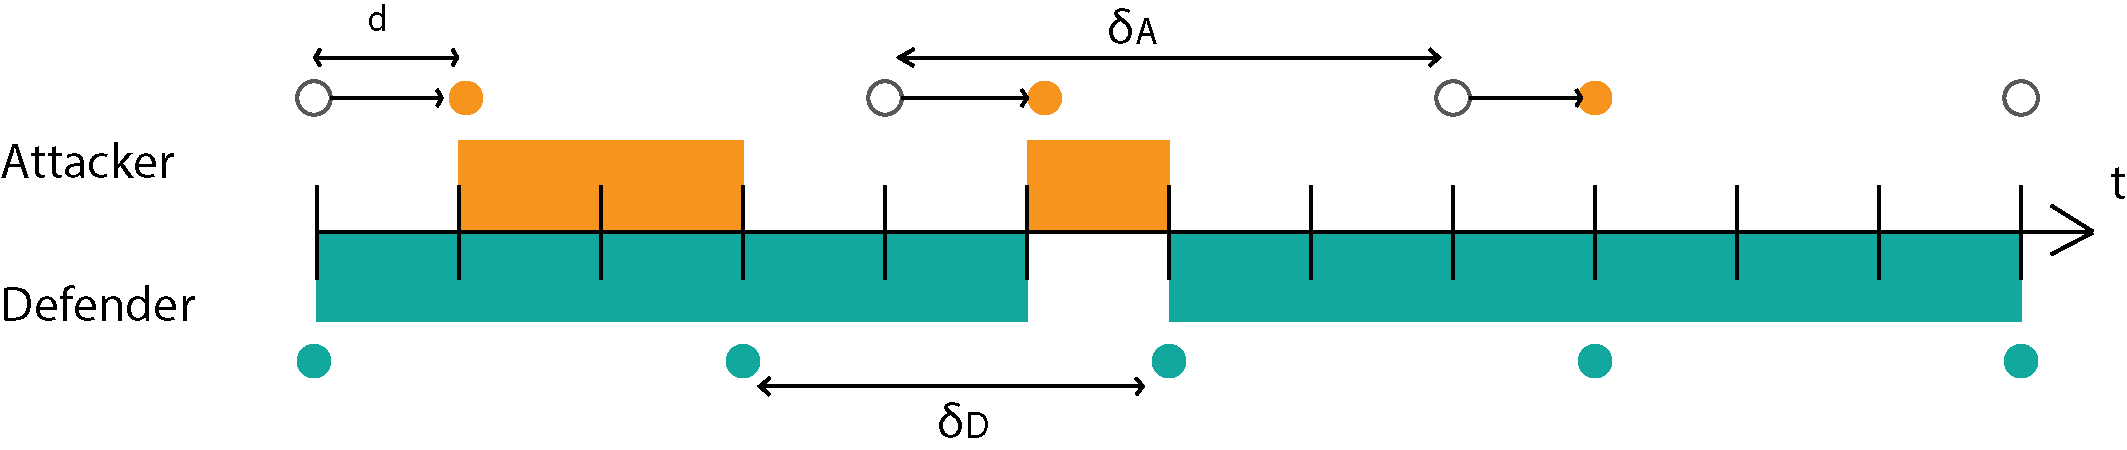
\includegraphics[scale=0.7]{Images/DefFlip.png}
\label{FlipItDelay}
\end{figure}

\begin{description}
\item $i$: Defines the player. Different as in the FlipIt paper where the defender is denoted by the subscript 0 and the attacker by the subscript 1.
\item $\delta_{i}$: The length of the interval between two consecutive moves of player \textit{i}. 
\item $\alpha_{i}$: The average flip rate of player \textit{i}, given by $\alpha_{i}=1/\delta_{i}$.
\item $k_{i}$: The cost of player \textit{i}'s moves.
\item $d$: The delay caused by the virus propagation.
\item $G_{i}(t)$: The total gain of player \textit{i} denotes the amount of time player \textit{i} is in control over the resource up to time \textit{t}.
\item $\gamma_{i}$: The average gain rate of player \textit{i} defined as $G_{i}(t)/t$
\item $\beta_{i}$:  The average benefit rate up to time \textit{t} defined as  $\beta_{i} = \gamma_{i} -k_{i} \alpha_{i} $.
\item $opt_{i}$: The optimum function.
\end{description}




\subsection*{\textbf{Case 1:} $\delta_{D} \leq \delta_{A} $ (The defender plays at least as fast as the attacker.) }

Let $r = \dfrac{\delta_{D}}{ \delta_{A} }$. The intervals between two consecutive defender's moves have length $\delta_{D}$. Consider a given defender move interval. The probability over the attacker's phase selection that the attacker moves in this interval is r. Given that the attacker moves within the interval, he moves exactly once within the interval (since $\delta_{D} \leq \delta_{A} $) and his move is distributed uniformly at random. \\

The expected period of attacker control within the interval would be r/2, without considering the delay by a virus. Therefore the benefit for the attacker, without considering the delay, can be expressed as follows:

\begin{equation*}
\beta_{A}(\alpha_{D},\alpha_{A}) =\dfrac {r} {2} - k_{A} \alpha_{A} = \dfrac {\delta_{D}} {2\delta_{A}} - k_{A} \alpha_{A}  
\end{equation*}\\

Correspondingly, the benefit for the defender can be expressed as:
\begin{equation*}
\beta_{D}(\alpha_{D},\alpha_{A}) =1 -  \dfrac {r} {2} - k_{D} \alpha_{D} = 1 - \dfrac {\delta_{D}} {2\delta_{A}} - k_{D} \alpha_{D} 
\end{equation*}

\begin{figure}[hbtp]
\caption{Case 1: Difference between a basic FlipIt game and a FlipIt game with a delay. (1) is the FlipIt game without a delay and (2) is with a delay. The delay is denoted with an arrow. The attacker is only in control when the circle becomes orange.}
\centering
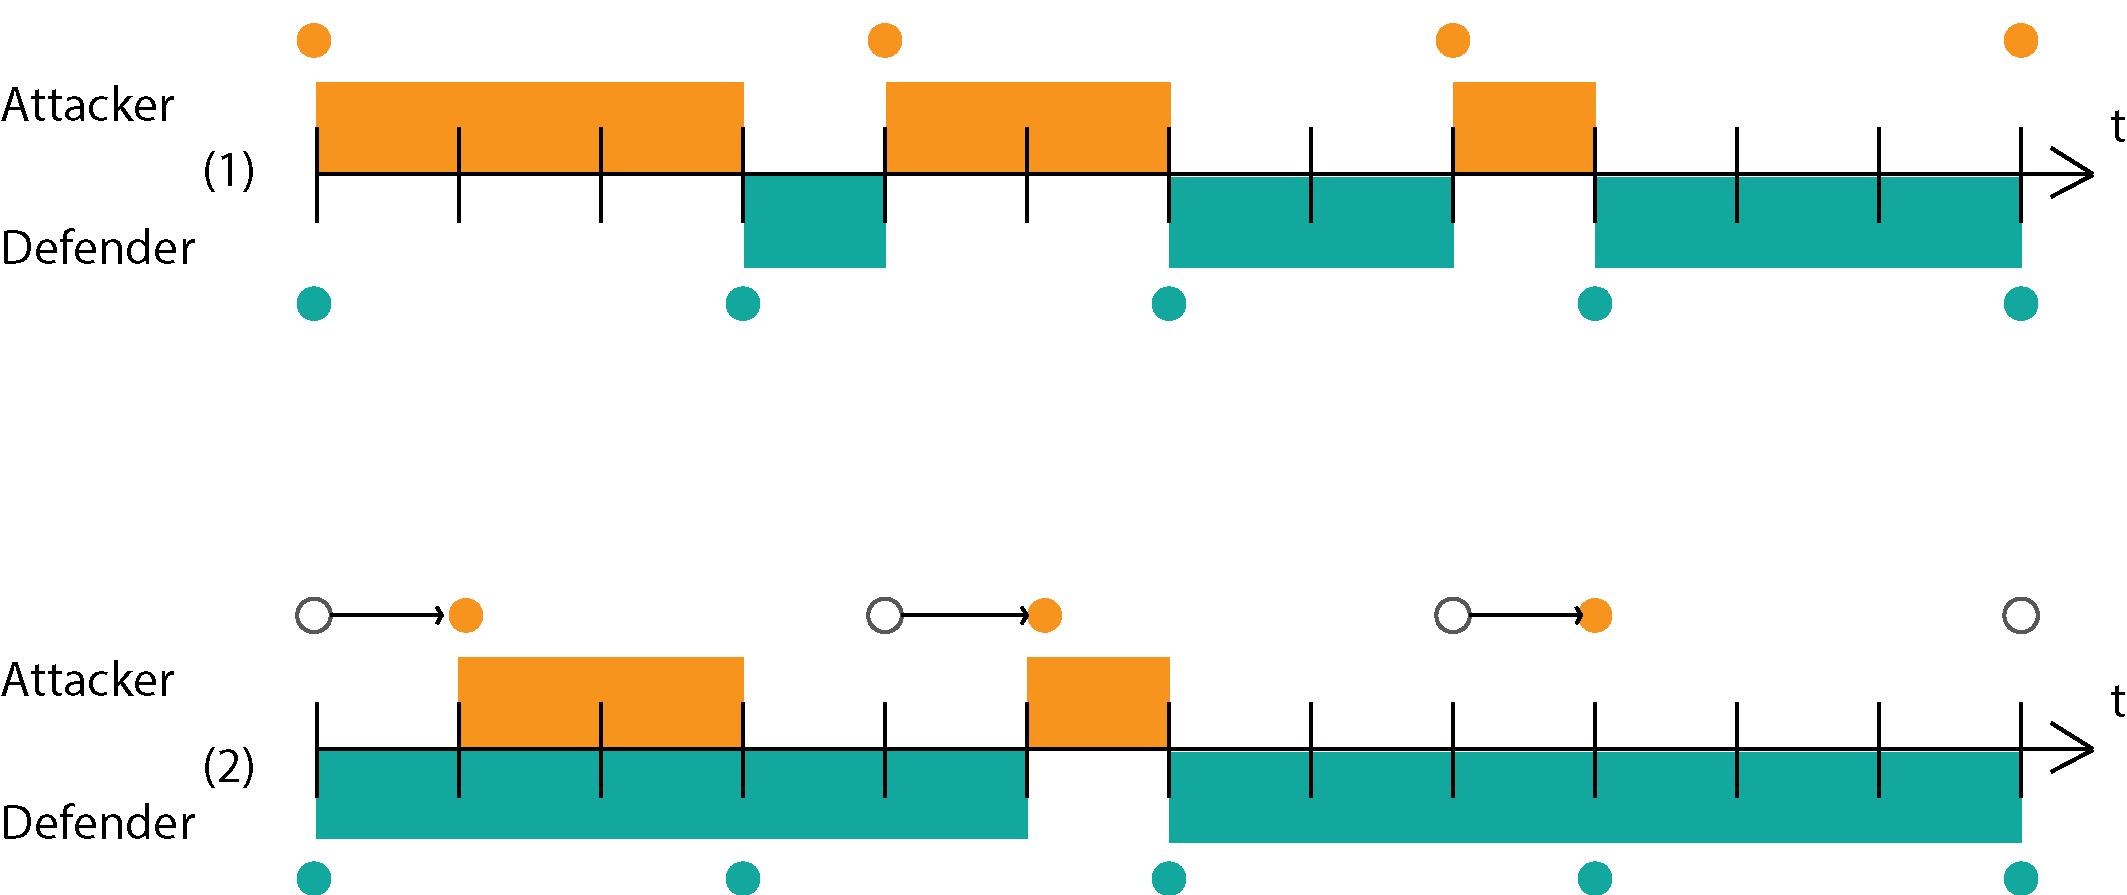
\includegraphics[scale=0.6]{../../doc/template/Images/DiffDelayCase1.png}
\label{fig:delaycase1}
\end{figure}


However, because of the delay required for virus propagation, the maximal time of control is reduced to $\delta_{D}-d$ , see figure \ref{fig:delaycase1}. There is a probability of \textit{r} that the attacker will move in the interval of the defender. However, the gain will not be half of the interval. Indeed, the attacker has to play soon enough to gain control, meaning that the attacker has to play during the period of $\delta_{D}-d$ during the interval of the defender. The probability that the attacker plays soon enough is $\dfrac{\delta_{D}-d}{\delta_{D}}$ and this will give the attacker an average gain of $\dfrac{\delta_{D}-d}{2}$. If the attacker moves after the period of $\delta_{D}-d$, the gain of the attacker will be zero. The probability that this happens is  $\dfrac{d}{\delta_{D}}$. The average gain rate of the attacker can then be expressed as follows if we look at one interval of the defender:
\begin{equation*}
\gamma_{A}(\alpha_{D},\alpha_{A}) = \dfrac {1}{\delta_{D}} [ \dfrac{\delta_{D}}{\delta_{A}} \cdot \dfrac{\delta_{D}-d}{\delta_{D}} \cdot \dfrac{\delta_{D}-d}{2} + \dfrac{\delta_{D}}{\delta_{A}} \cdot \dfrac{d}{\delta_{D}} \cdot 0 ]
\end{equation*}

To derive the benefit, the cost of moving is subtracted from the average gain. 
\begin{equation*}
\beta_{A}(\alpha_{D},\alpha_{A}) = \dfrac { (\delta_{D}-d) ^{2}} {2 \cdot \delta_{D}  \delta_{A}} - k_{A} \alpha_{A}
\end{equation*}
\begin{equation*}
\beta_{A}(\alpha_{D},\alpha_{A}) = \dfrac { \delta_{D}} {2 \cdot \delta_{A}} - k_{A} \alpha_{A} - ( \dfrac{d^{2}}{2 \cdot \delta_{A} \delta_{D}} - \dfrac{d}{\delta_{A}} )
\end{equation*}
 
 
 The benefit of the defender is expressed as follows:
\begin{equation*}
\beta_{D}(\alpha_{D},\alpha_{A}) = 1 - \dfrac { (\delta_{D}-d) ^{2}} {2 \cdot \delta_{D}  \delta_{A}} - k_{D} \alpha_{D}
\end{equation*}
~~\\
We can easily see that when $d$=0, we obtain the formula of the original FlipIt game.\\





\subsection*{\textbf{Case 2:} $\delta_{A} \leq \delta_{D} $ (The attacker plays at least as fast as the defender.) }

First let $r = \dfrac{\delta_{D}}{ \delta_{A} }$. The intervals between two consecutive attacker's moves have length $\delta_{A}$. Consider a given attackers move interval. The probability over the attacker's phase selection that the defender moves in this interval is $\dfrac{\delta_{A}}{ \delta_{D} } = (1/r)$. Given that the defender moves within the interval of the attacker, he moves exactly once within this interval (since $\delta_{A} \leq \delta_{D} $) and his move is distributed uniformly at random. \\

A similar analysis as in case 1 for a FlipIt game without virus propagation yields the following benefits:

\begin{equation*}
\beta_{D}(\alpha_{D},\alpha_{A}) = \dfrac {1} {2r} - k_{D} \alpha_{D} = \dfrac {\delta_{A}} {2\delta_{D}} - k_{D} \alpha_{D} 
\end{equation*}
\begin{equation*}
\beta_{A}(\alpha_{D},\alpha_{A}) =1 - \dfrac {1} {2r} - k_{A} \alpha_{A} = 1- \dfrac {\delta_{A}} {2\delta_{D}} - k_{A} \alpha_{A}  
\end{equation*}\\

An intuitive solution for the case with a virus would be to subtract the benefit of the attacker received in each interval with the delay similarly as in case 1. This would give us the following formula if we derive it in the same way:
\begin{equation*}
\beta_{A}=\dfrac{(\delta_{A} - d)^2}{2\delta_{A}\delta_{D}} - \dfrac{k_{A}}{\delta_{A}}
\end{equation*}

But this results in an overestimation. How closer $\delta_{A}/\delta_{D}$ is equal to one, the better the approximation. If $\delta_{A}/\delta_{D} = 1$ the result is correct. This formula does not take into account that if the attacker was in control in the previous interval, the delay should not be subtracted, because the delay will not be in control of the defender. This means that we have to look at what happens in the previous interval. \\

From the defender we know that his moves are instantaneous. It is easier to calculate the benefit of the defender in this case. Because the defender moves slower than the attacker we know that if the defender moves during the interval of the attacker, he only moves once within this interval.
The defender will move during the interval of the attacker with a probability of $\dfrac{\delta_{A}}{\delta_{D}} $. When this happens the defender will end with being in control at the end of the interval. In the next interval the attacker will have to regain control, meaning that during the delay, the defender stays in control, see figure \ref{fig:case2} cases (1) and (2). The defender will keep the control over the resource in the next interval over a period of the delay, namely \textit{d}. \\

Consider a timespan $\delta_{A} + d$, representing the attacker's interval followed by the delay period in his next interval. The defender will never move twice during this timespan because $\delta_{A} + d \leq \delta_{D}$.
Because $d + \delta_{A} \leq \delta_{D}$ the next move of the defender in this second interval will never occur during the delay, meaning that the entire delay can be considered as an extra benefit resulting of a play in the previous interval. 
So, every time the defender plays, he will get an average gain of $\dfrac{\delta_{A}}{2}$ in the interval where he plays and in the next interval will always receive a extra gain of $d$, yielding a total average gain per interval of
$\dfrac{(d+\dfrac{\delta_{A}}{2})}{\delta_{A}}$

For the case with a virus we consider two cases, Case a and Case b, depending on whether the delay is shorter or longer than the difference between the attacker's and the defender's period.  \\


\subsubsection*{\textbf{Case a:} $d + \delta_{A} \leq \delta_{D}$}

The total gain  rate of the defender is then the probability that the defender will move during an interval of the attacker multiplied by the total average gain per interval: 

\begin{equation*}\label{first}
\gamma_{D}(\alpha_{D},\alpha_{A}) = \dfrac{\delta_{A}}{\delta_{D}} \cdot \dfrac{(d+\dfrac{\delta_{A}}{2})}{\delta_{A}} 
\end{equation*}
\begin{equation*}\label{first}
\gamma_{D}(\alpha_{D},\alpha_{A}) = \dfrac{\delta_{A}}{2\delta_{D}} + \dfrac{d}{\delta_{D}} 
\end{equation*}\\
This yields in the following benefit formula:
\begin{equation*}\label{first}
\beta_{D}(\alpha_{D},\alpha_{A}) = \dfrac{\delta_{A}}{2\delta_{D}} + \dfrac{d}{\delta_{D}} - k_{D} \alpha_{D} 
\end{equation*}\\

The benefit for the attacker will be as follows:
\begin{equation*}\label{first}
\beta_{A}(\alpha_{D},\alpha_{A}) = 1 -\dfrac{\delta_{A}}{2\delta_{D}} - \dfrac{d}{\delta_{D}} - k_{A} \alpha_{A} 
\end{equation*}\\

\begin{figure}[hbtp]
\caption{All possible cases for the attacker and the defender in Case 2.A where $d + delta_{A} < delta_{D}$. As can be seen, the defender will have control during a period of \textit{d} over the resource when the defender has flipped in the previous interval.}
\centering
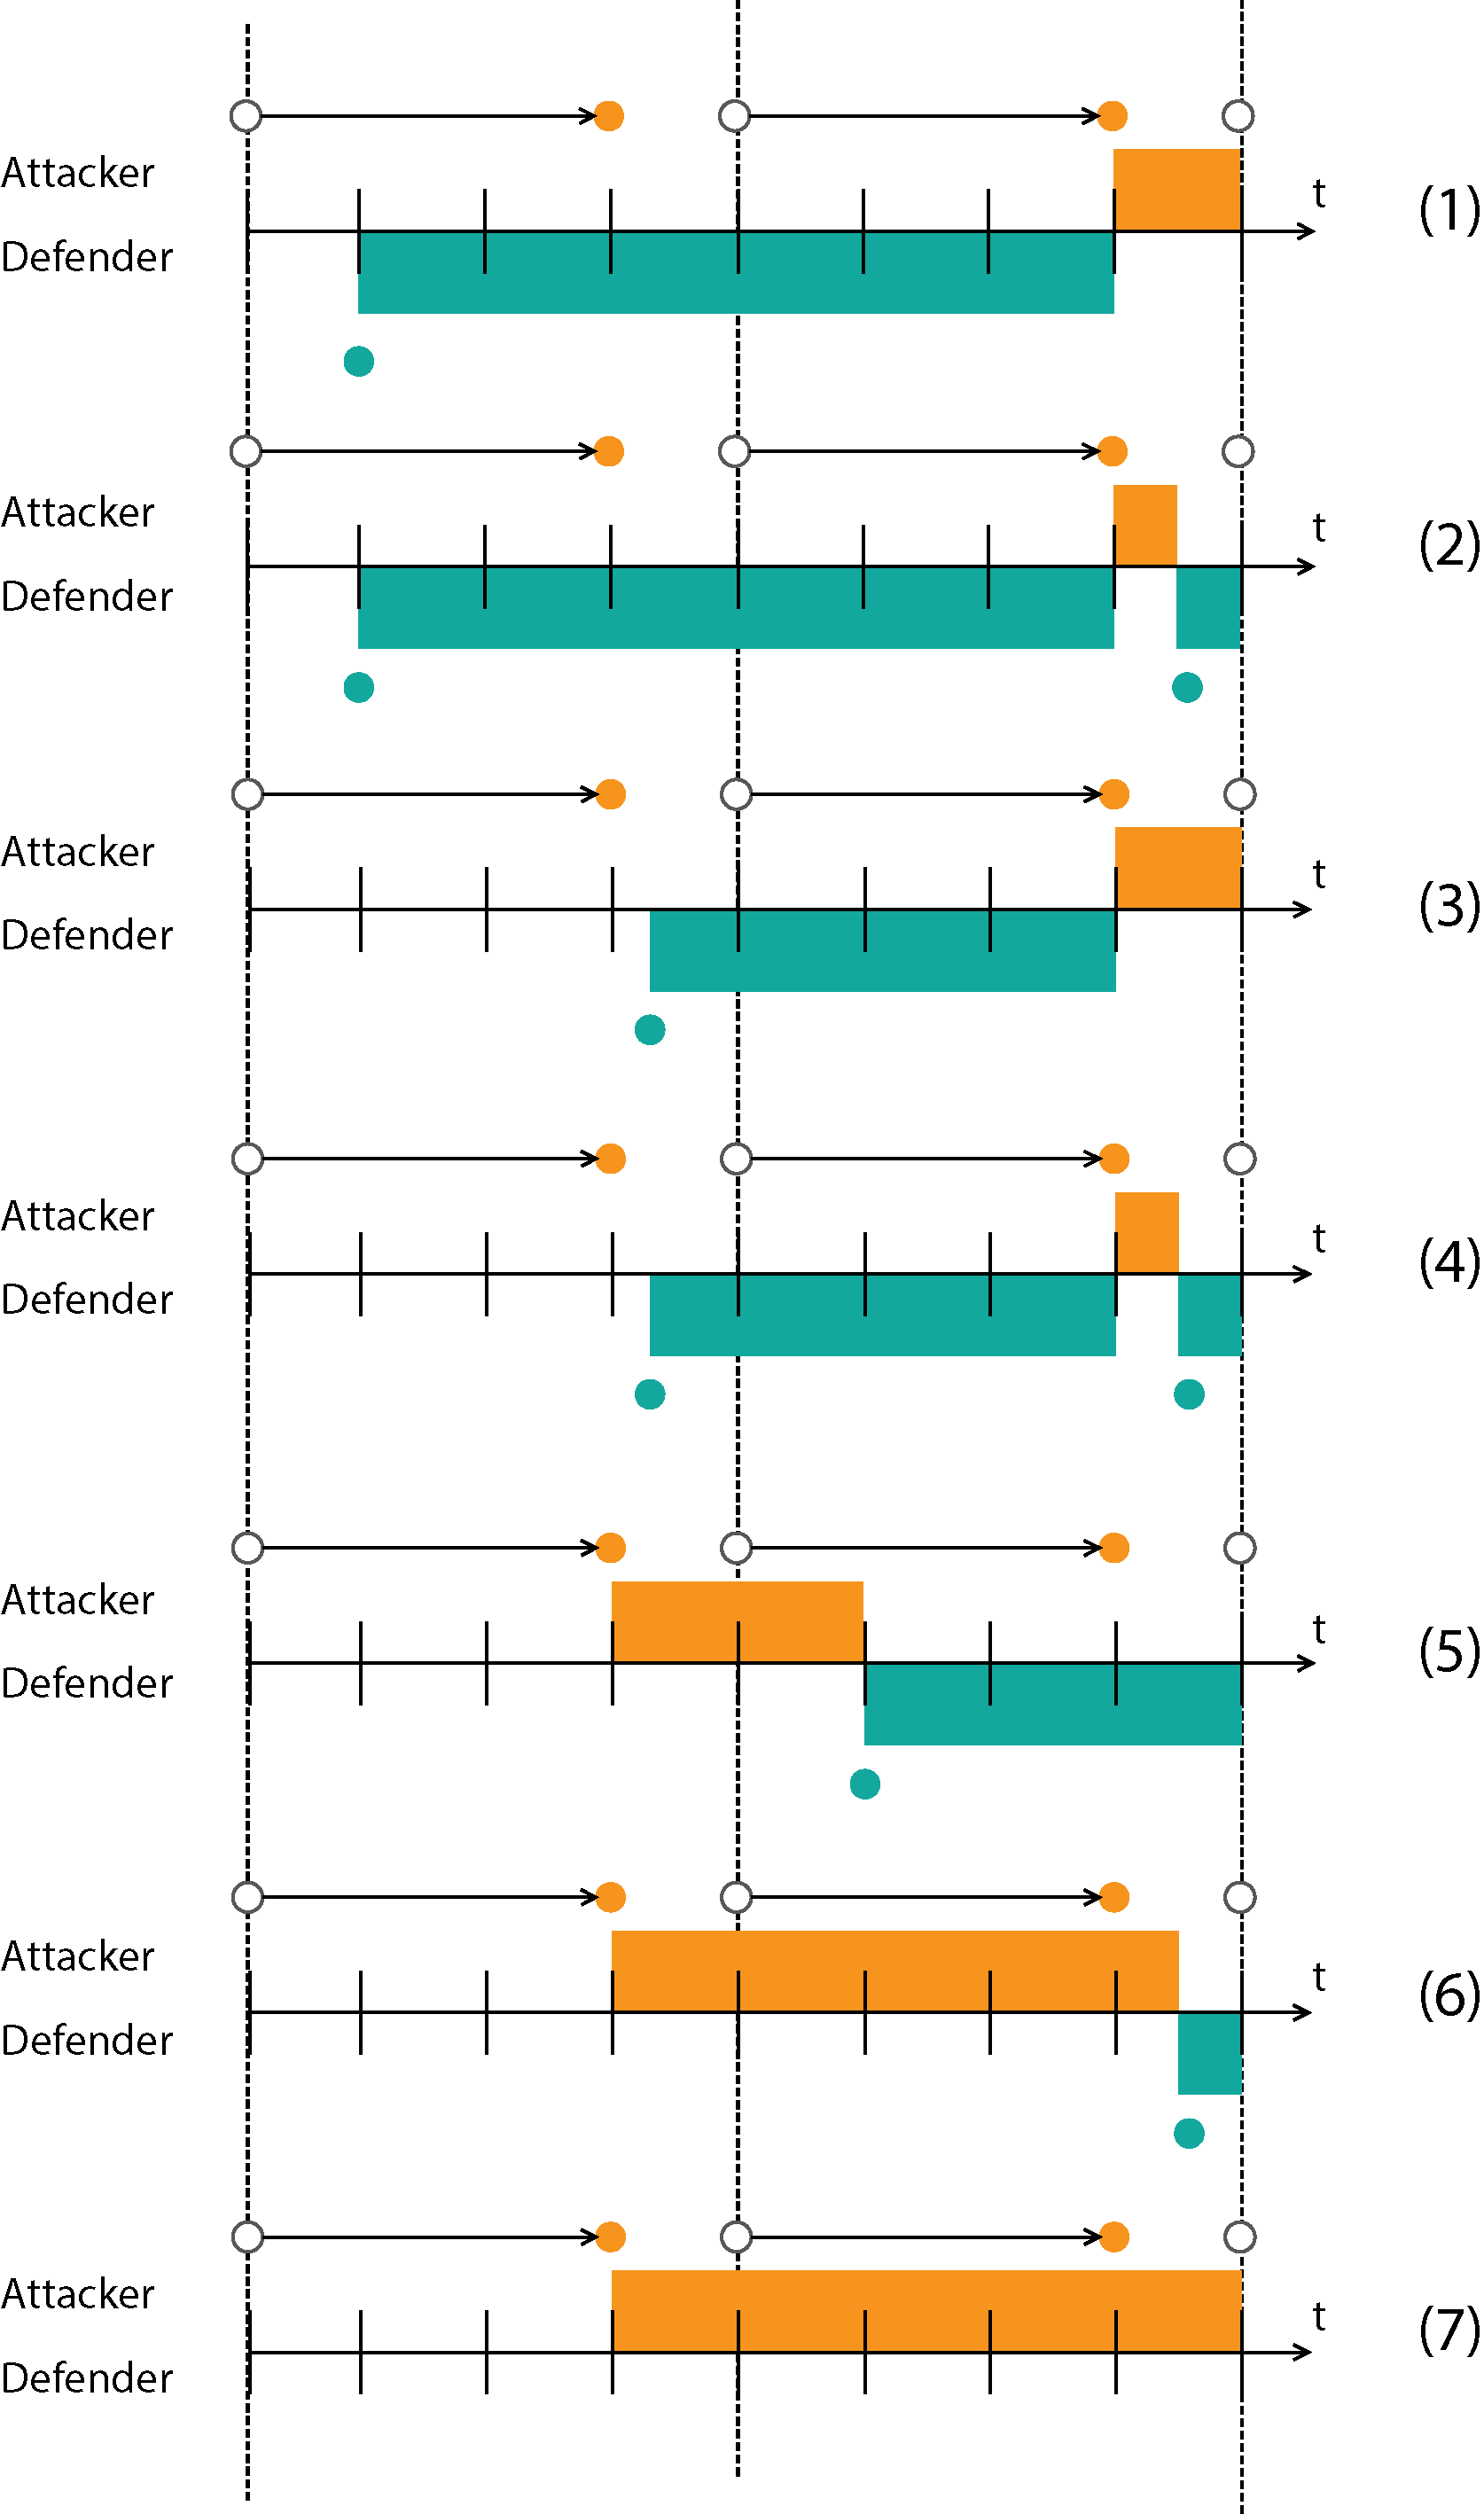
\includegraphics[scale=0.7]{../../doc/template/Images/FlipItCase2a.png}
\label{fig:case2}
\end{figure}


It is crucial that $ \delta_{D}$ is at least as large as $d + \delta_{A}$. If not, this would mean that the defender can move during the delay in the interval following the interval where the defender already moved. This would mean that there can be an overlap between the average gain of $\dfrac{\delta_{A}}{2}$ and the delay. The above benefit formula would then include to much gain for the defender: the potential overlap during the delay would be counted twice. \\


~~ \\
\subsubsection*{\textbf{Case b:} $d + \delta_{A} \geq \delta_{D}$}
~~~\\

To obtain the formula in case of a too long delay, we therefore need to subtract this overlapping gain from the above formula. 
Since $\delta_{D} \geq \delta_{A}$, if the defender enters the interval immediately after the attacker has played, then the defender cannot have played in the previous interval. In that case, there is no overlap. So the problem of the overlap only appears if the defenders enters late enough and thus only the last part of the delay is subject to overlap. The larger the difference between the interval of the defender and the attacker, the smaller the risk of overlap. Concretely, only the last part of length $d - (\delta_{D} - \delta_{A})$ is subject to overlap. Hence, the probability of overlap is $\dfrac{ d - (\delta_{D} - \delta_{A})}{\delta_{D}}$ and the gain will be half of this interval:  $\dfrac{ d - (\delta_{D} - \delta_{A})}{2}$.  The gain rate to be subtracted is therefore:\\

\begin{equation*}
\dfrac{1} {\delta_{A}} \cdot \dfrac{d - (\delta_{D} - \delta_{A})}{\delta_{D}} \cdot \dfrac{d - (\delta_{D} - \delta_{A})}{\delta_{D}}
\end{equation*}

The total gain  rate of the defender is obtained by subtracting this term from the gain rate of case a:
 \begin{equation*}
\gamma_{D}(\alpha_{D},\alpha_{A}) = \dfrac{\delta_{A}}{\delta_{D}} \cdot \dfrac{(d+\dfrac{\delta_{A}}{2})}{\delta_{A}} - \dfrac{(d - (\delta_{D} - \delta_{A}))^{2}}{2 \delta_{D} \delta_{A}}
\end{equation*}
\begin{equation*}
\gamma_{D}(\alpha_{D},\alpha_{A}) = \dfrac{\delta_{A}}{2\delta_{D}} + \dfrac{d}{\delta_{D}} - \dfrac{(d - (\delta_{D} - \delta_{A}))^{2}}{2 \delta_{D} \delta_{A}}
\end{equation*}\\
This yields in the following benefit formula:
\begin{equation*}
\beta_{D}(\alpha_{D},\alpha_{A}) = \dfrac{\delta_{A}}{2\delta_{D}} + \dfrac{d}{\delta_{D}} - k_{D} \alpha_{D} - \dfrac{(d - (\delta_{D} - \delta_{A}))^{2}}{2 \delta_{D} \delta_{A}}
\end{equation*}\\
 
The benefit for the attacker will be as follows:
\begin{equation*}
\beta_{A}(\alpha_{D},\alpha_{A}) = 1 -\dfrac{\delta_{A}}{2\delta_{D}} - \dfrac{d}{\delta_{D}} - k_{A} \alpha_{A} + \dfrac{(d - (\delta_{D} - \delta_{A}))^{2}}{2 \delta_{D} \delta_{A}}
\end{equation*}\\



% ... en zo verder tot
%\chapter{The Final Chapter}
\label{cha:n}


\section{chap}

%%% Local Variables: 
%%% mode: latex
%%% TeX-master: "thesis"
%%% End: 

\chapter{Conclusion}
\label{cha:conclusion}
The final chapter contains the overall conclusion. It also contains
suggestions for future work and industrial applications.

\lipsum[1-7]

%%% Local Variables: 
%%% mode: latex
%%% TeX-master: "thesis"
%%% End: 


% Indien er bijlagen zijn:
%\appendixpage*          % indien gewenst
%\appendix
%\chapter{The First Appendix}
\label{app:A}
Appendices hold useful data which is not essential to understand the work
done in the master thesis. An example is a (program) source.
An appendix can also have sections as well as figures and references.

\section{More Lorem}


%%% Local Variables: 
%%% mode: latex
%%% TeX-master: "thesis"
%%% End: 

% ... en zo verder tot
%\chapter{The Last Appendix}
\label{app:n}
Appendices are numbered with letters, but the sections and subsections use
arabic numerals, as can be seen below.

\section{Lorem 20-24}


%%% Local Variables: 
%%% mode: latex
%%% TeX-master: "thesis"
%%% End: 


\backmatter
% Na de bijlagen plaatst men nog de bibliografie.
% Je kan de  standaard "abbrv" bibliografiestijl vervangen door een andere. plainnat
\bibliographystyle{abbrv}
\bibliography{reffiess}

\end{document}

%%% Local Variables: 
%%% mode: latex
%%% TeX-master: t
%%% End: 

%@Misc{Coursera,
%author = {Coursera},
%title = {Game Theory by Matthew O. Jackson, Kevin Leyton-Brown, Yoav Shoham},
%howpublished = {https://class.coursera.org/gametheory-004}, last checked on 2015-02-22}
%}
%
%
%@Misc{Symantec,
%author = {Symentec},
%title = {2014 Internet Security Threat Report, Volume 19},
%howpublished = {http://www.symantec.com/content/en/us/enterprise/other-resources/b-istr-appendices-v19-221284438.en-us.pdf}, last checked on 2015-02-22}
%}